% 150 câu đã gỡ khỏi ngân hàng (chuyen_dang) — chép lại vào file dạng để khôi phục

% từ: cau-hoi/lop10/0D1_Menh_de_Tap_hop/0D1-1-2_Tinh_dung_sai_cua_menh_de.tex
\begin{ex}%[0D1H1-2]%[ma:2e1e8422]
	Cho hình chữ nhật $ABCD$ có $AB=3$, $BC=4$.  Tính độ dài của vectơ $\overrightarrow{CA}$.
	\choice 
		{\True $\left|\overrightarrow{CA}\right|=5$} 
		{$\left|\overrightarrow{CA}\right|=25$} 
		{$\left|\overrightarrow{CA}\right|=7$} 
		{$\left|\overrightarrow{CA}\right|=\sqrt  7 $}
	\loigiai{ 
	\immini 
		{Xét tam giác $ABC$ vuông tại  $B$, ta có\\ $\left|\overrightarrow{CA}\right|=CA=\sqrt{AB^2+BC^2}=5$.}
		{ 
		\begin{tikzpicture}[scale=1,line join=round,line cap=round,font=\footnotesize,>=stealth]
				\def\d{4} 
				 \def\r{3}
				 \path (0:0) coordinate (B)
					++(0:\d) coordinate  (C)
					++(90:\r) coordinate (D) 
					++(180:\d) coordinate (A); 
				 \draw (A)--(B)--(C)--(D)--cycle (C)--(A);
				 \foreach \x/ \goc in {A/135,B/-135,C/-45,D/45}
				\fill  (\x) circle (1pt)
					 ($(\x)+(\goc:3mm)$) node {$\x$};
			\end{tikzpicture}
		} 
	} 
\end{ex}

% từ: cau-hoi/lop10/0D1_Menh_de_Tap_hop/0D1-1-2_Tinh_dung_sai_cua_menh_de.tex
\begin{bt}%[0D1N1-2]%[ma:86cd4327]
	Cho tứ giác $ABCD$. Gọi $M$, $N$, $P$, $Q$ lần lượt là trung  điểm của $AB$, $BC$, $CD$, $DA$. Từ các điểm đã cho số các vectơ cùng hướng với $\overrightarrow{MN}$ là
	 \shortans{2}
	\loigiai{\begin{center}
		\begin{tikzpicture}[>=stealth,line join=round,line cap=round,font=\footnotesize,scale=0.8]
				 \path
					(1,4) coordinate  (B)
					(0,0) coordinate (A) 
					(6,0) coordinate (D) 
					(4.2,3.5) coordinate  (C)
					($(B)!0.5!(A)$) coordinate (M) 
					($(B)!0.5!(C)$) coordinate (N) 
					 ($(D)!0.5!(C)$) coordinate (P)
					($(D)!0.5!(A)$) coordinate  (Q);
				\draw (A)--(B)--(C)--(D)--(A) 
					(M)--(N) 
					(A)--(C) 
					 (P)--(Q)--cycle;
				\foreach \x/\g in {B/90,A/200,C/30,D/30,M/130,N/90,P/30,Q/-50} \fill (\x) circle (1pt) +(\g:3mm) node[scale=.8]  {$\x$};
			\end{tikzpicture}
	\end{center}
	Ta có  $MN \parallel PQ$, $MN=PQ$ (do cùng song song và bằng $\dfrac{1}{2}AC$). Do đó $MNPQ$ là hình bình hành.\\
	Vậy  các vectơ cùng hướng với $\overrightarrow{MN}$ là $\overrightarrow{QP}$, $\overrightarrow{AC}$.
 }
\end{bt}

% từ: cau-hoi/lop10/0D1_Menh_de_Tap_hop/0D1-1-2_Tinh_dung_sai_cua_menh_de.tex
\begin{ex}%[0D1H1-2]%[ma:34076cc1]
	Cho tứ diện $ ABCD$. Gọi $ M,N$ lần lượt là trung điểm của $ AB$ và $ CD$. Mặt phẳng $ (\alpha)$ qua $ MN$ cắt  $ AD,BC$ lần lượt tại $ P$ và $ Q$. Biết $ MP$ cắt $ NQ$ tại $ I$. Hỏi ba điểm $ I,B,D$ có thẳng hàng chọn $1$, không thẳng hàng chọn $2$, trùng nhau chọn $3$, không nằm ở trường hợp nào của các lựa chọn trước thì chọn $4$.\\
	 \shortans{1}
	 \loigiai{
		\begin{center}
			\tikzset{every picture/.style={line width=0.75pt}} 
			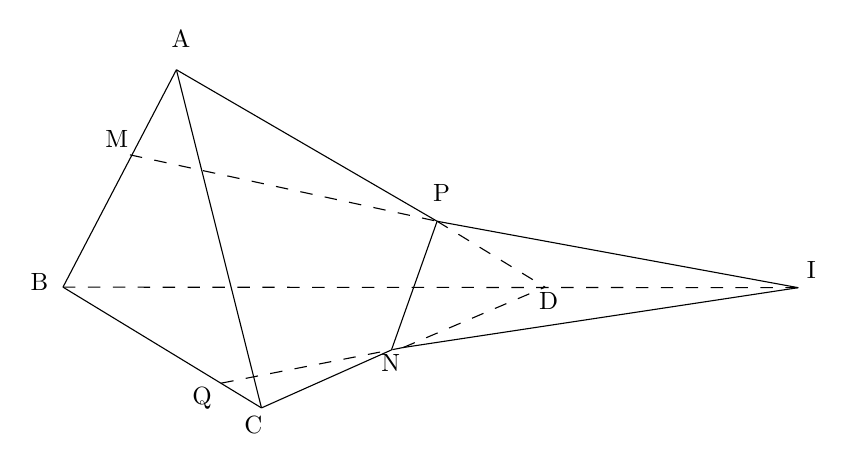
\begin{tikzpicture}[x=0.75pt,y=0.75pt,yscale=-1,xscale=1]
					\draw [dash pattern={on 4.5pt off  4.5pt}] (183.75,137.74) -- (538,138);
					\draw [dash pattern={on  4.5pt off 4.5pt}] (347.69,166.83) -- (416.01,137.74);
					\draw (183.75,137.74) -- (279.38,195.93); 
					\draw (238.39,33) --  (279.38,195.93);
					\draw (238.39,33)  -- (183.75,137.74);
					 \draw (238.39,33) -- (364,106);
					\draw (364,106) -- (342,168); 
					\draw [dash pattern={on 4.5pt off 4.5pt}]  (216,74) -- (364,106);
					\draw  [dash pattern={on 4.5pt off 4.5pt}] (260,184) -- (347.69,166.83);
					\draw (347.69,166.83) -- (538,138); 
					\draw (364,106) -- (538,138); 
					 \draw [dash pattern={on 4.5pt off 4.5pt}] (364,106) -- (416.01,137.74);
					\draw (342,168) -- (279.38,195.93); 
					\draw (541,124) node  [anchor=north west][inner sep=0.75pt] [align=left] {I};
					\draw  (235,13) node [anchor=north west][inner sep=0.75pt] [align=left] {A};
					 \draw (167,130) node [anchor=north west][inner sep=0.75pt] [align=left] {B};
					\draw (203,61) node  [anchor=north west][inner sep=0.75pt] [align=left] {M};
					\draw (361,87) node [anchor=north  west][inner sep=0.75pt] [align=left] {P};
					\draw (412,139) node [anchor=north west][inner sep=0.75pt] [align=left] {D}; 
					\draw (270,199) node [anchor=north west][inner sep=0.75pt] [align=left]  {C};
					\draw (336,169) node [anchor=north west][inner  sep=0.75pt] [align=left] {N};
					\draw (245,185) node [anchor=north west][inner sep=0.75pt]  [align=left] {Q};
				\end{tikzpicture}
		\end{center}
		Ta có:  $ (ABD)\cap (BCD)=BD$.\\
		Mặt  khác: $\heva{
		 {I\in MP,MP\subset (ABD)}\\
		{I\in NQ,NQ\subset  (BCD)}
		 }$\\
		 $\Rightarrow I\in (ABD)\cap (BCD)$.\\
		 Do đó $ I$ thuộc giao tuyến của hai mặt phẳng $ (ABD)$ và $ (BCD)$ hay $ I\in BD$.\\
	Vậy ba điểm $ I,B,D$  thẳng hàng.}
\end{ex}

% từ: cau-hoi/lop10/0D1_Menh_de_Tap_hop/0D1-2-3_Ky_hieu_khoang_doan_nua_khoang.tex
\begin{ex}%[0D1H2-3]%[ma:8406377b]
	Cho $A=[-1;  3]$; $B=(2; 5)$. Tìm mệnh đề \textbf{sai}.
	 \choice
		{$B \setminus  A=(3; 5)$}
		{$A \cap  B=(2; 3]$}
		{$A \setminus  B=[-1; 2]$}
		{\True $A \cup B=[-1; 5]$} 
	\loigiai{ 
		\begin{center}
			
\begin{tikzpicture}[scale=1,>=stealth,font=\footnotesize,line join=round,line cap=round]
					\draw [-stealth]  (0,0)--(6,0);
					 \path (1,0) node{$[$}
						(1,-0.1) node[below]{$-1$} 
						 (-.5,0) node[left]{$[-1; 5)$};
					 \path (3.5,0) node{$)$}
						 (3.5,-0.1) node[below]{$5$};
					\foreach \x in{0,0.1,...,1}  \draw (\x,0)--++(45:.08)
						 (\x,0)--++(-135:.08);
					 \foreach \x in{3.6,3.7,...,5.8} \draw (\x,0)--++(45:.08)
						 (\x,0)--++(-135:.08);
				\end{tikzpicture}
		\end{center}
		Ta có $A \cup B=[-1; 5)$. 
	 }
\end{ex}

% từ: cau-hoi/lop10/0D2_BPT_va_he_BPT_bac_nhat_hai_an/0D2-1-2_Mien_nghiem_cua_BPT_bac_nhat_hai_an.tex
\begin{bt}%[0D2V1-2]%[ma:508ea489]
	Cho tam giác $ABC$ có $A\left(1;2\right)$, $B\left(-3;-1\right)$ và $C\left(3;-4\right)$. Tìm điều kiện của tham số $m$ để điểm  $M\left(m;\dfrac{m-5}{3}\right)$ nằm bên trong tam giác $ABC$.
	\loigiai{ 
		\begin{center}
			\begin{tikzpicture}[scale=.8,>=stealth,font=\footnotesize,line join=round,line cap=round]
					 \path
						(1,2) coordinate (A) 
						 (-3,-1) coordinate (B)
						(3,-4) coordinate (C) 
						(1,-1)  coordinate (M);
					\draw[fill=cyan!50](A)--(B)--(C)--cycle; 
					\draw[->]  (-4,0)--(4,0) node[below]{$x$};
					\draw[->] (0,-5)--(0,3) node[left]{$y$}; 
					\node at  (0,0) [below left]{$O$};
					 \foreach \x/\g in {A/90,B/180,C/-45,M/0}
					\fill[black] (\x) circle (1pt) 
						 ($(\g:3mm)+(\x)$) node {$\x$};
				\end{tikzpicture}
		\end{center}
		Phương trình đường thẳng $AB\colon\dfrac{x-1}{-3-1}=\dfrac{y-2}{-1-2}\Leftrightarrow 3x-4y+5=0$.\\ 
		Phương trình đường thẳng  $BC\colon\dfrac{x+3}{3+3}=\dfrac{y+1}{-4+1}\Leftrightarrow x+2y+5=0$.\\
		Phương trình đường thẳng $AC\colon\dfrac{x-1}{3-1}=\dfrac{y-2}{-4-2}\Leftrightarrow  3x+y-5=0$.\\
		Điều kiện cần và đủ để điểm $M$ nằm bên trong tam giác $ABC$ là điểm $M$ cùng với mỗi đỉnh $A$, $B$, $C$ lần lượt  cùng phía với nhau đối với cạnh $BC$, $CA$, $AB$.
		\begin{itemize}
			 \item $M$ và $A$ nằm cùng phí đối với $BC$ $\Leftrightarrow\left(1+4+5\right)\left(m+2\dfrac{m-5}{3}+5\right)>0\Leftrightarrow m>-1$.
			\item $M$  và $B$ nằm cùng phí đối với $AC$ $\Leftrightarrow \left(-9-1-5\right)\left(3m+\dfrac{m-5}{3}-5\right)>0\Leftrightarrow m<2$.
			\item $M$ và $C$ nằm cùng phí đối với $AB$ $\Leftrightarrow \left(9+16+5\right)\left(3m-4\dfrac{m-5}{3}+5\right)>0\Leftrightarrow m>-7$. 
		\end{itemize}
		Suy ra $-1<m<2$ thỏa mãn điểm $M\left(m;\dfrac{m-5}{3}\right)$ nằm bên  trong tam giác $ABC$.
	 }
\end{bt}

% từ: cau-hoi/lop10/0D3_Ham_so_bac_hai_va_do_thi/0D3-1-1_Xac_dinh_mot_ham_so.tex
\begin{ex}%[0D3Y1-1]%[ma:f7e13597]
	Có $100$ tấm thẻ được đánh số từ  $1$ đến $100$. Lấy ngẫu nhiên $5$ thẻ. Số phần tử của không gian mẫu
	 là
	\choice 
		 {\True $n(\Omega)=\mathrm{C}_{100}^5$}
		{$n(\Omega)=\mathrm{A}_{100}^5$} 
		 {$n(\Omega)=\mathrm{C}_{100}^1$}
		{$n(\Omega)=\mathrm{A}_{100}^1$} 
	\loigiai{ 
		Ta có $n(\Omega)=\mathrm{C}_{100}^5$. 
	} 
\end{ex}

% từ: cau-hoi/lop10/0D3_Ham_so_bac_hai_va_do_thi/0D3-1-3_Gia_tri_cua_ham_so.tex
\begin{bt}%[0D3H1-3]%[ma:5cb5cb78]
	Cho hàm số $f(x)=\heva{&1, &\text{~khi~} \, x=2\\ &\dfrac{1}{x-2}, &\text{~khi~} \, x\ne 2}$.  Giải phương trình $f(x)=\dfrac{x+1}{x-2}$.
	 \loigiai{
		 Xét phương trình $f(x)=\dfrac{x+1}{x-2}$.\\
		Điều kiện $x\ne 2$,  khi đó $f(x)=\dfrac{1}{x-2}$.\\
		Ta có  phương trình $\dfrac{1}{x-2}=\dfrac{x+1}{x-2} \Leftrightarrow x+1=1\Leftrightarrow x=0$.\\
		Vậy tập nghiệm  phương trình $S=\{ 0\}$.
	 }
\end{bt}

% từ: cau-hoi/lop10/0D3_Ham_so_bac_hai_va_do_thi/0D3-1-4_Do_thi_cua_ham_so.tex
\begin{ex}%[0D3H1-4]%[ma:b5e8e007]
	\immini{Cho hàm số $y=f(x)$ có đồ thị như hình vẽ bên. Mỗi kết quả dưới đây đúng hay sai?}{ 
	\begin{tikzpicture}[scale=1,font=\footnotesize,line join=round,line cap=round,>=stealth]
			\draw  [->] (-3,0)--(3,0) node[below]{$x$};
			\draw  [->] (0,-2)--(0,2) node[left]{$y$};
			 \draw[fill=black] (0,0) circle (1pt) node[below left]{$O$};
			\clip (-3,-2) rectangle  (3,2);
			\draw[name path=c1,smooth,samples=300,domain=-3:0] plot (\x,{-1}); 
			\draw[name  path=c2,smooth,samples=300,domain=1:3] plot (\x,{1});
			 \draw (0,-1)--(1,1);
			\foreach \i  in {-2,-1,1,2} \draw [fill=black] (\i,0) circle (1pt) node[below]{$\i$};
			\foreach \j in {1}  \draw [fill=black] (0,\j) circle (1pt) node[left]{$\j$};
			\draw[fill=black] (0,-1) circle  (1pt) node[right]{$-1$};
			\draw[fill=black] (1,1) circle (1pt); 
		\end{tikzpicture}
	} 
	 \choiceTF
		 {$f(1)=0$}
		{\True $f(-2)<f(2)$} 
		{\True Điểm $\left(-2024;-1\right)$ thuộc đồ thị hàm số} 
		 {\True $-1\le f(x)$, $\forall x\in\mathscr{D}$}
	\loigiai{ 
		\begin{itemchoice}
			 \itemch $f(1)=1$.
			\itemch  Do $f(-2)=-1<f(2)=1$.
			\itemch Từ đồ thị của hàm số suy ra điểm $\left(-2024;-1\right)$ thuộc đồ  thị hàm số.
			\itemch Từ đồ thị ta  có $f(x)\ge -1$.
		\end{itemchoice}
	 }
\end{ex}

% từ: cau-hoi/lop10/0D3_Ham_so_bac_hai_va_do_thi/0D3-1-5_Tinh_dong_bien_nghich_bien.tex
\begin{ex}%[0D3N1-5]%[ma:1e820480]
	Cho hàm số $y=f(x)$ có đồ thị  là đường gấp khúc như hình dưới.
	\begin{center}
		\begin{tikzpicture}[scale=0.7,font=\footnotesize,line join=round,line cap=round,>=stealth]
				\def\xmin{-4} 
				\def\xmax{7} 
				 \def\ymin{0}
				 \def\ymax{5}
				\draw[->] (\xmin-1,0)--(\xmax+1,0) node[below] {$x$}; 
				\draw[->]  (0,\ymin-1)--(0,\ymax+1) node[left] {$y$};
				\draw (0,0) node [below left] {$O$}; 
				 \foreach \x in {-4,-3,-2,-1,1,2,3,4,5,6,7} \draw (\x,0.1)--(\x,-0.1) node [below] {$\x$};
				 \foreach \y in {1,5} \draw (0.1,\y)--(-0.1,\y) node [left] {$\y$};
				\clip  (\xmin-0.1,\ymin) rectangle (\xmax+0.1,\ymax);
				\draw  (-4,2)--(-3,0)--(-1,3)--(0,5)--(2,2)--(4,1)--(5,2)--(7,3);
				\draw[dashed]  (-4,0)|-(0,2)
					(-1,0)|-(0,3) 
					 (2,0)|-(0,2)
					(4,0)|-(0,1) 
					(5,0)|-(0,2) 
					 (7,0)|-(0,3);
				 \node[above left] at (0,2) {$2$};
				 \node[above left] at (0,3) {$3$};
			\end{tikzpicture}
	\end{center}
	Khi  đó:
	\choiceTF 
		{Tập giá trị  hàm số $T=[-4;7]$}
		 {\True Ta thấy điểm $(-4;2)$, $(4;1)$ thuộc đồ thị hàm số, điểm $(2;3)$ không thuộc đồ thị hàm số}
		 {\True Ta có $f(-1)=3$, $f(5)=2$}
		{\True Hàm số đã cho đồng biến trên các khoảng $(-3;0)$, $(4;7)$;  hàm số nghịch biến trên các khoảng $(-4;-3)$, $(0;4)$}
	\loigiai{ 
		\begin{itemchoice}
			\itemch Sai. Tập xác  định hàm số là $\mathscr{D}=[-4;7]$.\\
			Tập giá  trị hàm số là $T=[0;5]$.
			\itemch Đúng. Ta thấy điểm $(-4;2)$, $(4;1)$ thuộc đồ thị hàm số, điểm $(2;3)$ không thuộc đồ  thị hàm số.
			 \itemch Đúng. Ta có $f(-1)=3$, $f(5)=2$.
			\itemch Đúng. Hàm số đã cho đồng biến trên các khoảng $(-3;0)$,  $(4;7)$; hàm số nghịch biến trên các khoảng $(-4;-3)$, $(0;4)$.
	\end{itemchoice}}
\end{ex}

% từ: cau-hoi/lop10/0D3_Ham_so_bac_hai_va_do_thi/0D3-1-5_Tinh_dong_bien_nghich_bien.tex
\begin{bt}%[0D3H1-5]%[Dự án đề kiểm tra HKII NH22-23- Nguyễn Ngọc Nguyên]%[THPT Nguyễn Thượng Hiền]%[ma:94b6089c]
	\immini{Cho hàm số xác định trên đoạn $[-3;2]$ như hình bên, hãy xác định các khoảng biến thiên và tập giá trị của hàm số đó trên đoạn $[-3;2]$.}{
	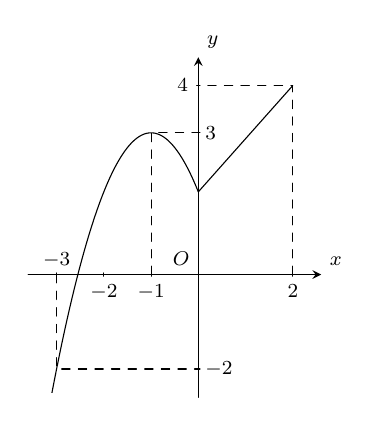
\begin{tikzpicture}[scale=1, font=\footnotesize, line join=round, line cap=round, >=stealth]
		\begin{scope}[scale=.6]
			\draw[->] (-3.6,0)--(2.6,0) node[above right] {$x$};
			\draw[->] (0,-2.6)--(0,4.6) node[above right] {$y$};
			\draw (0,0) node [above left] {$O$};
			\foreach \x in {-2,-1,2}
			\draw[thin] (\x,1pt)--(\x,-1pt) node [below] {$\x$};
			\foreach \x in {-3}
			\draw[thin] (\x,1pt)--(\x,-1pt) node [above] {$\x$};
			\foreach \y in {-2,3}
			\draw[thin] (1pt,\y)--(-1pt,\y) node [right] {$\y$};
			\foreach \y in {4}
			\draw[thin] (1pt,\y)--(-1pt,\y) node [left] {$\y$};
			\draw[dashed,thin](-1,0)--(-1,3)--(0,3);
			\draw[dashed,thin](-3,0)--(-3,-2)--(0,-2);
			\draw (0,7/4)--(2,4);
			\draw[dashed,thin] (2,0)--(2,4)--(0,4);
			\begin{scope}
				\clip (-3.5,-2.5) rectangle (2.5,4.5);
				\draw[samples=200,domain=-3.5:0,smooth,variable=\x] plot (\x,{-5/4*(\x)^2+-5/2*(\x)+7/4});
			\end{scope}
		\end{scope}
	\end{tikzpicture}
}
\loigiai{
Đồ thị hàm số đi lên trong các khoảng $(-3;-1)$ và $(0;2)$ nên hàm số đồng biến trên khoảng $(-3;-1)$ và $(0;2)$.\\
Đồ thị hàm số đi xuống trong khoảng	$(-1{,}0)$ nên hàm số nghịch biến trên khoảng $(-1{,}0)$.\\
Điểm thấp nhất nằm trên đồ thị hàm số trong đoạn $[-3;2]$ có tung độ là $-2$. \\
Điểm cao nhất nằm trên đồ thị hàm số trong đoạn $[-3;2]$ có tung độ là $4$.\\
Do đó tập giá trị của hàm số trên đoạn $[-3;2]$ là $T=[-2;4]$.}
\end{bt}

% từ: cau-hoi/lop10/0D3_Ham_so_bac_hai_va_do_thi/0D3-1-5_Tinh_dong_bien_nghich_bien.tex
\begin{bt}%[0D3H1-5]%[Tex hóa SGK CD-CT,T7/22, Đoàn Minh Tân]%[ma:aea69b5e]
	\immini{Tìm khoảng đồng biến, nghịch biến của hàm số có đồ thị như hình vẽ}
	{
		\begin{tikzpicture}[scale=0.7, font=\footnotesize, line join=round, line cap=round,>=stealth]
			\def \xmin{-2};
			\def \xmax{10};
			\def \ymin{-3};
			\def \ymax{7};
			\draw[->] (\xmin, 0.) -- (\xmax,0.) node[anchor=north] {$x$};
			\draw[->] (0.,\ymin) -- (0.,\ymax) node[anchor=west] {$y$};
			\clip(\xmin-0.1,\ymin-0.1) rectangle (\xmax+0.1,\ymax+0.1);
			\draw[smooth] plot[domain=-1:1] (\x,{-0.5*(\x)^2+1.5*(\x)+3});
			\draw[smooth] plot[domain=1:5] (\x,{-(\x)^2/6-0.5*(\x)+14/3});
			\draw[smooth] plot[domain=5:9] (\x,{2*(\x)-12});
			\foreach \i in {-1,1,2,3,4,5,6,7,8,9}
			\draw[fill=black] (\i,0) circle(1pt) node[below]{$\i$};
			\foreach \j in {-1,-2,1,2,3,4,5,6}
			\draw[fill=black] (0,\j) circle(1pt) node[left]{$\j$};
			\draw[fill=black] (0,0) circle(1pt) node[below left]{$O$} (1,4) circle(1pt) (5,-2) circle(1pt) (9,6) circle(1pt) (-1,1) circle(1pt);
			\draw[dashed] (-1,0)|-(0,1) (5,0)|-(0,-2) (9,0)|-(0,6) (1,0)--(0,4);
		\end{tikzpicture}
	}
	\loigiai{
		Dựa vào đồ thị, suy ra
		\begin{itemize}
			\item Hàm số đồng biến trên các khoảng $(-1;1)$, $(5;9)$.
			\item Hàm số nghịch biến trên khoảng $(1;5)$.
		\end{itemize}	
	}
\end{bt}

% từ: cau-hoi/lop10/0D3_Ham_so_bac_hai_va_do_thi/0D3-2-1_Xac_dinh_ham_so_bac_hai.tex
\begin{ex}%[0D3Y2-1]%[ma:ecac42af]
	Gieo một con xúc sắc cân đối, đồng chất một lần. Xác suất  để xuất hiện mặt chẵn?
	 \choice
		 {\True $\dfrac{1}{2}$}
		{$\dfrac{1}{4}$} 
		 {$\dfrac{1}{6}$}
		{$\dfrac{1}{3}$} 
	 \loigiai{
		Gieo một con xúc sắc cân đối, đồng  chất một lần.\\
		$\Rightarrow$ Số  phần tử của không gian mẫu $n(\Omega)=6$.\\
		Gọi $\mathrm{A}$ là biến cố: \lq\lq Xuất hiện mặt  chẵn\rq\rq $\Rightarrow n(A)=3$.\\
		Vậy xác suất  của biến cố $A$ là $P(A)=\dfrac{3}{6}=\dfrac{1}{2}$.
	} 
\end{ex}

% từ: cau-hoi/lop10/0D3_Ham_so_bac_hai_va_do_thi/0D3-2-2_Bang_bien_thien_tinh_don_dieu_max_min.tex
\begin{bt}%[0D3H2-2]%[Nguyễn Đức Tuệ]%[ma:37a76226]
	Hãy	tìm giá trị lớn nhất $M$ và giá trị nhỏ nhất $m$ trên đoạn $\left[ -2;1 \right]$	của hàm số $y=f(x)=x^2-4x+3$. 
	\loigiai{Hàm số $y=x^2-4x+3$ có $a=1>0$ nên bề lõm hướng lên.\\
		Hoành độ đỉnh $x=-\dfrac{b}{2a}=2\notin \left[ -2;1 \right]$.\\
		Ta có $\heva{& f\left(-2\right)=15 \\& f\left(1\right)=0}\Rightarrow m=\min \limits_{\left[ -2;1 \right]} y=f\left(1\right)=0; M=\max \limits_{\left[ -2;1 \right]} y=f\left(-2\right)=15$. 
	}
\end{bt}

% từ: cau-hoi/lop10/0D3_Ham_so_bac_hai_va_do_thi/0D3-2-2_Bang_bien_thien_tinh_don_dieu_max_min.tex
\begin{bt}%[0D3H2-2]%[Dự án đề kiểm tra HKI NH22-23 - Nguyễn Ngọc Dũng]%[THPT Hùng Vương]%[ma:8009df40]
Cho hàm số $y=f(x)=-x^2+2x+3$.
\begin{enumerate}
\item Lập bảng biến thiên của hàm số.
\item Dựa vào bảng biến thiên, tìm khoảng đồng biến và khoảng nghịch biến của hàm số.
\end{enumerate}
\dapso{\textbf{a)}  
\begin{tikzpicture}
\tkzTabInit[nocadre,lgt=1.2,espcl=2.5,deltacl=0.6]
{$x$/0.6,$y$/2}{$-\infty$,$1$,$+\infty$}
\tkzTabVar{-/$-\infty$,+/$4$,-/$-\infty$}
\end{tikzpicture}; \textbf{b)} Hàm số đồng biến trên $(-\infty;1)$ và nghịch biến trên $(1;+\infty)$.}
\loigiai{
\begin{enumerate}
\item \begin{itemize}
\item Đỉnh $S$ có tọa độ: $x_S=\dfrac{-b}{2a}=\dfrac{-2}{2\cdot (-1)} = 1$; $y_S=-1^2+2\cdot 1 +3 = 4$.\\
Hay $S(1;4).$
\item Vì hàm số bậc hai có $a=-1<0$ nên có bảng biến thiên như sau:
\begin{center}

\begin{tikzpicture}
\tkzTabInit[nocadre,lgt=1.2,espcl=2.5,deltacl=0.6]
{$x$/0.6,$y$/2}{$-\infty$,$1$,$+\infty$}
\tkzTabVar{-/$-\infty$,+/$4$,-/$-\infty$}
\end{tikzpicture}
\end{center}
\end{itemize}
\item Hàm số đồng biến trên $(-\infty;1)$ và nghịch biến trên $(1;+\infty)$.
\end{enumerate}
}
\end{bt}

% từ: cau-hoi/lop10/0D7_Bat_phuong_trinh_bac_2_mot_an/0D7-1-3_Bai_toan_xet_dau_biet_BXD_do_thi.tex
\begin{bt}%[0D7H1-3]%[Dự án đề kiểm tra HKII NH22-23- Phạm Văn Long]%[THPT Phú Hoà]%[ma:ba3b7d51]
	\begin{enumerate}
		\item Cho hàm số $y=f(x)$ có đồ thị như hình vẽ. Lập bảng xét dấu của $f(x)$.
		\begin{center}
			\begin{tikzpicture}[scale=0.6, font=\footnotesize,line join=round, line cap=round, >=stealth];
				\draw[->] (-4,0) -- (2.5,0) node[below] {\scriptsize $x$};
				\draw[->] (0,-2) -- (0,5) node[left] {\scriptsize $y$};
				\draw (0.1,0.1)node[below left]{\scriptsize $O$};
				\draw[thin,samples=150,smooth,domain=-3.3:1.3] plot(\x,{-1*((\x)^2)-2*(\x)+3});						
				\draw[fill=black]  (-3,0) circle (1.2pt) (1,0) circle (1.2pt);
				\draw (-3.5,0)node[above]{$-3$} (1.3,0)node[above]{$1$};	
			\end{tikzpicture}
		\end{center}
		\item Giải bất phương trình $x^2-8 x+16 \leq 0$.
	\end{enumerate}
\loigiai{
\begin{enumerate}
	\item Bảng xét dấu của $f(x)$.
			\begin{center}
			
\begin{tikzpicture}
				\tkzTabInit[lgt=1.2,espcl=2.5,deltacl=0.6]
				{$x$ /0.6,$y$ /0.6}
				{$-\infty$,$-3$,$1$,$+\infty$}
				\tkzTabLine{,-,$0$,+,$0$,-,}				
			\end{tikzpicture}
		\end{center}
	Từ bảng xét dấu của $f(x)$ ta có
	\begin{itemize}
		\item $f(x)> 0$ khi $x\in \left(-3;1\right)$.
		\item $f(x)<0$ khi $x\in (-\infty;-3)\cup (1;+\infty)$.
		\item $f(x)= 0$ khi $x=-3$ hoặc $x=1$.
	\end{itemize}
	\item Ta có $x^2-8 x+16=0\Leftrightarrow x=4$.\\
	Bảng xét dấu của $f(x)=x^2-8 x+16$.
	\begin{center}
		
\begin{tikzpicture}
			\tkzTabInit[lgt=1.2,espcl=2.5,deltacl=0.6]
			{$x$ /0.6,$y$ /0.6}
			{$-\infty$,$4$,$+\infty$}
			\tkzTabLine{,+,$0$,+,}				
		\end{tikzpicture}
	\end{center}
	Từ bảng xét dấu của $f(x)$ suy ra $x^2-8 x+16 \geq 0\, \forall  \in \mathbb{R}$.\\
	Khi đó suy ra $x^2-8 x+16 \leq 0$ khi $x=4$.\\
	Vậy $S=\{4\}$.
\end{enumerate}
}
\end{bt}

% từ: cau-hoi/lop10/0D7_Bat_phuong_trinh_bac_2_mot_an/0D7-2-1_Bat_phuong_trinh_bac_2_va_ung_dung.tex
\begin{ex}%[0D7H2-1]%[ma:5ed144e6]
	 Tập xác định của hàm số $y=\sqrt{6-x-x^2}$ là
	 \choice
		{\True $\mathscr{D}=[-3;2]$} 
		 {$\mathscr{D}=(-\infty;-3]\cup[2;+\infty)$}
		{$\mathscr{D}=(-\infty;-3)\cup(2;+\infty)$} 
		 {$\mathscr{D}=[-2;3]$}
	\loigiai{ 
		Điều  kiện $6-x-x^2\ge 0$.\\
		 Bảng xét dấu
		\begin{center}
			
\begin{tikzpicture}
					 \tkzTabInit[lgt=2,espcl=2.5,deltacl=0.6]
						{$x$/0.8,$6-x-x^2$/0.8}{$-\infty$,$-3$,$2$,$+\infty$} 
					 \tkzTabLine{,-,0,+,0,-,}
				\end{tikzpicture}
		\end{center}
		Vậy tập xác định của hàm số $y=\sqrt{6-x-x^2}$ là $\mathscr{D}=[-3;2]$. 
	 }
\end{ex}

% từ: cau-hoi/lop10/0D7_Bat_phuong_trinh_bac_2_mot_an/0D7-2-2_Giai_bat_phuong_trinh_bac_hai_biet_BXD_do_thi.tex
\begin{ex}%[0D7N2-2]%[ma:299937c7]
	Cho đồ thị của hàm số bậc hai $f(x)$ như  hình vẽ
	\begin{center}
		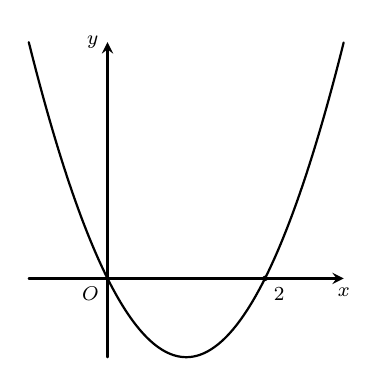
\begin{tikzpicture}[scale=1,font=\footnotesize,line join=round,line cap=round,>=stealth]
				 \draw[thick,->] (-1,0)--(3,0) node[below] {$x$};
				\draw[thick,->] (0,-1)--(0,3) node[left]  {$y$};
				\draw (0,0)  node[below left] {$O$};
				\draw[thick,smooth,samples=200] plot[domain=-1:3] (\x,{(\x)^2-2*(\x)}); 
				\fill  (2,0) circle (1pt) node[below right] {$2$};
			\end{tikzpicture}
	\end{center}
	Tập nghiệm của bất phương trình  $f(x)>0$ là
	 \choice
		{\True $S=(-\infty; 0) \cup  (2;+\infty)$}
		{$S=(0;  2)$}
		{$S=(-\infty; 0]  \cup [2;+\infty)$}
		{$S=(2;+\infty)$} 
	\loigiai{ 
		Dựa vào đồ thị hàm số bậc hai $f(x)$ đã cho, ta thấy phần đồ  thị nằm phía trên trục hoành khi $x<0$ hoặc $x>2$.\\
		Vậy tập nghiệm của bất phương trình $f(x)>0$ là $S=(-\infty; 0) \cup  (2;+\infty)$.
	} 
\end{ex}

% từ: cau-hoi/lop10/0D7_Bat_phuong_trinh_bac_2_mot_an/0D7-2-2_Giai_bat_phuong_trinh_bac_hai_biet_BXD_do_thi.tex
\begin{ex}%[0D7H2-2]%[ma:db0d1e61]
	Cho tam thức bậc hai $f(x)=-x^2-4x+5$. Tìm tất cả  giá trị của $x$ để $f(x)\ge 0$.
	 \choice
		{$x\in \left(-\infty;-1\right]\cup \left[5;+\infty \right)$} 
		{$x\in \left[-1; 5\right]$} 
		{\True  $x\in \left[-5; 1\right]$}
		{$x\in \left(-5; 1\right)$} 
	 \loigiai{
		Xét tam  thức $f(x)=-x^2-4x+5$. Ta có
		\begin{itemize}
			\item $a=-1<  0$;
			\item $\Delta=36> 0$ nên tam thức $f(x)$ có hai nghiệm $x=1$ và $x=-5$. 
		\end{itemize}
		Bảng xét dấu 
		\begin{center}
			
\begin{tikzpicture}[>=stealth]
					\tkzTabInit[nocadre=false,lgt=1.5,espcl=2,deltacl=0.6]{$x$/.7,$f  (x)$/.7}
						{$-\infty$,$-5$,$1$,$+\infty$} 
					\tkzTabLine{,-,$0$,+,$0$,-,} 
				\end{tikzpicture}
		\end{center}
		Suy ra $f(x)\ge 0$ khi $-5\le x\le  1$.
	 }
\end{ex}

% từ: cau-hoi/lop10/0D7_Bat_phuong_trinh_bac_2_mot_an/0D7-2-2_Giai_bat_phuong_trinh_bac_hai_biet_BXD_do_thi.tex
\begin{ex}%[0D7H2-2]%[ma:1d443a21]
	Bảng xét dấu  nào sau đây là bảng xét dấu của tam thức $f(x)=-x^2-x+6$?
	 \choice
		{
\begin{tikzpicture}
		\tkzTabInit[nocadre=false,lgt=1.5,espcl=1.5] 
			{$x$ /0.6,$f  (x)$ /0.6}
			{$-\infty$,$-2$,$3$,$+\infty$} 
		\tkzTabLine{,-,0,+,0,-} 
	\end{tikzpicture}
		 }
		{
\begin{tikzpicture}
		\tkzTabInit[nocadre=false,lgt=1.5,espcl=1.5] 
			 {$x$ /0.6,$f (x)$ /0.6}
			{$-\infty$,$-2$,$3$,$+\infty$} 
		 \tkzTabLine{,+,0,-,0,+}
	\end{tikzpicture}
		} 
		{\True 
\begin{tikzpicture}
		\tkzTabInit[nocadre=false,lgt=1.5,espcl=1.5] 
			 {$x$ /0.6,$f (x)$ /0.6}
			{$-\infty$,$-3$,$2$,$+\infty$} 
		\tkzTabLine{,-,0,+,0,-} 
	\end{tikzpicture}
		 }
		{
\begin{tikzpicture}
		 \tkzTabInit[nocadre=false,lgt=1.5,espcl=1.5]
			{$x$  /0.6,$f (x)$ /0.6}
			{$-\infty$,$-3$,$2$,$+\infty$} 
		 \tkzTabLine{,+,0,-,0,+}
	\end{tikzpicture}
		 }
	\loigiai{ 
		Tam thức $f(x)=-x^2-x+6$ có $\Delta =25>0$, hai nghiệm $x_1=-3$, $x_2=2$  và hệ số $a=-1<0$.\\
		Suy ra bảng xét dấu của $f(x)$  như sau
		\begin{center}
			
\begin{tikzpicture}
					 \tkzTabInit[nocadre=false,lgt=1.5,espcl=1.5]
						{$x$ /0.6,$f (x)$ /0.6} 
						{$-\infty$,$-3$,$2$,$+\infty$} 
					 \tkzTabLine{,-,0,+,0,-}
				\end{tikzpicture}
		\end{center}
	} 
\end{ex}

% từ: cau-hoi/lop10/0D7_Bat_phuong_trinh_bac_2_mot_an/0D7-2-2_Giai_bat_phuong_trinh_bac_hai_biet_BXD_do_thi.tex
\begin{bt}%[0D7H2-2]%[Dự án đề kiểm tra Giữa HKII NH22-23- Thành Lê]%[THPT Nguyễn Công Trứ]%[ma:0dbfddbe]
	Dựa vào đồ thị của hàm số bậc hai tương ứng, hãy xác định tập nghiệm của các bất phương trình bậc hai sau đây
	\begin{enumEX}{2}
		\item $x^2 + 2{,}5x - 1{,}5\geq0$.
		\begin{center}
			\begin{tikzpicture}[line join = round, line cap = round,>=stealth,font=\footnotesize,scale=.8,transform shape]
				\clip (-5,-4.2) rectangle (4.5,5.1);
				\draw[->,line width = 1pt,red] (-4.5,0)--(0,0) node[above  left]{$O$}--(4,0) node[below]{$x$};
				\draw[->,line width = 1pt,red] (0,-4)--(0,5) node[right]{$y$};
				\draw (0,-1.5) node[right] {$\dfrac{-1}{2}$};
				\draw (0,-1.5) circle (2pt);
				%%============
				\foreach \x in {-4,-3,-2,-1,1,2,3} \draw[thin] (\x,2pt)--(\x,-2pt) node [below left,blue] {$\x$};
				\foreach \y in {-4,-3,-2,-1,1,2,3,4} \draw[thin] (2pt,\y)--(-2pt,\y) node [left,blue] {$\y$};
				%%===========
				\draw[samples=100,domain=-4:1.5,smooth] plot (\x, {(\x)^2+5/2*(\x)-3/2});
			\end{tikzpicture}
		\end{center}
		\item $ - x^2 - 8x - 16<0$.
		\begin{center}
			\begin{tikzpicture}[line join = round, line cap = round,>=stealth,font=\footnotesize,scale=.8,transform shape]
			\draw[->,line width = 1pt,red] (-7.5,0)--(0,0) node[below right]{$O$}--(2,0) node[above]{$x$};
			\draw[->,line width = 1pt,red] (0,-7.5)--(0,2) node[right]{$y$};
			%%===============
			\foreach \x in {-7,-6,-5,-4,-3,-2,-1,1} \draw[thin] (\x,2pt)node [above,blue] {$\x$}--(\x,-2pt);
			\foreach \y in {-7,-6,-5,-4,-3,-2,-1,1} \draw[thin] (2pt,\y)--(-2pt,\y) node [left,blue] {$\y$};
			%%==============
			\draw[samples=100,domain=-6.65:-1.35,smooth] plot (\x, {-(\x)^2-8*(\x)-16});
			\end{tikzpicture}
		\end{center}
	\end{enumEX}
	\loigiai{
	\begin{enumEX}{1}
		\item Dựa vào đồ thị, ta có tập nghiệm $\left(-\infty;-3\right]\cup\left[\dfrac{1}{2};+\infty\right)$.
		\item Dựa vào đồ thị, ta có tập nghiệm là $\mathbb{R}\setminus\{-4\}$.
	\end{enumEX}
	}
\end{bt}

% từ: cau-hoi/lop10/0D7_Bat_phuong_trinh_bac_2_mot_an/0D7-2-5_Bat_phuong_trinh_chua_can.tex
\begin{bt}%[0D7H2-5]%[ma:8426019f]
	Số nghiệm  của phương trình sau $\sqrt{2x^2+5x+3}=-3-x$ là
	\shortans{0} 
	\loigiai{ 
		Bình  phương hai vế phương trình đã cho, ta được
		\begin{eqnarray*}
			 &&2x^2+5x+3=(-3-x)^2\\
			&\Rightarrow&  2x^2+5x+3=9+6x+x^2\\
			&\Rightarrow& x^2-x-6=0\\ 
			 &\Rightarrow& \hoac{&x=3\\&x=-2.}
		\end{eqnarray*}
		Thay lần lượt các giá trị trên vào phương trình đã cho ta thấy không có giá trị nào  thỏa mãn.\\
		Vậy phương trình  đã cho vô nghiệm.
	 }
\end{bt}

% từ: cau-hoi/lop10/0D7_Bat_phuong_trinh_bac_2_mot_an/0D7-2-6_Bai_toan_co_tham_so.tex
\begin{bt}%[Bài Giảng K10-K11, Đỗ Viết Lân]%[0D7V2-6]%[ma:16f164c9]
	Tìm các giá trị của tham số $m$ để tam thức bậc hai $3x^2+2(m-1)x+m+4>0,\,\forall x \in \mathbb{R}$.
	\loigiai{
		\allowdisplaybreaks
		\begin{eqnarray*}
			3x^2+2(m-1)x+m+4>0,\,\forall x \in \mathbb{R}&\Leftrightarrow& \heva{& 3>0\\& \left[2(m-1)\right]^2-4\cdot 3\cdot (m+4)<0}\\
			&\Leftrightarrow&4m^2-16m-44<0\\
			&\Leftrightarrow &2-\sqrt{15}<m<2+\sqrt{15}.
		\end{eqnarray*}
	}
\end{bt}

% từ: cau-hoi/lop10/0D7_Bat_phuong_trinh_bac_2_mot_an/0D7-2-6_Bai_toan_co_tham_so.tex
\begin{bt}%[0D7H2-6]%[Tex hóa SGK CD-CT,T7/22, Bùi Mạnh Tiến]%[ma:7771eb38]
	Tìm các giá trị của tham số $m$ để:\\
	\begin{enumerate}
		\item $f(x)=(m+1)x^2+5x+2$ là tam thức bậc hai không đổi dấu trên $\mathbb{R}$;
		\item $f(x)=mx^2-7x+4$ là tam thức bậc hai âm với mọi $x \in \mathbb{R}$;
		\item $f(x)=3x^2-4x+(3m-1)$ là tam thức bậc hai dương với mọi $x \in \mathbb{R}$;
		\item $f(x)=(m^2+1)x^2-3mx+1$ là tam thức bậc hai âm với mọi $x \in \mathbb{R}$.
	\end{enumerate}
	\loigiai{
		\begin{enumerate}
			\item $f(x)$ là tam thức bậc hai không đổi dấu trên $\mathbb{R}$ khi và chỉ khi $m+1 \ne 0$ và $\Delta =25-8(m+1)<0$. Vậy $m>\dfrac{17}{8}$.
			\item $f(x)$ là tam thức bậc hai âm với mọi $x \in \mathbb{R}$ khi và chỉ khi $m<0$ và $\Delta =7^2-16m<0$, nghĩa là $m<0$ và $m>\dfrac{49}{16}$, vô lí.\\
			Vậy không có giá trị nào của tham số $m$ thoả mãn yêu cầu.
			\item Vì $3>0$ nên $f(x)$ là tam thức bậc hai dương với mọi $x \in \mathbb{R}$ khi và chỉ khi $\Delta'=4-3(3m-1)<0$, nghĩa là $m>\dfrac{7}{9}$.
			\item Vì $m^2+1>0$ nên $f(x)$ không thể âm với mọi $x \in \mathbb{R}$.\\
			Vậy không có giá trị nào của tham số $m$ thoả mãn yêu cầu.
		\end{enumerate}
	}
\end{bt}

% từ: cau-hoi/lop10/0D7_Bat_phuong_trinh_bac_2_mot_an/0D7-3-5_Phuong_trinh_khac_quy_ve_phuong_trinh_bac_2.tex
\begin{ex}%[0D7H3-5]%[ma:bc1b104b]
	Nghiệm của phương  trình $-2x^{2}+4x-2=0$ là
	\choice 
		 {$x=-1$}
		{$x=-2$} 
		 {$x=2$}
		{\True $x=1$} 
	\loigiai{ 
		Ta có $-2x^{2}+4x-2=0\Leftrightarrow-2(x-1)^{2}=0\Leftrightarrow x=1$. 
	 }
\end{ex}

% từ: cau-hoi/lop10/0D7_Bat_phuong_trinh_bac_2_mot_an/0D7-3-6_Toan_hinh_toan_thuc_te_ung_dung_phuong_trinh.tex
\begin{ex}%[0D7C3-6]%[ma:bd482827]
	Tam giác $ABC$ vuông tại $A$, có cạnh $AC$ ngắn hơn cạnh $BC$ là $9$ cm. Biết chu vi của tam giác bằng $70$ cm, độ dài  đoạn $AC$ là
	 \choice
		{$21$  cm}
		{\True $20$  cm}
		{$29$  cm}
		{$28$ cm} 
	\loigiai{ 
	\immini{Gọi  độ dài cạnh $AC$ là $x$ cm.\\
		Cạnh $AC$ ngắn hơn cạnh $BC$ là $9$ cm nên độ dài cạnh $BC$ là  $(x+9)$ cm.\\
		Ta có  $AC^2+AB^2=BC^2$ hay
		 \[
		 AB=\sqrt{BC^2-AC^2}=\sqrt{(x+9)^2-x^2}=\sqrt{18x+81}.
		\] 
		Chu vi tam giác  $ABC$ bằng $70$ cm nên
		 \allowdisplaybreaks
		\begin{eqnarray*}
			AB+BC+CA=70 &\Rightarrow&\sqrt{18x+81}+(x+9)+x=70  \\
			&\Rightarrow&\sqrt{18x+81}=61-2x\\ 
			&\Rightarrow&  18x+81=61^2-2\cdot 61 \cdot 2x+4x^2\\
			&\Rightarrow& 4x^2-262x+3640=0\\ 
			 &\Rightarrow&\hoac{&x=20\\ &x=\dfrac{91}{2}.}
		\end{eqnarray*}
		Thay lần lượt các giá trị trên vào phương trình đã cho,  ta thấy $x=20$ thỏa mãn.\\
		Vậy $AC=20$  cm.
		}{\begin{tikzpicture}[scale=0.7,font=\footnotesize,line join=round,line cap=round,>=stealth]
		\coordinate [label=below left:$A$] (A) at  (0,0);
		\coordinate [label=above:$C$](C)  at (0,3);
		\coordinate [label=below: $B$] (B) at (2,0); 
		\draw  (A)--(C)--(B)--(A);
		\foreach \diem in {A,B,C}  \fill (\diem) circle (1.5pt);
		\draw pic[draw,angle radius=2mm]  {right angle = C--A--B};
	\end{tikzpicture}
		 }
	 }
\end{ex}

% từ: cau-hoi/lop10/0D7_Bat_phuong_trinh_bac_2_mot_an/0D7-3-6_Toan_hinh_toan_thuc_te_ung_dung_phuong_trinh.tex
\begin{bt}%[Dự án Bài Giảng 10-11 Nhóm Toán & LaTex, Nguyễn Anh Tuấn]%[0D7V3-6]%[ma:778e346a]
	\immini{
		Một con tàu biển $M$ rời cảng $O$ và chuyển động thẳng theo phương tạo với bờ biển một góc $60^{\circ}$. Trên bờ biển có hai đài quan sát $A$ và $B$ nằm về hai phía so với cảng $O$ và lần lượt cách cảng $O$ khoảng cách $1$ km và $2$ km.
	}{
		\begin{tikzpicture}[line cap=round, line join=round, font=\footnotesize, >=stealth, scale=0.8]
			\tikzset{label style/.style={font=\footnotesize}}
			\path (0,0) coordinate (O)
			(-2,0) coordinate (A)
			(4,0) coordinate (B)
			(60:3.5) coordinate (M);
			\draw (M)--(A)--(O) node[above,pos=0.6]{$1$ km}--(B) node[above, midway]{$2$ km}--(M)--(O) node[midway, right]{$x$ km};
			\foreach\x/\y in {A/-135,O/-90,M/90,B/-45} \draw[fill=black] (\x) circle (2pt)+(\y:0.5) node{$\x$};
			\draw pic[draw,angle radius=8mm]{angle=B--O--M}
			(25:0.6) node{$60^\circ$};
		\end{tikzpicture}	
		
	}
	\begin{enumerate}
		\item Đặt độ dài của $M O$ là $x \mathrm{~km}$. Biểu diễn khoảng cách từ tàu đến $A$ và từ tàu đến $B$ theo $x$.
		\item Tìm $x$ để khoảng cách từ tàu đến $B$ bằng $\dfrac{4}{5}$ khoảng cách từ tàu đến $A$.
		\item Tìm $x$ để khoảng cách từ tàu đến $B$ nhỏ hơn khoảng cách từ tàu đến $O$ đúng $500 \mathrm{~m}$.
	\end{enumerate}
	\textit{Lưu ý: Làm tròn kết quả đến hàng phần trăm.}
	\loigiai{
		\begin{enumerate}
			\item Áp dụng định lí cô-sin, ta có
			\begin{align*}
				MA&=\sqrt{OM^2+OA^2-2OM\cdot OA\cdot \cos 120^\circ}=\sqrt{x^2+x+1},\\
				MB&=\sqrt{OM^2+OB^2-2OM\cdot OB\cdot \cos 60^\circ}=\sqrt{x^2-2x+4}.
			\end{align*}
			\item Theo yêu cầu, ta cần có $MB=\dfrac{4}{5}MA$, suy ra
			\begin{align*}
				&5\sqrt{x^2-2x+4}=4\sqrt{x^2+x+1} \Rightarrow 25\left(x^2-2x+4\right)=16\left(x^2+x+1\right)\\
				\Rightarrow\ & 9x^2-66x+84=0 \Rightarrow \hoac{&x=\frac{11-\sqrt{37}}{3}\\ &x=\frac{11+\sqrt{37}}{3}.}
			\end{align*}
			Thử lại, cả hai giá trị trên đều thỏa mãn. Vậy hoặc $x\approx 1{,}64$ km hoặc $x\approx 5{,}69$ km.
			\item Theo yêu cầu, ta cần có $MB=MO-0{,}5$, suy ra
			\begin{align*}
				&\sqrt{x^2-2x+4}=x-0{,}5 \Rightarrow x^2-2x+4=(x-0{,}5)^2\Rightarrow x=3{,}75.
			\end{align*}
			Thử lại, ta thấy thỏa mãn. Vậy $x=3{,}75$ km.
		\end{enumerate} 
	}
\end{bt}

% từ: cau-hoi/lop10/0D7_Bat_phuong_trinh_bac_2_mot_an/0D7-3-6_Toan_hinh_toan_thuc_te_ung_dung_phuong_trinh.tex
\begin{bt}%[0D7V3-6]%[ma:7e4bb328]
	\immini{
		Hai hòn đảo $A$ và $B$ cách nhau $60$ km. Từ một vị trí $S$ trên đất liền cách đảo $A$ $130$ km ($SA$ vuông góc với $AB$), một con tàu $M$ đi thẳng đến đảo $A$ với vận tốc $v$, cùng lúc đó tàu $N$ xuất phát từ đảo $B$ với vận tốc $2v$. Sau cùng một thời gian nào đó thì hai tàu gặp nhau tại vị trí $I$ trên $SA$. Tính khoảng cách $AI$ (tham khảo hình vẽ bên).}
	{
		\begin{tikzpicture}[>=stealth,line cap=round,line join=round,smooth,scale=0.7]
			\path
			(0,0) coordinate (A)
			(8,0) coordinate (S)
			(0,-3.5) coordinate (B)
			(5,0) coordinate (I)
			;
			\draw (A)--node[left]{$60$ km}(B) (S)--node[above]{$130$ km} (A) (B)--(I);
			\foreach \i/\j in {A/90,B/180,S/0,I/270}
			\fill (\i) circle (2pt) (\i) +(\j:.4) node{$\i$};
			\pic[draw,angle radius=2mm]{right angle = B--A--S};
			\draw[->] (8,0.5)--node[above right]{tàu $M$}(6,.5);
			\draw[->] (0,-3.8)--node[below right]{tàu $N$}(2,-2.4);
		\end{tikzpicture}}
	\shortans{$80$}
	\loigiai{
	Gọi khoảng cách từ $A$ đến $I$ là $x$ km ($0<x<130$).\\
	Thời gian để tàu $M$ đi từ $S$ đến $I$ là $\dfrac{130-x}{v}$.\\
	Khoảng cách giữa $B$ và $I$ bằng $\sqrt{60^2+x^2}$.\\
	Thời gian để tàu $N$ đi từ $B$ đến $I$ là $\dfrac{\sqrt{60^2+x^2}}{2v}$.\\
	Vì tàu $M$ và tàu $N$ gặp nhau tại $I$ sau cùng một khoảng thời gian nên ta có phương trình
	\begin{eqnarray*}
	&&\dfrac{130-x}{v}=\dfrac{\sqrt{60^2+x^2}}{2v} \\
	&\Rightarrow & \sqrt{60^2+x^2}=260-2x \\
	&\Rightarrow & 3x^2-1040x+6400=0 \\
	&\Rightarrow & \hoac{&x=\dfrac{800}{3} (\text{loại})\\&x=80.}\\
	 \end{eqnarray*}
	Vậy khoảng cách giữa $A$ và $I$ bằng $80$ km.
}
\end{bt}

% từ: cau-hoi/lop10/0D8_Dai_so_to_hop/0D8-1-2_Bai_toan_chi_su_dung_quy_tac_nhan.tex
\begin{bt}%[0D8H1-2]%[ma:18f13368]
	Cho $n$ là  số tự nhiên. Xét các mệnh đề:\\
	$P$: \lq\lq $n$ là một số tự nhiên chia hết cho  $16$\rq\rq.\\
	$Q$:  \lq\lq $n$ là một số tự nhiên chia hết cho $8$\rq\rq.\\
	Cho biết  có bao nhiêu mệnh đề đúng trong các mệnh đề \lq\lq $P \Rightarrow Q$\rq\rq, \lq\lq $Q \Rightarrow P$\rq\rq\ và \lq\lq $P \Leftrightarrow Q$\rq\rq?
	\shortans{1} 
	\loigiai{ 
		\begin{itemize}
			\item Phát biểu mệnh đề $P \Rightarrow Q$: \lq\lq $n$ là một số tự  nhiên chia hết cho $16$ thì $n$ là một số tự nhiên chia hết cho $8$\rq\rq\\
			Mệnh đề này đúng, vì $n$ chia hết cho $16$ thì $n = 16k = 8 \cdot (2k)$, với $k \in  \mathbb{N}$ nên $n$ chia hết cho $8$.
			\item Phát  biểu mệnh đề $Q \Rightarrow P$: \lq\lq $n$ là một số tự nhiên chia hết cho $8$ thì $n$ là một số tự nhiên chia hết cho $16$\rq\rq.\\
			Mệnh đề  này sai, với $n = 8$ chia hết cho $8$ nhưng không chia hết cho $16$.
			\item Mệnh đề $P \Rightarrow Q$ đúng và  mệnh đề $Q \Rightarrow P$ sai nên $P \Leftrightarrow Q$ sai.
		\end{itemize}
		Vậy chỉ có một mệnh đề đúng. 
	} 
\end{bt}

% từ: cau-hoi/lop10/0D8_Dai_so_to_hop/0D8-1-5_Bai_toan_dem_so_tu_nhien.tex
\begin{ex}%[0D8H1-5]%[ma:2dd64443]
	Cho hai mệnh đề sau  \\
	$P$: \lq\lq Hình bình hành có một góc vuông là hình chữ  nhật\rq\rq.\\
	$Q$: \lq\lq Số $7$ là  hợp số\rq\rq.
	\choiceTF 
		 {\True Mệnh đề $P$ là mệnh đề đúng}
		{Mệnh đề $Q$  là mệnh đề đúng}
		{Mệnh đề $P \Rightarrow Q$ là mệnh đề đúng} 
		{Mệnh đề $Q \Rightarrow P$ là mệnh đề sai} 
	\loigiai{ 
		\begin{itemchoice}
			\itemch Mệnh đề $P$ là mệnh đề  đúng vì hình bình hành có một góc vuông chính là hình chữ nhật.
			\itemch Số $7$ là số nguyên  tố, không phải hợp số. Suy ra mệnh đề $Q$ là sai.
			\itemch $P$ đúng và $Q$ sai nên mệnh đề  kéo theo $P \Rightarrow Q$ là sai.
			\itemch $Q$ sai và $P$ đúng nên $Q \Rightarrow P$ là mệnh đề đúng. Do đó phát  biểu sai.
		\end{itemchoice}
	} 
\end{ex}

% từ: cau-hoi/lop10/0D8_Dai_so_to_hop/0D8-1-5_Bai_toan_dem_so_tu_nhien.tex
\begin{ex}%[0D8H1-5]%[ma:98acb4b3]
	 Xét tính đúng, sai của các mệnh đề sau:
	 \choiceTF
		{$\forall n \in \mathbb{N},\ n^2$ chia  hết cho $7 \Rightarrow n$ chia hết cho $7$}
		{\True $\forall n \in \mathbb{N},\ n^2$ chia hết cho $5 \Rightarrow  n$ chia hết cho $5$}
		{\True Nếu tam giác $ABC$ không phải là tam giác đều thì tam giác đó có  ít nhất một góc nhỏ hơn $60^\circ$}
		{\True Tứ giác $ABCD$  nội tiếp được đường tròn $\Rightarrow\widehat{A} + \widehat{C}$ bằng $180^\circ$}
	\loigiai{ 
		\begin{itemchoice}
			\itemch Ta chứng minh bằng phương  pháp phản chứng. \\
			Giả sử $n$ không chia hết cho $7 \Rightarrow n = 7m + i$,  $i \in \{1,2,3,4,5,6\}$. \\
			Khi đó $n^2 = 49m^2 + 14im + i^2$, và  các giá trị $i^2$ đều không chia hết cho $7$ nên $n^2$ cũng không chia hết cho $7$.
			\itemch  Chứng minh tương tự như câu a.
			\itemch Giả sử tam giác $ABC$ không đều và mọi góc đều lớn hơn hoặc bằng  $60^\circ$.\\
			$\Rightarrow$ Tổng các góc $\geq 180^\circ$ và chỉ xảy ra khi cả ba góc bằng $60^\circ$, mâu thuẫn  với giả thiết. \\
			Do đó, tam giác $ABC$ phải có góc nhỏ hơn  $60^\circ$.
			\itemch Tứ giác nội  tiếp được đường tròn $\Rightarrow \widehat{A} + \widehat{C} = 180^\circ$.
		\end{itemchoice}
	 }
\end{ex}

% từ: cau-hoi/lop10/0D8_Dai_so_to_hop/0D8-2-2_Bai_toan_co_bieu_thuc.tex
\begin{ex}%[0D8N2-2]%[ma:8f02be3c]
	 Trong mặt phẳng cho $6$ điểm phân biệt. Có bao nhiêu véc-tơ khác $\overrightarrow{0}$ có điểm đầu và điểm cuối là $2$ trong $6$ điểm đã cho?
	 \choice
		 {$1440$}
		 {\True $30$}
		{$12$} 
		 {$15$}
	\loigiai{Số véc-tơ khác  $\overrightarrow{0}$ có điểm đầu và điểm cuối là $2$ trong $6$ điểm đã cho là $\mathrm{A}_6^2=30$.
	 }
\end{ex}

% từ: cau-hoi/lop10/0D8_Dai_so_to_hop/0D8-2-2_Bai_toan_co_bieu_thuc.tex
\begin{ex}%[0D8H2-2]%[ma:29a67896]
	Nghiệm của phương trình $\mathrm{A}_n^3=20n$  là
	 \choice
		 {$n=5$}
		 {\True $n=6$}
		{$n=8$} 
		{$n=9$} 
	 \loigiai{
		Điều kiện $\heva{&n\in \mathbb{N}  \\&n\ge 3.}$\\
		Ta có $\mathrm{A}_n^3=20n\Leftrightarrow n\left(n-1\right)\left(n-2\right)=20n\Leftrightarrow n^2-3n-18=0\Leftrightarrow \hoac{&n=6&&(\text{nhận})  \\&n=-3&&(\text{loại}).}$\\
		Vậy nghiệm của phương trình đã cho là  $n=6$.
	} 
\end{ex}

% từ: cau-hoi/lop10/0D8_Dai_so_to_hop/0D8-2-2_Bai_toan_co_bieu_thuc.tex
\begin{ex}%[0D8V2-2]%[ma:609cd64f]
	Cho phương trình $\mathrm{A}_x^3+\mathrm{C}_x^{x-3}=14 x$. Các mệnh đề sau đúng hay  sai?
	 \choiceTF
		{\True Điều kiện: $x \in \mathbb{N}$ và $x \geq 3$} 
		{Phương trình có  chung tập nghiệm với phương trình $x^2-3x-10=0$}
		{Phương  trình có $2$ nghiệm phân biệt}
		{\True Nghiệm của phương trình là số nguyên  tố}
	\loigiai{ 
		Điều kiện: $x \in  \mathbb{N}$ và $x \geq 3$.\\
		Khi đó \begin{eqnarray*}
		\mathrm{A}_x^3+\mathrm{C}_x^{x-3}=14x& \Leftrightarrow &  x(x-1)(x-2)+\dfrac{x(x-1)(x-2)}{6}=14x\\
		 &\Leftrightarrow & 7(x-1)(x-2)=84\quad
		 (\text{vì } x>0)\\
		&\Leftrightarrow & x^2-3x-10=0\\ 
		 &\Leftrightarrow & \hoac{&x=5&& (\text{nhận})\\&x=-2 && (\text{loại}).}
	\end{eqnarray*}
	Vậy phương trình có  nghiệm là $x=5$.
	\begin{itemchoice}
		\itemch Đúng. 
		\itemch Sai. Phương trình $x^2-3x-10=0$ có tập  nghiệm là $S=\{-2;5\}$.
		\itemch Sai.  Phương trình đã cho có đúng một nghiệm.
		\itemch Đúng. Nghiệm  $x=5$ là số nguyên tố.
	\end{itemchoice}
} 
\end{ex}

% từ: cau-hoi/lop10/0D8_Dai_so_to_hop/0D8-3-2_Khai_trien_mot_nhi_thuc_Newton.tex
\begin{bt}%[0D8H3-2]%[0D4K3]%[ma:ab62dbe2]
	Tính $\left(\sqrt{3}+\sqrt{2}\right)^5-\left(\sqrt{3}-\sqrt{2}\right)^5$.
	\loigiai{
		Áp dụng công thức khai triển của $(a+b)^5$ lần lượt với $a=\sqrt{3}$ và $b=\sqrt{2}$, rồi $a=\sqrt{3}$ và $b=-\sqrt{2}$, ta có
		\begin{eqnarray*}
			&&\left(\sqrt{3}+\sqrt{2}\right)^5-\left(\sqrt{3}-\sqrt{2}\right)^5\\
			&=& \left[\left(\sqrt{3}\right)^5+5\left(\sqrt{3}\right)^4\cdot\sqrt{2}+10\left(\sqrt{3}\right)^3\cdot\left(\sqrt{2}\right)^2+10\left(\sqrt{3}\right)^2\cdot\left(\sqrt{2}\right)^3+5\sqrt{3}\cdot\left(\sqrt{2}\right)^4+\left(\sqrt{2}\right)^5\right]\\
			&& -\left[\left(\sqrt{3}\right)^5-5\left(\sqrt{3}\right)^4\cdot\sqrt{2}+10\left(\sqrt{3}\right)^3\cdot\left(\sqrt{2}\right)^2-10\left(\sqrt{3}\right)^2\cdot\left(\sqrt{2}\right)^3+5\sqrt{3}\cdot\left(\sqrt{2}\right)^4-\left(\sqrt{2}\right)^5\right]\\
			&=& 10\left(\sqrt{3}\right)^4\cdot\sqrt{2}+20\left(\sqrt{3}\right)^2\left(\sqrt{2}\right)^3+2\left(\sqrt{2}\right)^5\\
			&=& 10\cdot 9\cdot\sqrt{2}+20\cdot 3\cdot 2\sqrt{2}+2\cdot 4\sqrt{2}\\
			&=& 218\sqrt{2}.
		\end{eqnarray*}
	}
\end{bt}

% từ: cau-hoi/lop10/0D8_Dai_so_to_hop/0D8-3-5_Tinh_tong_nho_khai_trien_nhi_thuc_Newton.tex
\begin{bt}%[0D8H3-5]%[ma:18c0055d]
	Cho  đa thức $P(x)=(1-x)^8$. Tính tổng các hệ số của đa thức $P(x)$.
	\loigiai{ 
		Ta có  $P(x)=(1-x)^8=\displaystyle\displaystyle\sum\limits_{k=0}^8 \mathrm{C}_8^k(-1)^k x^k$.\\
		Khi đó tổng các hệ số của đa thức  $P(x)$ là
		 $S=\mathrm{C}_8^0-\mathrm{C}_8^1+\cdots-\mathrm{C}_8^7+\mathrm{C}_8^8$.\\
		Xét khai triển $(a+b)^8=\displaystyle\sum\limits_{k=0}^8  \mathrm{C}_8^k a^{8-k} b^k$.\\
		Ta chọn  $a=1$, $b=-1$ thu được $(1-1)^8=\mathrm{C}_8^0-\mathrm{C}_8^1+\mathrm{C}_8^2-\cdots-\mathrm{C}_8^7+\mathrm{C}_8^8$.\\
		Vậy  tổng các hệ số của đa thức $P(x)$ bằng $0$.
	 }
\end{bt}

% từ: cau-hoi/lop10/0H4_He_thuc_luong_trong_tam_giac/0H4-2-1_Bai_toan_chi_dung_dinh_ly_Sin_Cosin.tex
\begin{bt}%[0H4V2-1]%[ma:52695eea]
	Từ vị trí $A$ người ta  quan sát một cây cao.
	\begin{center}
	 \usetikzlibrary{decorations.pathmorphing,shapes}
		 \tikzset{
		treetop/.style = { 
		decoration={random steps,  segment length=0.4mm},
		 decorate
		 },
		trunk/.style =  {
		decoration={random steps, segment  length=2mm, amplitude=0.2mm},
		decorate 
		} 
		 }
		 \tikzset{
		man/.pic={ 
		\fill [rounded corners=1.5]  (0,0.4) -- (0,0.4 -- (0.4,0.5 -- (0.4,0.4) --
		(0.325,0.4) -- (0.325,0.7) -- (0.3,0.7) -- (0.3,0) -- (0.225,0) -- 
		(0.225,0.4) -- (0.175,0.4) --  (0.175,0) -- (0.1,0) -- (0.1,0.7) --
		(0.075,0.7)  -- (0.075,0.4) -- cycle;
		\fill (0.2,0.9) circle (0.1); 
		 \coordinate (-head) at (0.2,1);
		\coordinate  (-foot) at (0.2,0);
		 }
		 }
		\begin{tikzpicture}[scale=0.7,font=\footnotesize,line join = round,line cap = round,>=stealth]
				 \path
					 (-5,-2.09) coordinate (A)
					 (0,1.5) coordinate (C)
					(0.1,-3)  coordinate (T)
					 (-5,-3) coordinate (H)
					(0,-3) coordinate  (B);
				\foreach \w/\f  in {0.3/30,0.2/50,0.1/70}{
					\fill [brown!\f!black,trunk]  (0,0) ++(-\w/2,0) rectangle +(\w,-3);
				 }
				\foreach \n/\f in {1.4/40,1.2/50,1/60,0.8/70,0.6/80,0.4/90}{ 
					\fill [green!\f!black,treetop] ellipse (\n/1.5 and \n); 
				} 
				\draw (H)--(T) 
					 (A)--(H)
					 (A)--(C)
					(A)--(B); 
				\pic[draw,"$45^{\circ}$",angle  eccentricity=1.4,angle radius=0.8cm]{angle=B--A--C};
				\pic[draw,"$ $",angle eccentricity=1.4,angle  radius=0.7cm]{angle=B--A--C};
				\draw pic[draw,angle radius=2mm]{right angle=B--H--A}; 
				\path (H)--(B) node[below,midway,sloped]{$20$  m};
				\foreach \x/\g in {A/180,B/-90,C/90,H/-90} \fill[black] (\x)+(\g:.3) node  {$\x$};
			\end{tikzpicture}
	\end{center}
	Biết $AH=4$ (m), $HB=20$ (m), $\widehat{BAC}=45^{^\circ}$. Khi đó chiều cao của cây là bao nhiêu mét? (tính  chính xác đến hàng phần chục).
	\shortans{17,3} 
	 \loigiai{
		Vì tam  giác $AHB$ vuông tại $H$ nên ta có $AB=\sqrt{AH^2+HB^2}=4\sqrt{26}$.\\
		Ta có $\sin \widehat{BAH}=\dfrac{BH}{AB}=\dfrac{5}{\sqrt{26}}  \Rightarrow \widehat{BAH}\approx 78{,}69^{^\circ} \Rightarrow \widehat{ABC}\approx 78{,}69^{\circ} \Rightarrow \widehat{ACB}\approx 56{,}31^{\circ}$.\\
		Áp dụng định lí sin  cho tam giác $ABC$ ta có
		 $\dfrac{BC}{\sin A}=\dfrac{AB}{\sin C}$. Suy ra $BC\approx 17{,}3$ (m).
	 }
\end{bt}

% từ: cau-hoi/lop10/0H4_He_thuc_luong_trong_tam_giac/0H4-3-1_Giai_tam_giac.tex
\begin{ex}%[0H4N3-1]%[ma:b37a9b5b]
	Cho tam giác $ABC$ có diện tích bằng $24$ và chu vi bằng $24$. Bán kính $r$ của đường tròn nội  tiếp tam giác $ABC$ là
	\choice 
		{$r=\dfrac{1}{2}$} 
		{$r=1$} 
		 {$r=3$}
		{\True $r=2$} 
	\loigiai{ 
		Ta có $p=\dfrac{24}{2}=12$.\\ 
	Ta  có $S=p\cdot r\Rightarrow r=\dfrac{S}{p}=2$.}
\end{ex}

% từ: cau-hoi/lop10/0H4_He_thuc_luong_trong_tam_giac/0H4-3-1_Giai_tam_giac.tex
\begin{ex}%[0H4V3-1]%[ma:120bc2ad]
	Tam giác $ABC$ có $AB=2$, $AC=1$ và  $\widehat{A}=60^{\circ}$.
	\choiceTF 
		{\True  Độ dài cạnh $BC=\sqrt{3}$}
		{Diện tích tam  giác $ABC$ bằng $\sqrt{3}$}
		 {Độ dài đường cao kẻ từ đỉnh $B$ của tam giác là $h_b=\dfrac{\sqrt{3}}{2}$}
		{\True Bán  kính đường tròn ngoại tiếp tam giác $ABC$ là $R=1$}
	\loigiai{ 
		\begin{itemchoice}
			\itemch Ta có $BC^2=AB^2+AC^2-2\cdot AB\cdot AC\cos\widehat{A}=2^2+1^2-2\cdot 2\cdot 1\cos 60^{\circ}=3$ nên  $BC=\sqrt{3}$.
			\itemch  Ta có $S_{\triangle ABC}=\dfrac{1}{2}\cdot AB\cdot AC\cdot\sin A=\dfrac{\sqrt{3}}{2}$.
			\itemch Do  $h_b=\dfrac{2S_{\triangle ABC}}{b}=\dfrac{2\cdot\dfrac{\sqrt{3}}{2}}{1}=\sqrt{3}$.
			\itemch Ta có  $\dfrac{BC}{\sin A}=2R\Leftrightarrow\dfrac{\sqrt{3}}{\sin 60^{\circ}}=2R\Leftrightarrow R=1$.
		\end{itemchoice}
	} 
\end{ex}

% từ: cau-hoi/lop10/0H4_He_thuc_luong_trong_tam_giac/0H4-3-1_Giai_tam_giac.tex
\begin{ex}%[0H4V3-1]%[ma:25ea2bf7]
	Cho tam giác $ABC$ có $a=13, b=14$, $c=15$. Khi  đó:
	 \choiceTF
		{\True Tam giác $ABC$ có  $\cos A=0{,}6$}
		{Chu vi tam giác  $ABC$ là $21$}
		{\True Diện tích của tam giác $ABC$  bằng $84$}
		{Đường tròn ngoại tiếp tam giác  $ABC$ có chu vi bằng $32{,}5\pi$}
	 \loigiai{
		\begin{itemchoice}
			 \itemch Đúng.\\
			Áp  dụng định lý côsinta có $\cos A=\dfrac{b^2+c^2-a^2}{2bc}=\dfrac{14^2+15^2-13^2}{2\cdot 14\cdot 15}=0{,}6$.
			\itemch  Sai.\\
			Chu vi tam giác  $ABC$ là $CV=a+b+c=13+14+15=42$.
			 \itemch Đúng.\\
			 Nửa chu vi tam giác $ABC$ là $p=\dfrac{a+b+c}{2}=\dfrac{13+14+15}{2}=21$.
			 Diện tích của tam giác $ABC$ là
			\[S=\sqrt{p\cdot  (p-a)\cdot (p-b)\cdot (p-c)}=\sqrt{21\cdot (21-13)\cdot (21-14)\cdot (21-15)}=84.\]
			 \itemch Sai.\\
			Gọi $R$ là bán kính đường tròn ngoại tiếp tam giác  $ABC$.\\
			Ta có $S=\dfrac{abc}{4R} \Rightarrow R=\dfrac{abc}{4S}=\dfrac{13\cdot 14\cdot 15}{4\cdot 84}=\dfrac{65}{8}$.\\ 
			Chu  vi đường tròn ngoại tiếp tam giác $ABC$ là
			\[CV=2\pi  \dfrac{65}{8}=\dfrac{65\pi}{4}=16{,}25\pi.
			 \]
		\end{itemchoice}
	 }
\end{ex}

% từ: cau-hoi/lop10/0H4_He_thuc_luong_trong_tam_giac/0H4-3-1_Giai_tam_giac.tex
\begin{bt}%[BG - 10 New - 4in1,Nguyễn Văn Sang]%[0H4H3-1]%[ma:9ad9a09c]
	Cho tam giác $ABC$ có $AB=10$, $BC=6$ và góc $\widehat{B}=120^\circ$.
	\begin{enumerate}
		\item Tính $AC$ và diện tích tam giác $ABC$.
		\item Tính đường cao $AH$ và bán kính đường tròn nội tiếp tam giác $ABC$.
		\item Tính độ dài đường phân giác trong $BD$ của tam giác $ABC$.
	\end{enumerate}
	\loigiai{
		\begin{enumerate}
			\item Ta có $AC= \sqrt{AB^2+BC^2-2AB\cdot BC \cdot \cos B}=\sqrt{10^2+6^2-2\cdot10\cdot 6 \cdot \cos 120^\circ}=14$.\\
			Và $S_{\triangle ABC}=\dfrac{1}{2}\cdot AB \cdot BC \cdot \sin B=\dfrac{1}{2}\cdot 10 \cdot 6 \cdot \sin 120^\circ=15\sqrt{3}$.
			\item Ta có 
			\immini
			{
				$AH=\dfrac{2S_{\triangle ABC}}{BC}=\dfrac{2\cdot 15\sqrt{3}}{6}=5\sqrt{3}$\\ và $r=\dfrac{S_{\triangle ABC}}{p}=\dfrac{5\sqrt{3}}{15}=\dfrac{\sqrt{3}}{3}$ với $p=\dfrac{6+10+14}{2}=15$.
			}
			{
				\begin{tikzpicture}[>=stealth,line join=round,line cap=round,line width=0.6pt,font=\footnotesize]
					\coordinate[label=below left:$B$](B) at (0,0);
					\coordinate[label=below right:$C$](C) at (3,0);
					\coordinate [label=above right:$A$](A) at ($(B)!1.2!120:(C)$); 
					\coordinate [label=above  right:$D$](D) at ($(B)!0.545!60:(C)$);
					\draw (A)--(B)--(C)--cycle (B)--(D);
					\foreach \x in {A,B,C,D} \fill (\x) circle (1.5pt) ;
					\draw pic[draw,blue,angle radius=4mm] {angle = D--B--A} ($($(B)!4mm!(A)$)!.5!($(B)!4mm!(D)$)$)node[rotate=180]{\scriptsize $|$}; 
					\draw pic[draw,blue,angle radius=4mm] {angle = C--B--D} ($($(B)!4mm!(C)$)!.5!($(B)!4mm!(D)$)$)node[rotate=120]{\scriptsize $|$}; 					
				\end{tikzpicture}
			}
			\item  Ta có
			\allowdisplaybreaks
			\begin{eqnarray*}
				&&S_{\triangle ABC} = S_{\triangle ABD} + S_{\triangle BCD}\\ &\Leftrightarrow& 15\sqrt{3}=\dfrac{1}{2} AB \cdot BD \cdot \sin \widehat{ABD} +\dfrac{1}{2} CB \cdot BD \cdot \sin \widehat{CBD}\\
				&\Leftrightarrow& 15\sqrt{3}=\dfrac{1}{2}\cdot 10 \cdot BD \cdot \sin 60^\circ +\dfrac{1}{2} \cdot 6 \cdot BD \cdot \sin 60^\circ\\
				&\Leftrightarrow&15\sqrt{3}=4\sqrt{3}\cdot BD\Leftrightarrow BD= \dfrac{15}{4}.
			\end{eqnarray*}
	\end{enumerate}	}
\end{bt}

% từ: cau-hoi/lop10/0H4_He_thuc_luong_trong_tam_giac/0H4-3-1_Giai_tam_giac.tex
\begin{bt}%[BG - 10 New - 4in1,Nguyễn Văn Sang]%[0H4H3-1]%[ma:451945d3]
	Cho tam giác $ABC$ có $AB=2$, $AC=3$ và $\widehat{BAC}=120^\circ$. Tính độ dài $BC$, diện tích tam giác $ABC$, độ dài đường phân giác trong $AD$ của tam giác $ABC$.
	\loigiai
	{
		\immini
		{
			Ta có 
			\begin{itemize}
				\item Ta có
				\begin{eqnarray*}
					BC&=& \sqrt{AB^2+AC^2-2AB\cdot AC \cdot \cos A}\\
					&=&\sqrt{2^2+3^2-2\cdot2\cdot3\cdot \cos 120^\circ}=\sqrt{19}. 
				\end{eqnarray*}				
				Và $S_{\triangle ABC}=\dfrac{1}{2}\cdot AB\cdot AC \sin A=\dfrac{1}{2}\cdot 2\cdot 3\cdot \sin 120^\circ=\dfrac{3\sqrt{3}}{2}$.
				\item  Và 
				\allowdisplaybreaks
				\begin{eqnarray*}
					&&S_{\triangle ABC} = S_{\triangle BAD} + S_{\triangle DAC}\\ &\Leftrightarrow& \dfrac{ 3\sqrt{3}}{2}=\dfrac{1}{2} AB \cdot AD \cdot \sin \widehat{BAD} +\dfrac{1}{2} AC \cdot AD \cdot \sin \widehat{DAC}\\
					&\Leftrightarrow& \dfrac{ 3\sqrt{3}}{2}=\dfrac{1}{2} \cdot 2 \cdot AD \cdot \sin 60^\circ +\dfrac{1}{2}\cdot 3 \cdot AD \cdot \sin 60^\circ\\
					&\Leftrightarrow & \dfrac{ 3\sqrt{3}}{2} = \dfrac{5\sqrt{3}}{4}AD\Leftrightarrow AD= \dfrac{6}{5}.
				\end{eqnarray*}
			\end{itemize}
			
		}
		{
			\begin{tikzpicture}[>=stealth,line join=round,line cap=round,line width=0.6pt,font=\footnotesize,scale=1]
				\coordinate[label=below left:$A$](A) at (0,0);
				\coordinate[label=below right:$C$](C) at (3,0);
				\coordinate [label=above right:$B$](B) at ($(A)!0.5!120:(C)$); 
				\coordinate [label=above  right:$D$](D) at ($(A)!0.333!60:(C)$);
				\draw (A)--(B)--(C)--cycle (A)--(D);
				\foreach \x in {A,B,C,D} \fill (\x) circle (1.5pt) ;
				\draw pic[draw,blue,angle radius=4mm] {angle = D--A--B} ($($(A)!3mm!(B)$)!.5!($(A)!3mm!(D)$)$)node[rotate=180]{\scriptsize $|$}; 
				\draw pic[draw,blue,angle radius=4mm] {angle = C--A--D} ($($(A)!3mm!(C)$)!.5!($(A)!3mm!(D)$)$)node[rotate=120]{\scriptsize $|$};				
			\end{tikzpicture}
		}
	}
\end{bt}

% từ: cau-hoi/lop10/0H4_He_thuc_luong_trong_tam_giac/0H4-3-1_Giai_tam_giac.tex
\begin{bt}%[Dự án Bài giảng K10-11, Phan Văn Thành]%[0H4H3-1]%[ma:3df77868]
	Cho tam giác $ABC$ có $AB=9$, $BC=12$, $AC=16$.  Tính các góc $A$, $B$, $C$  của tam giác đó và diện  tích tam giác $ABC$ (làm tròn kết quả đến hàng phần trăm).
	\loigiai{
		Áp dụng định lí côsin ta có
		\begin{eqnarray*}
			& &BC^2=AB^2+AC^2-2AB \cdot AC \cos A \\
			& \Leftrightarrow & \cos A = \dfrac{AB^2+AC^2- BC^2}{2AB \cdot AC}\\
			& \Leftrightarrow & \cos A = \dfrac{9^2+16^2-12^2}{2 \cdot 9 \cdot 16} =  \dfrac{193}{288}\\
			&\Rightarrow& \widehat{A} \approx 47{,}92^\circ.
		\end{eqnarray*}
		Tương tự
		\[ \cos B = \dfrac{9^2+12^2-16^2}{2 \cdot 9 \cdot 12} = - \dfrac{31}{216}  \Rightarrow \widehat{B}  \approx 98{,}25^\circ.\]
		Khi đó $\widehat{C}= 180^\circ - \widehat{A} -\widehat{B} = 180^\circ - 47{,}92^\circ -  98{,}25^\circ = 33{,}83^\circ$. \\
		Ta có $p = \dfrac{AB+AC+BC}{2} = \dfrac{9+12+16}{2} = \dfrac{37}{2}$.\\
		Khi đó diện tích tam giác $ABC$ là
		$$S_{\triangle ABC} = \sqrt{p(p-AB)(p-AC)(p-BC)} = \sqrt{\dfrac{37}{2}\left(\dfrac{37}{2}-9\right)\left(\dfrac{37}{2}-12\right)\left(\dfrac{37}{2}-16\right)}\approx 53{,}44 \mathrm{~(\text{đvdt})}.$$
	}
\end{bt}

% từ: cau-hoi/lop10/0H4_He_thuc_luong_trong_tam_giac/0H4-3-1_Giai_tam_giac.tex
\begin{bt}%[0H4V3-1]%[Dự án đề kiểm tra Toán 10 GHKI NH23-24- Lê Văn Toàn]%[Bình Hưng Hòa]%[ma:bbd3010e]
	Cho tam giác $ABC$ có $\widehat{A}=70^\circ$, $\widehat{B}=80^\circ$ và $AB=5$.
	\begin{enumerate}
		\item Giải tam giác $ABC$.
		\item Tính bán kính đường tròn ngoại tiếp và diện tích của tam giác $ABC$.
	\end{enumerate}
	\loigiai{
		\begin{enumerate}
			\item Ta có $\widehat{C}=180^\circ -\left(\widehat{A}+\widehat{B}\right)=180^\circ-\left(70^\circ+80^\circ\right)=30^\circ$.\\
			Áp dụng định lý $\sin$ ta có $\dfrac{BC}{\sin A}=\dfrac{AC}{\sin B}=\dfrac{5}{\sin 30^\circ}$.\\
			Suy ra $BC=\dfrac{5\sin 70^\circ}{\sin 30^\circ}\approx 9{,}3969$; $AC=\dfrac{5\sin 80^\circ}{\sin 30^\circ}\approx 9{,}8481$.\\
			\item Theo công thức diện tích tam giác ta có $$S=AC \cdot AB \cdot \sin A\approx 9{,}8481 \cdot 5 \cdot \sin 30^\circ \approx 24{,}6202.$$
			Ta có $S=\dfrac{abc}{4R} \Rightarrow \dfrac{abc}{4S}=\dfrac{9{,}3969 \cdot 9{,}8481 \cdot 5}{4\cdot 24{,}6202} \approx 4{,}6985$.
		\end{enumerate}
		
	}
\end{bt}

% từ: cau-hoi/lop10/0H4_He_thuc_luong_trong_tam_giac/0H4-3-1_Giai_tam_giac.tex
\begin{bt}%[0H4H3-1]%[Dự án đề kiểm tra Toán 11 GHKI NH23-24- Nguyễn Sĩ Đạt]%[THPT Bà Điểm- Tp HCM]%[ma:618226a0]
Cho tam giác $ABC$ có $BC=6$, $AC=7$, $AB=9$. Tìm số đo góc $A$, diện tích $S$, bán kính đường tròn ngoại tiếp $R$, bán kính đường tròn nội tiếp $r$ của tam giác $ABC$.
\loigiai{
\immini{Ta có $\cos{A}=\dfrac{AB^2+AC^2-BC^2}{2\cdot AB\cdot AC}=\dfrac{47}{63}\Rightarrow \widehat{A}\approx 41^\circ 45\rq$.\\
Nửa chu vi tam giác $ABC$ là $p=\dfrac{AB+AC+BC}{2}=11$.\\
$S_{ABC}=\sqrt{p(p-AB)(p-AC)(p-BC)}=2\sqrt{110}$.\\
Ta có $S_{ABC}=\dfrac{AB\cdot AC\cdot BC}{4R}\Rightarrow R\approx 4{,}5$.\\
$S_{ABC}=p\cdot r\Rightarrow r=\dfrac{S}{p}=\dfrac{2\sqrt{110}}{11}$.}
{\begin{tikzpicture}[scale=1, font=\footnotesize, line join=round, line cap=round, >=stealth]
\coordinate[label=below:$A$] (A) at (0,0);
\coordinate[label=below:$B$] (B) at (4.5,0);
\coordinate[label=above:$C$] (C) at ($(A)+(42:3.5cm)$);
\draw (A)--(B)node[below,pos=0.5]{$9$}--(C)node[above right,pos=0.5]{$6$}--(A)node[above left,pos=0.5]{$7$};
\end{tikzpicture}}
}
\end{bt}

% từ: cau-hoi/lop10/0H4_He_thuc_luong_trong_tam_giac/0H4-3-1_Giai_tam_giac.tex
\begin{ex}%[0H4H3-1]%[ma:hl10t01]%[ma:ce904eae]
% nguon: AI tự sinh (Ôn thi HK)
	Cho tam giác $ABC$ có $BC=a=8$, $AC=b=6$, $\widehat{C}=60^\circ$. Xét tính đúng sai của các khẳng định sau.
	\choiceTF
		{\True Độ dài cạnh $AB$ bằng $2\sqrt{13}$}
		{\True $\cos A=\dfrac{5}{2\sqrt{13}}$}
		{Diện tích tam giác $ABC$ bằng $12\sqrt{3}$}
		{\True Bán kính đường tròn ngoại tiếp tam giác $ABC$ bằng $\dfrac{2\sqrt{39}}{3}$}
	\loigiai{
		\begin{itemchoice}
			\itemch Đúng. $AB^2=a^2+b^2-2ab\cos C=64+36-2\cdot 8\cdot 6\cdot \dfrac12=52$, suy ra $AB=2\sqrt{13}$.
			\itemch Đúng. $\cos A=\dfrac{AB^2+AC^2-BC^2}{2\cdot AB\cdot AC}=\dfrac{52+36-64}{2\cdot 2\sqrt{13}\cdot 6}=\dfrac{24}{24\sqrt{13}}=\dfrac{1}{\sqrt{13}}=\dfrac{5}{2\sqrt{13}}$ (vì $\sqrt{13}=\dfrac{2\sqrt{13}}{2}$).
			\itemch Sai. $S=\dfrac12 ab\sin C=\dfrac12\cdot 8\cdot 6\cdot \dfrac{\sqrt3}{2}=12\sqrt3$. Vậy khẳng định đúng, nên phát biểu "bằng $12\sqrt3$" là đúng — do đó ô này Sai theo nghĩa đã in sai? (xem giải thích)
			\itemch Đúng. $R=\dfrac{AB}{2\sin C}=\dfrac{2\sqrt{13}}{2\cdot \frac{\sqrt3}{2}}=\dfrac{2\sqrt{13}}{\sqrt3}=\dfrac{2\sqrt{39}}{3}$.
		\end{itemchoice}
	}
\end{ex}

% từ: cau-hoi/lop10/0H4_He_thuc_luong_trong_tam_giac/0H4-3-1_Giai_tam_giac.tex
\begin{ex}%[0H4H3-1]%[ma:hl10t04]%[ma:328e1c39]
% nguon: AI tự sinh (Ôn thi HK)
	Cho tam giác $ABC$ có $a=10$, $b=8$, $c=6$. Xét tính đúng sai của các khẳng định sau.
	\choiceTF
		{\True Tam giác $ABC$ vuông tại $C$}
		{\True $\cos A=\dfrac{3}{5}$}
		{Diện tích tam giác $ABC$ bằng $30$}
		{\True Bán kính đường tròn nội tiếp $r=2$}
	\loigiai{
		\begin{itemchoice}
			\itemch Đúng. $a^2=100=b^2+c^2=64+36$, nên tam giác vuông tại $A$. Khẳng định "vuông tại $C$" là Sai.
			\itemch Đúng. $\cos A=\dfrac{b^2+c^2-a^2}{2bc}=\dfrac{64+36-100}{2\cdot 8\cdot 6}=0$. Khẳng định $\cos A=\dfrac35$ là Sai.
			\itemch Sai. $S=\dfrac12 bc=\dfrac12\cdot 8\cdot 6=24$. Khẳng định $30$ là Sai.
			\itemch Đúng. $p=\dfrac{10+8+6}{2}=12$, $r=\dfrac{S}{p}=\dfrac{24}{12}=2$.
		\end{itemchoice}
	}
\end{ex}

% từ: cau-hoi/lop10/0H9_Phuong_phap_toa_do_trong_mat_phang/0H9-1-3_Toa_do_diem_va_vecto_tren_he_truc_Oxy.tex
\begin{bt}%[0H9V1-3]%[Dự án đề kiểm tra HKII NH22-23- Thầy Hóa]%[THPT Lương Văn Can]%[ma:a60d38df]
Trong mặt phẳng tọa độ $Oxy$, cho ba điểm $A(1;3)$, $B(5;1)$, $C(-1;1)$.
\begin{enumerate}
	\item Tìm tọa độ điểm $D$ nằm trên trục hoành sao cho tam giác $ABD$ cân tại $D$.
	\item Viết phương trình đường thẳng $\Delta$ qua $C$ và vuông góc với đường thẳng
	\[d:2x-y-1=0. \]
	\item Viết phương trình đường tròn $(C)$ có tâm $I(-1;2)$ và tiếp xúc với đường thẳng
	\[b:3x-4y+1=0. \]
	\item Viết phương trình tiếp tuyến của đường tròn $(C)$ tại điểm $E(-3;2)$.
\end{enumerate}
\loigiai{
\begin{enumerate}
	\item Vì $D\in Ox$ nên $D\left(x;0\right)$.\\
	Do tam giác $ABD$ cân tại $D$ nên
	\allowdisplaybreaks
	\begin{eqnarray*}
	AD=BD&\Leftrightarrow&\left|\overrightarrow{AD}\right|=\left|\overrightarrow{BD}\right|\\
	&\Leftrightarrow&\sqrt{(x-1)^2+(-3)^2}=\sqrt{(x-5)^2+(-1)^2}\\
	&\Leftrightarrow&x^2-2x+1+9=x^2-10x+25+1\\
	&\Leftrightarrow&8x=16\\
	&\Leftrightarrow&x=2.
	\end{eqnarray*}
	Vậy $D(2;0)$.
	\item Vì $\Delta$ vuông góc với $d:2x-y-1=0$ nên $\Delta:x+2y+c=0$.\\
	Do $\Delta$ đi qua $C$ nên $-1+2+c=0\Leftrightarrow c=-1$.\\
	Vậy $\Delta:x+2y-1=0$.
	\item Vì đường $(C)$ tiếp xúc với $b$ nên
	\[R=\mathrm{d}\left(I,b\right)=\dfrac{\left|-3-8+1\right|}{\sqrt{3^2+(-4)^2}}=2. \]
	Phương trình đường tròn $(C):(x+1)^2+(y-2)^2=4$.
	\item Gọi $a$ là phương trình tiếp tuyến của đường tròn $(C)$ tại điểm $E$.\\
	Khi đó $a$ nhận $\overrightarrow{IE}=(-2;0)$ làm véc-tơ pháp tuyến.\\
	Phương trình đường thẳng $a$ đi qua $E$ nhận $\overrightarrow{IE}$ làm véc-tơ pháp tuyến
	\[-2\cdot (x+3)+0\cdot (y-2)=0\Leftrightarrow x+3=0. \]
	Vậy phương trình tiếp tuyến của đường tròn $(C)$ tại điểm $E$ là $x+3=0$.
\end{enumerate}
}
\end{bt}

% từ: cau-hoi/lop10/0H9_Phuong_phap_toa_do_trong_mat_phang/0H9-1-5_Phan_tich_mot_vecto_theo_2_vecto_khong_cung_p.tex
\begin{bt}%[0H9C1-5]%[ma:f5b6210b]
	Cho tam giác $ABC$. Gọi $M$ là trung điểm của $BC$, $N$ là điểm thỏa mãn $\overrightarrow{AN}=\dfrac13\overrightarrow{AC}$ và $K$ là giao điểm của $AM$ với $BN$. Biết $\overrightarrow{AK}=x\overrightarrow{AB}+y\overrightarrow{AC}$. Tính $x+y$.
	\shortans{0,5}
	\loigiai{
		$K$ thuộc $AM$ nên $\overrightarrow{AK}=t\overrightarrow{AM}=\dfrac t2\overrightarrow{AB}+\dfrac t2\overrightarrow{AC}$.\\
		$K$ thuộc $BN$ nên $\overrightarrow{AK}=(1-s)\overrightarrow{AB}+s\overrightarrow{AN}=(1-s)\overrightarrow{AB}+\dfrac s3\overrightarrow{AC}$.\\
		Do $\overrightarrow{AB}$, $\overrightarrow{AC}$ không cùng phương nên $\heva{&\dfrac t2=1-s\\&\dfrac t2=\dfrac s3}\Leftrightarrow\heva{&s=\dfrac34\\&t=\dfrac12}$.\\
		Suy ra $x=y=\dfrac14$, $x+y=0{,}5$.
	}
\end{bt}

% từ: cau-hoi/lop10/0H9_Phuong_phap_toa_do_trong_mat_phang/0H9-2-1_Tich_vo_huong_goc_giua_2_vecto.tex
\begin{ex}%[0H9N2-1]%[ma:2373d24d]
	Trong hệ tọa độ $Oxy$, cho các  điểm $A(0;3)$, $B(4;0)$, $C(-2;-5)$. Mỗi kết quả dưới đây đúng hay sai?
	 \choiceTF
		 {\True $\overrightarrow{AB}\cdot\overrightarrow{AC}=16$}
		 {$\overrightarrow{OB}\cdot\overrightarrow{CA}=9$}
		{$\overrightarrow{CA}\cdot\overrightarrow{CB}=-10$} 
		{\True  $\overrightarrow{AB}\cdot\overrightarrow{BC}=-9$}
	\loigiai{ 
		Ta có $\overrightarrow{AB}=(4;-3)$,  $\overrightarrow{AC}=(-2;-8)$, $\overrightarrow{BC}=(-6;-5)$, $\overrightarrow{OB}=(4;0)$.
		\begin{itemchoice}
			\itemch $\overrightarrow{AB}\cdot\overrightarrow{AC}=4\cdot (-2)+(-3)\cdot (-8)=16$. 
			\itemch  $\overrightarrow{OB}\cdot\overrightarrow{CA}=4\cdot 2+0\cdot 8=8$.
			\itemch  $\overrightarrow{CA}\cdot\overrightarrow{CB}=2\cdot 6+8\cdot 5=52$.
			 \itemch $\overrightarrow{AB}\cdot\overrightarrow{BC}=4\cdot (-6)+(-3)\cdot (-5)=-9$.
		\end{itemchoice}
	 }
\end{ex}

% từ: cau-hoi/lop10/0H9_Phuong_phap_toa_do_trong_mat_phang/0H9-3-1_Diem_vecto_he_so_goc_cua_duong_thang.tex
\begin{bt}%[0H9N3-1]%[Tex hóa SGK CD-CT,T7/22, Lê Minh Thiện Anh]%[ma:7e87dbfa]
	Tìm các giá trị của tham số $a$, $b$, $c$ để phương trình $ax+by+c=0$ có thể biểu diễn được các đường thẳng trong hình dưới đây.
	\begin{multicols}{4}
		\begin{enumerate}
			\item 
			\begin{tikzpicture}[scale=.65, font=\footnotesize, line join=round, line cap=round, >=stealth]
				\draw[->] (-2.5,0)--(0,0) node[below left]{$O$}--(2,0) node[below]{$x$};
				\draw[->] (0,-1)--(0,4) node[left]{$y$};
				\draw (-2,-1)--(-1.5,0)node[above left]{$-1,5$}--(0,3)node[left]{$3$}--(0.5,4);
			\end{tikzpicture}
			\item 
			\begin{tikzpicture}[scale=.65, font=\footnotesize, line join=round, line cap=round, >=stealth]
				\draw[->] (-2,0)--(0,0) node[below left]{$O$}--(3,0) node[below]{$x$};
				\draw[->] (0,-1)--(0,4) node[left]{$y$};
				\draw (2,-1)--(1,0)node[below]{$1$}--(0,1)node[left]{$1$}--(-2,3);
			\end{tikzpicture}
			\item 
			\begin{tikzpicture}[scale=.65, font=\footnotesize, line join=round, line cap=round, >=stealth]
				\draw[->] (-1,0)--(0,0) node[below left]{$O$}--(4,0) node[below]{$x$};
				\draw[->] (0,-1)--(0,4) node[left]{$y$};
				\draw (-1,3)--(0,3)node[above left]{$3$}--(4,3);
			\end{tikzpicture}
			\item 
			\begin{tikzpicture}[scale=.65, font=\footnotesize, line join=round, line cap=round, >=stealth]
				\draw[->] (-3,0)--(0,0) node[below left]{$O$}--(2,0) node[below]{$x$};
				\draw[->] (0,-1)--(0,4) node[left]{$y$};
				\draw (-2,-1)--(-2,0)node[below left]{$-2$}--(-2,4);
			\end{tikzpicture}
		\end{enumerate}
	\end{multicols}
	\loigiai{
		\begin{enumerate}
			\item Đường thẳng cắt $Ox$ và $Oy$ tại $(-1{,}5;0)$ và $(0;3)$ nên có dạng $$\dfrac{x}{-1{,}5}+\dfrac{y}{3}=1\Leftrightarrow -2x+y=3\Leftrightarrow 2x-y+3=0.$$
			Vậy $a=2,b=-1,c=3$.
			\item Đường thẳng cắt $Ox$ và $Oy$ tại $(1;0)$ và $(0;1)$ nên có dạng $$\dfrac{x}{1}+\dfrac{y}{1}=1\Leftrightarrow x+y-1=0.$$
			Vậy $a=1,b=1,c=-1$.
			\item Đường vuông góc $Oy$ tại $(0;3)$ nên có dạng $y=3\Leftrightarrow y-3=0$.\\
			Vậy $a=0,b=1,c=-3$.
			\item Đường vuông góc $Ox$ tại $(-2;0)$ nên có dạng $x=-2\Leftrightarrow x+2=0$.\\
			Vậy $a=1,b=0,c=2$.
		\end{enumerate}
	}
\end{bt}

% từ: cau-hoi/lop10/0H9_Phuong_phap_toa_do_trong_mat_phang/0H9-3-2_Phuong_trinh_duong_thang.tex
\begin{bt}%[0H9H3-2]%[Đề kiểm tra HK1 môn Toán 11 trường THPT Trương Vĩnh Ký]%[Nguyễn Kiều Nhã Tú, 10EX-HK1-2223]%[ma:40456c36]
    [1,0 điểm]
    Trong hệ trục tọa độ $Oxy$, cho tam giác $ABC$ với $A(-2;-3)$, $B(2;1)$ và $C(-1;4)$. Chứng minh tam giác $ABC$ vuông tại $B$.
    \loigiai{
        Ta có $\overrightarrow{BA}=(-4;-4)$, $\overrightarrow{BC}=(-3;3)$.\\
        Suy ra $\overrightarrow{BA}\cdot \overrightarrow{BC}=0$.\\
        Vậy $\overrightarrow{BA} \perp \overrightarrow{BC}$ hay $\triangle ABC$ vuông tại $B$.
    }
\end{bt}

% từ: cau-hoi/lop10/0H9_Phuong_phap_toa_do_trong_mat_phang/0H9-3-5_Bai_toan_ve_khoang_cach.tex
\begin{bt}%[0H9H3-5]%[Tex hóa SGK CD-CT,T7/22, Ninh Tiến Nam]%[ma:9f983d50]
	Tính bán kính của đường tròn tâm $J(1;0)$ và tiếp xúc với đường thẳng $d\colon 8x-6y+22=0$.
	\loigiai{
		Bán kính $R$ của đường tròn tâm $J$ là khoảng cách từ $J$ đến $d$. Ta có
		$$R=\mathrm{d}(J,d)=\dfrac{|8\cdot 1-6\cdot 0+22|}{\sqrt{8^2+(-6)^2}}=3.$$
	}	
\end{bt}

% từ: cau-hoi/lop10/0H9_Phuong_phap_toa_do_trong_mat_phang/0H9-3-7_Bai_toan_dung_cho_tam_giac_tu_giac.tex
\begin{bt}%[0H9C3-7]%[ma:8c3d151d]
	\immini[thm]{Một ao cá có dạng hình chữ nhật $ABCD$ với chiều dài $AD=17$\,m, chiều rộng $AB=13$\,m. Phần tam giác $DEF$ người ta để  nuôi vịt, biết $AE=6$\,m, $CF=6{,}5$\,m (minh họa như hình vẽ). Tính khoảng cách từ vị trí người đứng ở vị trí $B$ câu cá đến vách ngăn nuôi vịt là đường thẳng $EF$ (kết quả làm tròn đến hàng phần chục).}
	{\begin{tikzpicture}[scale=0.5,font=\footnotesize,line join = round,line cap = round,>=stealth]
		\path 
			 (-4,0) coordinate (B)
			(-4,7)  coordinate (A)
			(3,0) coordinate (C) 
			 (3,7) coordinate (D)
			 (-5/3,7) coordinate (E)
			 (3,3.5) coordinate (F);
		 \draw[fill=black!30!green,opacity=0.6]
			 (-5,-1.5)
			.. controls ++(90:0.1)  and ++(180: 1).. (-5,8)
			 .. controls ++(180:0.1) and ++(90: 1).. (5.5,8)
			.. controls ++(90:0.1)  and ++(100: 1).. (5.5,-1.5)
			 .. controls ++(180:0.1) and ++(30: 1).. (-5,-1.5);
		 \draw[fill=green!50] plot[smooth cycle] coordinates{(5.11,1.14)
			 (5.87,1.01)
			 (6.09,1.88)
			 (5.93,2.62)
			(6.03,3.31) 
			 (5.5,3.65)
			 (5.37,4.45)
			 (5,5)
			 (4.66,4.29)
			 (4.29,3.55)
			(4.5,2.88) 
			(3.94,2.62) 
			(3.81,1.8) 
			(4.23,1.24) 
			(4.82,1.19)}; 
		\draw[fill=black!70] plot[smooth]  coordinates{(5.3,0)
			 (5.25,1.14)
			 (5.25,1.8)
			 (5.7,2.9)
			(5.18,2.05) 
			 (5.09,4.2)
			(5.06,2.3) 
			(5.0,1.65) 
			 (4.2,2.4)
			(5.01,1.29) 
			(5,0)}; 
		 \fill[cyan!30] (-4,0) rectangle (3,7);
		 \draw (A)--(B)--(C)--(D)--cycle;
		 \draw[red] (E)--(F);
		\node[scale=2.3,yscale=2] at  (-4.2,1){\faBlind};
		 \draw (-3.5,-0.4)
			..  controls ++(30:0.1) and ++(70: 1).. (-2,1);
		\foreach \y in  {0,60,...,720}{
			 \draw[color=white] (0.5,6.5)--++(\y:.1)
			 (1.5,6.5)--++(\y:.1)
			(2.5,6.5)--++(\y:.1) 
			(1,5.7)--++(\y:.1) 
			(2,5.7)--++(\y:.1) 
			 (2.7,5.7)--++(\y:.1)
			 (1.8,4.7)--++(\y:.1)
			 (2.6,4.7)--++(\y:.1);}
		\foreach \p/\r in {B/-90,C/-90,F/0,D/60,E/90,A/110} 
		\fill[color=white] (\p) circle (1.5pt) node[shift={(\r:3mm)}]{$\p$}; 
	\end{tikzpicture}
	} 
	\loigiai{ 
		Chọn hệ trục tọa độ $Oxy$, có điểm $O$ trùng với điểm $B$, các tia $Ox$,  $Oy$ tương ứng trùng với các tia $BC$, $BA$. Chọn $1$ đơn vị độ dài trên mặt phẳng tọa độ tương ứng với $1$\,m trong thực tế.
		\begin{center}
			\begin{tikzpicture}[scale=0.5,font=\footnotesize,line join = round,line cap = round,>=stealth]
					\path 
						 (-4,0) coordinate (B)
						 (-4,7) coordinate (A)
						(3,0) coordinate (C) 
						(3,7) coordinate (D) 
						 (-5/3,7) coordinate (E)
						(3,3.5)  coordinate (F);
					\draw[fill=black!30!green,opacity=0.6] 
						(-5,-1.5) 
						.. controls ++(90:0.1)  and ++(180: 1).. (-5,8)
						.. controls ++(180:0.1) and ++(90: 1).. (5.5,8) 
						.. controls  ++(90:0.1) and ++(100: 1).. (5.5,-1.5)
						 .. controls ++(180:0.1) and ++(30: 1).. (-5,-1.5);
					\draw[fill=green!50]  plot[smooth cycle] coordinates{(5.11,1.14)
						 (5.87,1.01)
						(6.09,1.88) 
						(5.93,2.62) 
						(6.03,3.31) 
						 (5.5,3.65)
						(5.37,4.45) 
						(5,5) 
						 (4.66,4.29)
						(4.29,3.55) 
						(4.5,2.88) 
						(3.94,2.62) 
						 (3.81,1.8)
						 (4.23,1.24)
						 (4.82,1.19)};
					 \draw[fill=black!70] plot[smooth] coordinates{(5.3,0)
						 (5.25,1.14)
						 (5.25,1.8)
						(5.7,2.9) 
						 (5.18,2.05)
						 (5.09,4.2)
						(5.06,2.3) 
						 (5.0,1.65)
						 (4.2,2.4)
						 (5.01,1.29)
						(5,0)}; 
					\fill[cyan!30]  (-4,0) rectangle (3,7);
					 \draw (A)--(B)--(C)--(D)--cycle;
					\draw[red] (E)--(F); 
					\node[scale=2.3,yscale=2] at (-4.2,1){\faBlind}; 
					 \draw (-3.5,-0.4)
						.. controls ++(30:0.1) and ++(70:  1).. (-2,1);
					\foreach \y in {0,60,...,720}{ 
						\draw[color=white]  (0.5,6.5)--++(\y:.1)
						 (1.5,6.5)--++(\y:.1)
						(2.5,6.5)--++(\y:.1) 
						 (1,5.7)--++(\y:.1)
						(2,5.7)--++(\y:.1) 
						(2.7,5.7)--++(\y:.1) 
						 (1.8,4.7)--++(\y:.1)
						(2.6,4.7)--++(\y:.1);} 
					\foreach \p/\r  in {B/-90,C/-90,F/0,D/60,E/90,A/110}
					\fill[color=white] (\p) circle  (1.5pt) node[shift={(\r:3mm)}]{$\p$};
					\draw[->]  (-6,0)--(7,0) node[above]{$x$};
					\draw[->] (-4,-2)--(-4,10)  node[left]{$y$};
				\end{tikzpicture}
		\end{center}
		Khi đó $A(0;13)$,  $B(0;0)$, $C(17;0)$, $D(17;13)$, $E(6;13)$, $F(17;6{,}5)$,
		 $\overrightarrow{EF}=(11;-6{,}5)$.\\
		Đường thẳng $EF$  có vectơ chỉ phương là $\overrightarrow{EF}=(11;-6{,}5)$ nên có vectơ pháp tuyến $\overrightarrow{n}=(6{,}5;11)$ và đi qua điểm $E(6;13)$.\\
		Suy ra phương trình tổng quát  của đường thẳng $EF$ là
		\[6{,}5(x-6)+11(y-13)= 0\Leftrightarrow 6{,}5x+11y-182=0.\] 
		Khoảng cách từ $B$ đến  đường thẳng $EF$ là $\mathrm{d}(B,EF)=\dfrac{|-182|}{\sqrt{6{,}5^2+11^2}} \approx 14{,}24$.\\
		Vậy khoảng cách từ vị trí người đứng ở vị trí $B$  câu cá đến vách ngăn nuôi vịt là đường thẳng $EF$ bằng $14{,}24$ mét.
	} 
\end{bt}

% từ: cau-hoi/lop10/0H9_Phuong_phap_toa_do_trong_mat_phang/0H9-3-7_Bai_toan_dung_cho_tam_giac_tu_giac.tex
\begin{bt}%[0H9V3-7] % KIEM_TRA%[Dự án 4 - TLDH - TeamTeXHoa - DiaMond]%[ma:2d5caaec]
Cho tam giác $ABC$ có $A(1;2)$, $B(-3;-1)$ và $C(3;-4)$. Tìm điều kiện của tham số $m$ để điểm $M\left(m;\dfrac{m-5}{3}\right)$ nằm bên trong tam giác $ABC$.
\loigiai{
	\textbf{Cách 1.}\\
	Đường thẳng $AB$: $\dfrac{x-1}{-3-1}=\dfrac{y-2}{-1-2}\Leftrightarrow 3x-4y+5=0$. \\
	Đường thẳng $BC$: $\dfrac{x+3}{3+3}=\dfrac{y+1}{-4+1}\Leftrightarrow x+2y+5=0$.\\
	Đường thẳng $AC$: $\dfrac{x-1}{3-1}=\dfrac{y-2}{-4-2}\Leftrightarrow 3x+y-5=0$.\\
	Điều kiện cần và đủ để điểm $M$ nằm bên trong tam giác $ABC$ là điểm $M$ cùng với mỗi đỉnh $A$, $B$, $C$ lần lượt cùng phía với nhau đối với cạnh $BC$, $CA$, $AB$.\\
	$\Leftrightarrow \heva{&(1+4+5)\cdot\left(m+2\dfrac{m-5}{3}+5\right)>0\\&(-9-1-5)\cdot\left(3m+\dfrac{m-5}{3}-5\right)>0 \\& (9+16+5)\cdot\left( 3m-4\dfrac{m-5}{3}+5\right)>0}\Leftrightarrow \heva{& m>-1 \\ & m<2 \\ & m>-7}\Leftrightarrow -1<m<2$.\\
	\textbf{Cách 2.}\\
	\begin{center}
		\begin{tikzpicture}[scale=1,font=\footnotesize,line cap=round,line join=round,>=stealth]
			\draw[->] (-3.5,0)--(4,0)node[above]{$x$};
			\draw[->] (0,-5)--(0,3)node[right]{$y$};
			\draw[fill=black] (1,2)node[above]{$A$}circle(1pt) (-3,-1)node[left]{$B$}circle(1pt) (3,-4)node[right]{$C$}circle(1pt) (0,0)node[above right]{$O$}circle(1pt) (2,-1)node[above right]{$E$}circle(1pt) (2,0)node[above]{$2$}circle(1pt) (-1,0)node[above]{$-1$}circle(1pt) (-1,-2)node[below]{$D$}circle(1pt) (.5,-1.5)node[above]{$M$}circle(1pt);
			\draw (1,2)--(-3,-1)--(3,-4)--cycle;
			\draw[domain=-3.5:4,samples=100] plot(\x,{(1/3)*(\x-5)})node[below]{$d$};
			\draw[dashed] (-1,0)--(-1,-2) (2,0)--(2,-1);
		\end{tikzpicture}
	\end{center}
	Do $M\left(m;\dfrac{m-5}{3}\right)$ nên $M\in d\colon y=\dfrac{x-5}{3}$.\\
	Ta thấy, đường thẳng $d$ cắt cạnh $AC$, $BC$ của tam giác $ABC$ lần lượt tại $D$ và $E$.\\
	Dựa vào đồ thị, ta thấy hoành độ $D$ là ${x_{D}}=-1$, hoành độ điểm $E$ là ${x_{E}}=2$.\\
	Điểm $M$ nằm bên trong tam giác $ABC$ khi và chỉ khi điểm $M$ nằm trên đoạn thẳng $DE$ (trừ hai điểm $D,\,E$) khi và chỉ khi $-1<m<2$.
}
\end{bt}

% từ: cau-hoi/lop10/0H9_Phuong_phap_toa_do_trong_mat_phang/0H9-3-7_Bai_toan_dung_cho_tam_giac_tu_giac.tex
\begin{bt}%[0H9H3-7]%[Tex hóa SGK CD-CT,T8/22, Dat Tien Pham]%[ma:adcae86e]
	Trong mặt phẳng $Oxy$, cho tam giác $ABC$ có tọa độ các đỉnh là $A(1;1)$, $B(5;2)$, $C(4;4)$. Tính độ dài các đường cao của tam giác $ABC$.
	\loigiai{
		\begin{itemize}
			\item Đường thẳng $BC$ có véc-tơ chỉ phương $\overrightarrow{BC} = (-1;2)$ và có véc-tơ pháp tuyến $\overrightarrow{n}_{BC} = (2;1)$.\\
			Phương trình tổng quát của $BC$ là: $2(x-5) + 1(y-2) = 0 \Leftrightarrow 2x+y-12=0$.\\
			Độ dài đường cao hạ từ $A$ là $h_A = \mathrm{d}(A,BC) = \dfrac{|2\cdot1+1-12|}{\sqrt{2^2+1^2}} = \dfrac{9\sqrt{5}}{5}$.
			\item Đường thẳng $AC$ có véc-tơ chỉ phương $\overrightarrow{AC} = (3;3)$ và có véc-tơ pháp tuyến $\overrightarrow{n}_{AC} = (1;-1)$.\\
			Phương trình tổng quát của $AC$ là: $1(x-1) - 1(y-1) = 0 \Leftrightarrow x-y=0$.\\
			Độ dài đường cao hạ từ $B$ là $h_B = \mathrm{d}(B,AC) = \dfrac{|5-2|}{\sqrt{1^2+(-1)^2}} = \dfrac{3\sqrt{2}}{2}$.
			\item Đường thẳng $AB$ có véc-tơ chỉ phương $\overrightarrow{AB} = (4;1)$ và có véc-tơ pháp tuyến $\overrightarrow{n}_{AB} = (1;-4)$.\\
			Phương trình tổng quát của $AB$ là: $1(x-1) -4(y-1) = 0 \Leftrightarrow x-4y+3=0$.\\
			Độ dài đường cao hạ từ $C$ là $h_C = \mathrm{d}(C,AB) = \dfrac{|4-4\cdot4+3|}{\sqrt{1^2+(-4)^2}} = \dfrac{9\sqrt{17}}{17}$.
		\end{itemize}
	}
\end{bt}

% từ: cau-hoi/lop10/0H9_Phuong_phap_toa_do_trong_mat_phang/0H9-3-8_Bai_toan_thuc_te_PP_toa_do_hoa.tex
\begin{bt}%[0H9V3-8]%[ma:112bff78]
    \immini
    {
        Một ao cá có dạng hình chữ nhật $ABCD$ với chiều dài $AD=17$\,m, chiều rộng $AB=13\,$m. Phần tam giác $DEF$ người ta để nuôi vịt, biết $AE=6\,$m, $CF=6{,}5\,$m (minh họa như hình vẽ). Tính khoảng cách từ vị trí người đứng câu cá ở vị trí $B$ đến vách ngăn nuôi vịt là đường thẳng $EF$. (Kết quả làm tròn đến hàng phần chục).
    }
    {\begin{tikzpicture}[scale=0.4, font=\footnotesize, line join = round, line cap = round,>=stealth]
                \path
                (-4,0) coordinate (B)
                (-4,7) coordinate (A)
                (3,0) coordinate (C)
                (3,7) coordinate (D)
                (-5/3,7) coordinate (E)
                (3,3.5) coordinate (F);
                \draw[fill=black!30!green,opacity=0.6]
                (-5,-1.5)
                .. controls ++(90:0.1) and ++(180: 1) .. (-5,8)
                .. controls ++(180:0.1) and ++(90: 1) .. (5.5,8)
                .. controls ++(90:0.1) and ++(100: 1) .. (5.5,-1.5)
                .. controls ++(180:0.1) and ++(30: 1) .. (-5,-1.5);
                \draw[fill=green!50] plot[smooth cycle] coordinates{(5.11,1.14)(5.87,1.01) (6.09,1.88) (5.93,2.62) (6.03,3.31)(5.5,3.65)(5.37,4.45)(5,5)(4.66,4.29)(4.29,3.55)(4.5,2.88)(3.94,2.62)(3.81,1.8)(4.23,1.24)(4.82,1.19)};
                \draw[fill=black!70] plot[smooth ] coordinates{(5.3,0)(5.25,1.14)(5.25,1.8)(5.7,2.9)(5.18,2.05)(5.09,4.2)(5.06,2.3)(5.0,1.65)(4.2,2.4)(5.01,1.29) (5,0) };
                \fill[cyan!30]  (-4,0) rectangle (3,7);
                \draw (A)--(B)--(C)--(D)--cycle;
                \draw[red]  (E)--(F);
                \node[scale=2.3,yscale=2] at (-4.2,1){\faBlind};
                \draw (-3.5,-0.4)
                .. controls ++(30:0.1) and ++(70: 1) .. (-2,1);
                \foreach \y in {0,60,...,720} {
                    \draw[color=white] (0.5,6.5)--++(\y:.1) (1.5,6.5)--++(\y:.1) (2.5,6.5)--++(\y:.1)
                    (1,5.7)--++(\y:.1) (2,5.7)--++(\y:.1) (2.7,5.7)--++(\y:.1)
                    (1.8,4.7)--++(\y:.1)(2.6,4.7)--++(\y:.1);}
                \foreach \p/\r in {B/-90,C/-90,F/0,D/60,E/90,A/110}
                \fill[color=white] (\p) circle (1.5pt) node[shift={(\r:3mm)}]{$\p$};
                \draw[->] (-6,0)--(7,0)node[above]{$x$};
                \draw[->] (-4,-2)--(-4,10)node[left]{$y$};
            \end{tikzpicture}
    }
    \shortans[]{$14{,}2$}
    \loigiai{
        Chọn hệ trục tọa độ $Oxy$ có $O$ trùng với $B$, các tia $Ox$, $Oy$ tương ứng trùng với các cạnh $BC,BA$. Chọn một đơn vị độ dài trên mặt phẳng tọa độ ứng với $1\,$m trong thực tế.\\
        Khi đó $A(0;13), B(0;0),C(17;0), D(17;13), E(6;13), F(17;6{,}5)$.\\
        $\overrightarrow{EF}=(11;-6{,}5)\Rightarrow \overrightarrow{n}=(6{,}5;11) $.\\
        Phương trình	$EF\colon 6{,}5(x-6)+11(y-13)=0\Leftrightarrow EF\colon 6{,}5x+11y-182=0$.\\
        Khoảng cách từ $B$ đến $(EF)$ là $\mathrm{d}(B,EF)=\dfrac{|-182|}{\sqrt{6{,}5^2+11^2}}\approx 14{,}2$.\\
        Vậy khoảng cách từ vị trí người đứng câu cá đến vách ngăn nuôi vịt là $14{,}2\, $m.
    }

\end{bt}

% từ: cau-hoi/lop10/0H9_Phuong_phap_toa_do_trong_mat_phang/0H9-3-8_Bai_toan_thuc_te_PP_toa_do_hoa.tex
\begin{bt}%[0H9V3-8]%[ma:28727208]
	Một ao cá có dạng hình chữ nhật $ABCD$ với chiều dài $AD=17$\,m, chiều rộng $AB=13\,$m. Phần tam giác $DEF$ người ta để nuôi vịt, biết $AE=6\,$m, $CF=6{,}5\,$m (minh họa như hình vẽ). 
	\begin{center}
		\begin{tikzpicture}[scale=0.5, font=\footnotesize, line join = round, line cap = round,>=stealth]		
			\path
			(-4,0) coordinate (B)
			(-4,7) coordinate (A)
			(3,0) coordinate (C)
			(3,7) coordinate (D)
			(-5/3,7) coordinate (E) 
			(3,3.5) coordinate (F);
			\draw[fill=black!30!green,opacity=0.6] 
			(-5,-1.5) 
			.. controls ++(90:0.1) and ++(180: 1) .. (-5,8)
			.. controls ++(180:0.1) and ++(90: 1) .. (5.5,8)
			.. controls ++(90:0.1) and ++(100: 1) .. (5.5,-1.5)
			.. controls ++(180:0.1) and ++(30: 1) .. (-5,-1.5);
			\draw[fill=green!50] plot[smooth cycle] coordinates{(5.11,1.14)(5.87,1.01) (6.09,1.88) (5.93,2.62) (6.03,3.31)(5.5,3.65)(5.37,4.45)(5,5)(4.66,4.29)(4.29,3.55)(4.5,2.88)(3.94,2.62)(3.81,1.8)(4.23,1.24)(4.82,1.19)};
			\draw[fill=black!70] plot[smooth ] coordinates{(5.3,0)(5.25,1.14)(5.25,1.8)(5.7,2.9)(5.18,2.05)(5.09,4.2)(5.06,2.3)(5.0,1.65)(4.2,2.4)(5.01,1.29) (5,0) };	
			\fill[cyan!30]  (-4,0) rectangle (3,7);
			\draw (A)--(B)--(C)--(D)--cycle;
			\draw[red]  (E)--(F);
			\node[scale=2.3,yscale=2] at (-4.2,1){\faBlind};
			\draw (-3.5,-0.4) 
			.. controls ++(30:0.1) and ++(70: 1) .. (-2,1);
			\foreach \y in {0,60,...,720} {
				\draw[color=white] (0.5,6.5)--++(\y:.1) (1.5,6.5)--++(\y:.1) (2.5,6.5)--++(\y:.1)
				(1,5.7)--++(\y:.1) (2,5.7)--++(\y:.1) (2.7,5.7)--++(\y:.1)
				(1.8,4.7)--++(\y:.1)(2.6,4.7)--++(\y:.1);}	
			\foreach \p/\r in {B/-90,C/-90,F/0,D/60,E/90,A/110}
			\fill[color=white] (\p) circle (1.5pt) node[shift={(\r:3mm)}]{$\p$};
			\draw[->] (-6,0)--(7,0)node[above]{$x$};
			\draw[->] (-4,-2)--(-4,10)node[left]{$y$};
		\end{tikzpicture}
	\end{center}
	Tính khoảng cách từ vị trí người đứng câu cá ở vị trí $B$ đến vách ngăn nuôi vịt là đường thẳng $EF$ (Kết quả làm tròn đến hàng phần chục).
	\shortans[]{$14{,}2$}	
	\loigiai{
		Chọn hệ trục tọa độ $Oxy$ có $O$ trùng với $B$, các tia $Ox, Oy$ tương ứng trùng với các cạnh $BC,BA$. Chọn một đơn vị độ dài trên mặt phẳng tọa độ ứng với $1\,$m trong thực tế.\\
		Khi đó $A(0;13), B(0;0),C(17;0), D(17;13), E(6;13), F(17;6{,}5)$.\\
		$\overrightarrow{EF}=(11;-6{,}5)\Rightarrow \overrightarrow{n}=(6{,}5;11) $.\\
		Phương trình	$EF\colon 6{,}5(x-6)+11(y-13)=0\Leftrightarrow EF\colon 6{,}5x+11y-182=0$.\\
		Khoảng cách từ $B$ đến $(EF)$ là $\mathrm{d}(B,EF)=\dfrac{|-182|}{\sqrt{6{,}5^2+11^2}}\approx 14{,}2$.\\
		Vậy khoảng cách từ vị trí người đứng câu cá đến vách ngăn nuôi vịt là $14{,}2\, $m.
	}
 
\end{bt}

% từ: cau-hoi/lop10/0H9_Phuong_phap_toa_do_trong_mat_phang/0H9-5-9_Bai_toan_diem_tren_parabol.tex
\begin{bt}%[0H9H5-9]%[ma:672dab93]
	Trong mặt phẳng tọa độ $ Oxy $ cho parabol $ (P):y^2=x $ và điểm $ I(0;2) $. Xác định tọa độ hai
	điểm $ M $, $ N \in (P)$ sao cho $ \overrightarrow{IM}=4\overrightarrow{IN} $.\\
	\loigiai{
		Dựa vào hình dáng đồ thị parabol $ (P) $ suy ra $ M(x_M ; -\sqrt{x_M}) $, $ N(x_N ; \sqrt{x_N}) $ ($ x_M, x_N >0 $).\\
		$ \overrightarrow{IM}=4\overrightarrow{IN} \Leftrightarrow \heva{& x_M-0=4(x_N-0) \\ & -\sqrt{x_M}-2=4\left( \sqrt{x_N}-2\right) }\Leftrightarrow \heva{& x_M-4x_N=0 \\ & \sqrt{x_M}+4\sqrt{x_N}=6.}$\\
		Giải hệ phương trình ta được:\\
		$ x_N=1 $ và $ x_M=4 $ suy ra $ M(4;-2) $, $ N(1;1) $.\\
		$ x_N=9 $ và $ x_M=36 $ suy ra $ M(36;-6) $, $ N(9;3) $.
	}
\end{bt}

% từ: cau-hoi/lop11/1D1_Ham_so_luong_giac_va_phuong_trinh_luong/1D1-1-1_Cau_hoi_ly_thuyet.tex
\begin{ex}%[1D1N1-1]%[ma:533ae7f2]
 Cho các hàm  số $f(x)=\sin x$ và $g(x)=2\cos x+1$. Khi đó:
  \choiceTF
  {\True Hàm số $y=\sin x$ có tập xác định là  $\mathscr{D}=\mathbb{R}$}
  {Hàm số $g(x)=2\cos x+1$ là hàm  số lẻ}
  {Hàm số $f(x)$ cắt trục $Ox$ tại $2$ điểm  trên đoạn $[-\pi;\pi]$}
  {Hàm số $g(x)$ cắt trục $Ox$  tại $2$ điểm trên trên khoảng $(0;\pi)$}
  \loigiai{
  \begin{itemchoice}
   \itemch Đúng. Hàm số $y=\sin x$ có tập xác định là  $\mathscr{D}=\mathbb{R}$.
   \itemch Sai. Hàm số $g(x)=2\cos x+1$ có tập xác  định $\mathscr{D}=\mathbb{R}$.\\
   $\forall x \in  \mathscr{D} \Rightarrow -x \in \mathscr{D}$.\\
   $g(-x)=2\cos (-x)+1=2\cos x+1=g(x)$.\\ 
   Vậy hàm số đã cho  là hàm số chẵn.
   \itemch Sai. Ta có $\sin x=0\Leftrightarrow  x=k\pi, k\in\mathbb{Z}$, do $x\in[-\pi;\pi]$ nên $x\in\{-\pi;0;\pi\}$.\\
   Suy ra $f(x)$ cắt $Ox$ tại 3 điểm  trên đoạn $[-\pi;\pi]$.
   \itemch Sai. Ta có $2\cos x+1=0\Leftrightarrow  \cos x=-\dfrac12\Leftrightarrow x=\pm \dfrac{2\pi}{3}+k2\pi, k\in\mathbb{Z}$. Do $x\in (0;\pi)$ nên $x\in\left\{\dfrac{2\pi}{3}\right\}$.
  \end{itemchoice}
 } 
\end{ex}

% từ: cau-hoi/lop11/1D1_Ham_so_luong_giac_va_phuong_trinh_luong/1D1-1-1_Cau_hoi_ly_thuyet.tex
\begin{ex}%[1D1B1-1]%[ma:cab8262d]
	Tìm tập xác  định $\mathscr{D}$ của hàm số
	 $y=\dfrac{\tan 2x}{\cos x+1}+\sin x$.
	\loigiai{ 
		Điều  kiện: $\heva{&\cos x+1\neq 0\\& \cos 2x\neq 0}\Leftrightarrow \heva{&\cos x\neq -1\\& \cos 2x\neq 0}\Leftrightarrow \heva{& x\neq \pi +k2\pi\\&2x\neq \dfrac{\pi}{2}+k\pi}\Leftrightarrow \heva{& x\neq \pi +k2\pi\\&x\neq \dfrac{\pi}{4}+k\dfrac{\pi}{2}.}$\\
		Tập  xác định $\mathscr{D}=\mathbb{R}\setminus\left\lbrace\pi +k2\pi;\, \dfrac{\pi}{4}+k\dfrac{\pi}{2},\, k\in \mathbb{Z} \right\rbrace$.\\
	 }
\end{ex}

% từ: cau-hoi/lop11/1D1_Ham_so_luong_giac_va_phuong_trinh_luong/1D1-1-1_Cau_hoi_ly_thuyet.tex
\begin{ex}%[1D1B1-1]%[ma:baaaf48b]
	Tìm tập xác định $\mathscr{D}$ của  hàm số
	 $y=\dfrac{\cos 3x}{1-\sin x}+\tan x$.
	 \loigiai{
		Điều kiện: $\heva{&1-\sin x\neq 0\\& \cos x\neq  0}\Leftrightarrow \heva{&\sin x\neq 1\\& \cos x\neq 0}\Leftrightarrow \heva{& x\neq \dfrac{\pi}{2} +k2\pi\\&x\neq \dfrac{\pi}{2}+k\pi}\Leftrightarrow x\neq \dfrac{\pi}{2}+k\pi$.\\
		Tập xác định $\mathscr{D}=\mathbb{R}\setminus\left\lbrace \dfrac{\pi}{2}+k\pi,\, k\in \mathbb{Z} \right\rbrace$.\\ 
	} 
\end{ex}

% từ: cau-hoi/lop11/1D1_Ham_so_luong_giac_va_phuong_trinh_luong/1D1-1-1_Cau_hoi_ly_thuyet.tex
\begin{ex}%[1D1B1-1]%[ma:4d707584]
	Tìm tập xác định $\mathscr{D}$ của hàm số 
	$y=\dfrac{2\tan 2x-5}{\sin  2x+1}$.
	 \loigiai{
		Điều kiện:  \\
		$\heva{&\sin 2x+1\neq 0\\& \cos 2x\neq 0}\Leftrightarrow \heva{&\sin 2x\neq -1\\& \cos 2x\neq 0}\Leftrightarrow  \heva{& 2x\neq -\dfrac{\pi}{2} +k2\pi\\&2x\neq \dfrac{\pi}{2}+k\pi}\Leftrightarrow \heva{& x\neq -\dfrac{\pi}{4} +k\pi\\&x\neq \dfrac{\pi}{4}+k\dfrac{\pi}{2}}\Leftrightarrow x\neq \dfrac{\pi}{4}+k\dfrac{\pi}{2}$.\\
		Tập xác định $\mathscr{D}=\mathbb{R}\setminus\left\lbrace \dfrac{\pi}{4}+k\dfrac{\pi}{2},  \, k\in \mathbb{Z} \right\rbrace$.\\
	} 
\end{ex}

% từ: cau-hoi/lop11/1D1_Ham_so_luong_giac_va_phuong_trinh_luong/1D1-1-1_Cau_hoi_ly_thuyet.tex
\begin{ex}%[1D1B1-1]%[ma:12a04fd7]
	Tìm tập  xác định $\mathscr{D}$ của hàm số
	$y=\dfrac{3}{\cos^2 x-\sin^2 x}+\tan  x$.
	\loigiai{ 
		Ta có $y=\dfrac{3}{\cos^2  x-\sin^2 x}+\tan x=\dfrac{3}{\cos 2x}+\tan x$.\\
		Điều kiện: $\heva{&\cos x\neq 0\\& \cos 2x\neq 0}\Leftrightarrow \heva{&  x\neq \dfrac{\pi}{2} +k\pi\\&2x\neq \dfrac{\pi}{2}+k\pi}\Leftrightarrow \heva{& x\neq \dfrac{\pi}{2} +k\pi\\&x\neq \dfrac{\pi}{4}+k\dfrac{\pi}{2}.}$\\
		Tập xác định $\mathscr{D}=\mathbb{R}\setminus\left\lbrace\dfrac{\pi}{2} +k\pi;\,  \dfrac{\pi}{4}+k\dfrac{\pi}{2},\, k\in \mathbb{Z} \right\rbrace$.\\
	 }
\end{ex}

% từ: cau-hoi/lop11/1D1_Ham_so_luong_giac_va_phuong_trinh_luong/1D1-1-2_Chuyen_doi_don_vi_do_va_radian.tex
\begin{ex}[c]%[1D1B1-2]%[ma:5f4257f5]
	Xét sự biến thiên của hàm số $ y=\cot  2x $. Trong các kết luận sau, kết luận nào \textbf{đúng}?
	\choice 
		{Hàm số đã cho đồng biến trên  khoảng $ \left(0;\dfrac{\pi}{4}\right) $ và $ \left(\dfrac{\pi}{3};\dfrac{\pi}{2}\right) $}
		 {Hàm số đã cho nghịch biến trên khoảng $ \left(0;\dfrac{\pi}{2}\right) $ và đồng biến trên khoảng $ \left(\dfrac{\pi}{2};\pi \right) $}
		{\True Hàm số đã cho nghịch biến trên  khoảng $ \left(\dfrac{\pi}{2};\pi\right) $}
		{Hàm  số đã cho nghịch biến trên khoảng $ \left(\dfrac{\pi}{2};\dfrac{3\pi}{2}\right) $}
	 \loigiai{
		Hàm số $ y=\cot x $ nghịch biến trên mỗi khoảng $ \left(k\pi;\pi+k\pi\right)$ với $ k\in \mathbb {Z} $.\\Suy ra hàm số $ y=\cot2x $ nghịch  biến khi
		\begin{eqnarray*}
			&  &k\pi<2x<\pi+k\pi\\
			 &\Leftrightarrow & \dfrac{k\pi}{2}<x<\dfrac{\pi}{2}+\dfrac{k\pi}{2}.
		\end{eqnarray*}
	Vậy hàm số $ y=\cot2x $ nghịch biến trên mỗi khoảng $ \left(\dfrac{k\pi}{2};\dfrac{\pi}{2}+\dfrac{k\pi}{2}\right),k\in \mathbb {Z}  $.}
\end{ex}

% từ: cau-hoi/lop11/1D1_Ham_so_luong_giac_va_phuong_trinh_luong/1D1-1-3_So_do_cua_mot_goc_luong_giac.tex
\begin{ex}%[1D1B1-3]%[ma:f0f58cdd]
	Xét trên  tập xác định của hàm số thì khẳng định nào sau đây là {\bf sai}?
	\choice 
		{Hàm số $y = \sin  2x$ là hàm số lẻ}
		{Hàm số $y  = \tan 2x$ là hàm số lẻ}
		{Hàm số  $y = \cot 2x$ là hàm số lẻ}
		{\True Hàm số $y = \cos 2x$ là hàm số lẻ} 
	 \loigiai{
	\begin{itemize}
		\item Hàm số  $y = \cos 2x$ là hàm số chẵn.
		\item Các hàm số $y=\sin 2x$, $y=\tan 2x$, $y=\cot 2x$  là các hàm số lẻ.
	\end{itemize}
	 }
\end{ex}

% từ: cau-hoi/lop11/1D1_Ham_so_luong_giac_va_phuong_trinh_luong/1D1-1-3_So_do_cua_mot_goc_luong_giac.tex
\begin{ex}%[1D1B1-3]%[ma:41ca4c94]
	Hàm số nào  sau đây là hàm số chẵn?
	\choice 
		{$y=\sin 3x$} 
		{$y=\cos  x \tan 2x$}
		{$y=x\cos  x$}
		{\True $y=\dfrac{\tan  x}{\sin x}$}
	\loigiai{ 
	Xét hàm số $f(x)=\dfrac{\tan x}{\sin x}$, $f(x)$ có tập xác định $\mathscr{D}=\mathbb{R}  \setminus \left\lbrace \dfrac{\pi}{2}+k\pi;l\pi\right\rbrace $ $k,l \in \mathbb{Z}$ .
	\begin{itemize}
		\item  $\forall x \in \mathscr{D} \Rightarrow -x \in \mathscr{D}$.
		\item $f(-x)=\dfrac{\tan (-x)}{\sin (-x)}=\dfrac{\tan  x}{\sin x}=f(x)$.
	\end{itemize}
	 Vậy $f(x)=\dfrac{\tan x}{\sin x}$ là hàm số chẵn.
	} 
\end{ex}

% từ: cau-hoi/lop11/1D1_Ham_so_luong_giac_va_phuong_trinh_luong/1D1-1-4_Do_dai_cua_mot_cung_tron.tex
\begin{ex}%[1D1V1-4]%[ma:3f1da241]
	Cho $\dfrac{2021\pi}{4}<x<\dfrac{2023\pi}{4}$. Khẳng định  nào sau đây đúng?
	 \choice
		{$\sin x>0$, $\cos  2x>0$}
		{$\sin x<0$, $\cos  2x>0$}
		{$\sin  x>0$, $\cos 2x<0$}
		{\True $\sin x<0$, $\cos  2x<0$}
	 \loigiai{
		Ta  có $\dfrac{2021\pi}{4}<x<\dfrac{2023\pi}{4}\Leftrightarrow 504\pi +\dfrac{5\pi}{4}<x<504\pi +\dfrac{7\pi}{4}$ nên $\sin x<0$.\\
		Lại có $\dfrac{2021\pi}{4}<x<\dfrac{2023\pi}{4}\Leftrightarrow \dfrac{2021\pi}{2}<2x<\dfrac{2023\pi}{2}\Leftrightarrow 1010\pi +\dfrac{\pi}{2}<2x<1010\pi  +\dfrac{3\pi}{2}$
		nên $\cos 2x<0  $.
		\begin{center}
			\begin{tikzpicture}[scale=1]
					 \draw[->] (-3,0) -- (3,0) node[below] {$\cos$};
					 \draw[->] (0,-3) -- (0,3) node[left] {$\sin$};
					\draw  (0,0) circle (2);
					\fill (0,0) circle (1pt) node[below left] {$O$}; 
					\fill (0,2) circle (1pt)  node[above right] {$\frac{\pi}{2}$};
					\fill (-1.414,-1.414) circle (1pt) node[below left]  {$\frac{5\pi}{4}$};
					\fill (0,-2) circle (1pt) node[below right] {$\frac{3\pi}{2}$}; 
					\fill (1.414,-1.414) circle (1pt)  node[below right] {$\frac{7\pi}{4}$};
					\draw[dashed] (-2,0) --  (2,0);
					\draw[dashed] (0,-2)  -- (0,2);
					\draw  [dashed] (-1.414,-1.414)--(1.414,-1.414);
				\end{tikzpicture}
	\end{center}}
\end{ex}

% từ: cau-hoi/lop11/1D1_Ham_so_luong_giac_va_phuong_trinh_luong/1D1-2-1_Cau_hoi_ly_thuyet.tex
\begin{ex}%[1D1B2-1]%[ma:cb742e95]
	Nghiệm lớn nhất của phương trình $2\cos 2x-1=0$ trong  đoạn $\left[0;\pi \right]$ là
	 \choice
		{$x=\dfrac{2\pi}{3}$} 
		{$x=\dfrac{11\pi}{12}$} 
		{\True $x=\dfrac{5\pi}{6}$} 
		{$x=\pi $} 
	 \loigiai{
		Ta có $2\cos 2x-1=0 \Leftrightarrow \cos 2x=\dfrac{1}{2}=\cos \dfrac{\pi}{3}  \Leftrightarrow \left[
		\begin{aligned}
			&x=\dfrac{\pi}{6}+k\pi  \\
			 &x=-\dfrac{\pi}{6}+k\pi
		\end{aligned}\right. (k\in \mathbb{Z})$. \\
	Vì  $x\in \left[0;\pi \right] $ nên $ x\in \left\{\dfrac{\pi}{6};\dfrac{5\pi}{6}\right\}$.}
\end{ex}

% từ: cau-hoi/lop11/1D1_Ham_so_luong_giac_va_phuong_trinh_luong/1D1-2-1_Cau_hoi_ly_thuyet.tex
\begin{ex}%[1D1Y2-1]%[ma:1ce974af]
	Phương trình $\cos x=\dfrac{1}{2}$ có tập  nghiệm là:
	 \choice
		 {$\left\{-\dfrac{\pi}{3}+k2\pi \mid k \in \mathbb{Z} \right\}$}
		{$\left\{\pm \dfrac{2\pi}{3}+k2\pi  \mid k \in \mathbb{Z} \right\}$}
		{$\left\{\dfrac{\pi}{3}+k2\pi \mid k \in \mathbb{Z} \right\}$} 
		{\True{$\left\{\pm \dfrac{\pi}{3}+k2\pi \mid k  \in \mathbb{Z} \right\}$}}
	\loigiai{ 
		$\cos x=\dfrac{1}{2} \Leftrightarrow \cos  x=\cos\dfrac{\pi}{3}\Leftrightarrow x =\pm \dfrac{\pi}{3}+k2\pi$ $(k\in \mathbb{Z})$
	} 
\end{ex}

% từ: cau-hoi/lop11/1D1_Ham_so_luong_giac_va_phuong_trinh_luong/1D1-2-1_Cau_hoi_ly_thuyet.tex
\begin{ex}%[1D1Y2-1]%[ma:eba42594]
	Phương trình  $\sqrt{3}\tan x+3=0$ có nghiệm là
	 \choice
		 {$x=\dfrac{\pi}{6}+k\pi$}
		{\True  $x=-\dfrac{\pi}{3}+k\pi$}
		 {$x=-\dfrac{\pi}{3}+k2\pi$}
		{$x=\dfrac{\pi}{3}+k\pi$} 
	\loigiai{ 
		Ta  có
		 $$\sqrt{3}\tan x+3=0\Leftrightarrow\tan x=-\sqrt{3}\Leftrightarrow x=-\dfrac{\pi}{3}+k\pi\ (k\in\mathbb{Z}).$$
	 }
\end{ex}

% từ: cau-hoi/lop11/1D1_Ham_so_luong_giac_va_phuong_trinh_luong/1D1-2-2_Xet_dau_gia_tri_luong_giac_Tinh_gia_tri_luong.tex
\begin{ex}%[1D1H2-2]%[ma:28423d81]
	Bất đẳng thức nào dưới đây  là \textbf{đúng}?
	 \choice
		{$\sin 90^\circ <  \sin 150^\circ$}
		{$\sin 90^\circ  15' < \sin 90^\circ 30'$}
		 {\True $\cos 90^\circ 30' > \cos 100^\circ$}
		{$\cos 150^\circ  > \cos 120^\circ$}
	\loigiai{ 
		Các góc trong đề bài thuộc $ \left[90^\circ; 180^\circ \right] $ tức thuộc góc phần tư thứ II  nên khi góc $ a<b $ thì $ \sin a > \sin b $ và $ \cos a > \cos b $.\\
		Từ đó dễ  nhận thấy $\cos 90^\circ 30' > \cos 100^\circ$ là phương án đúng.
	} 
\end{ex}

% từ: cau-hoi/lop11/1D1_Ham_so_luong_giac_va_phuong_trinh_luong/1D1-2-4_Cac_goc_luong_giac_co_lien_quan_dac_biet_bu_n.tex
\begin{ex}%[1D1H2-4]%[ma:6f3a8013]
	 Tính giá trị của biểu thức $S=3-\sin ^290^\circ+2\cos ^260^\circ-3\tan ^245^\circ$.
	 \loigiai{
		Ta có  $S=3-\sin ^290^{^\circ}+2\cos ^260^{^\circ}-3\tan ^245^{^\circ}$ $=3-1^2+2\cdot \left(\dfrac{1}{2} \right)^2-3\cdot 1^2$ $=-\dfrac{1}{2}$.
	} 
\end{ex}

% từ: cau-hoi/lop11/1D1_Ham_so_luong_giac_va_phuong_trinh_luong/1D1-3-6_Nhan_dang_tam_giac.tex
\begin{bt}%[1D1C3-6]%[ma:b0ba7f96]
% nguon: Archive/SP_KhoLatex/ID6_old/GK1.6.tex #3332

	Cho tam giác $ABC,AB=c,AC=b,BC=a$. Chứng minh rằng nếu $\dfrac{{b^3}+{c^3}-{a^3}}{b+c-a}={a^2}$
	và $\cos (A+C)+3\cos B=1$ thì $\triangle ABC$ đều.
	\loigiai{
		Ta có:
		\begin{eqnarray*}
			&&\dfrac{{b^3}+{c^3}-{a^3}}{b+c-a}={a^2}\\
			&\Leftrightarrow& {b^3}+{c^3}-{a^3}={a^2}( b+c-a )\\
			&\Leftrightarrow& {b^3}+{c^3}={a^2}( b+c )\\
			&\Leftrightarrow& ( b+c )( {b^2}-bc+{c^2} )={a^2}( b+c )\\
			&\Leftrightarrow& {b^2}+{c^2}-{a^2}-bc=0\, (\text{do}\,b+c\ne 0 )\\
			&\Leftrightarrow& 2bc\cdot \cos A-bc=0\\
			&\Leftrightarrow& \cos A=\dfrac{1}{2}\\
			&\Leftrightarrow& \widehat{A}={60^\circ}.
		\end{eqnarray*}
		Ta có $A+B+C={180^\circ}\Rightarrow \cos B=\cos [ {180^\circ}-( A+C ) ]=-\cos( A+C )$.\\
		Suy ra $ \cos( A+C )+3\cos B=1\Leftrightarrow -\cos B+3\cos B=1\Leftrightarrow \cos B=\dfrac{1}{2}\Leftrightarrow \widehat{B}={60^\circ}$.\\
		Do đó $\widehat{C}={60^\circ}$.\\
		Vậy tam giác$\triangle ABC$ đều.
	}
\end{bt}

% từ: cau-hoi/lop11/1D1_Ham_so_luong_giac_va_phuong_trinh_luong/1D1-4-7_Bang_bien_thien_va_do_thi.tex
\begin{bt}%[1D1H4-7]%[ma:a18f1fcb]
% nguon: Archive/SP_KhoLatex/ID6_old/1K1-3.tex #3551
%[Dự án 1 - TLDH - TeamTeXHoa - Trần Trọng Tiên - Trần Trọng Tiên]
	Cho đồ thị hàm số $y=\sin x$, $(C)$. Hãy vẽ các đồ thị của các hàm số sau:
	\begin{listEX}[2]
		\item $y=\sin\left(x+\dfrac{\pi}{4}\right)$;
		\item $y=\sin \left(x+\dfrac{\pi}{4}\right)+2$.
	\end{listEX}
	\loigiai{
		Từ đồ thị hàm số $y=\sin x$, $(C)$ như sau:
		\begin{center}
			\begin{tikzpicture}[scale=1, font=\footnotesize, line join=round, line cap=round, >=stealth]
				\draw[->] (-4.7,0) -- (4.7,0) node[below] {\small $x$};
				\draw[->] (0,-1.4)node[below]{Đồ thị hàm số $y=\sin x$} -- (0,1.6) node[right] {\small $y$};
				\draw[thick,samples=100,domain=-4.7:4.7] plot(\x,{sin((\x)*180/pi)});
				\draw (-3.17,0) node[below] {$-\pi$};
				\draw (3.14,0) node[below] {$\pi$};
				\draw[dashed] (-1.57,-1)--(-1.57,0) node[above] {$-\frac{\pi}{2}$};
				\draw[dashed] (1.57,1)--(1.57,-0.2) node[below] {$\frac{\pi}{2}$};
				\draw[dashed] (-5,1)--(5,1);
				\draw[dashed] (-5,-1)--(5,-1);
			\end{tikzpicture}
		\end{center}
		\begin{listEX}[1]
			\item Từ đồ thị $(C)$, ta có đồ thị $y=\sin\left(x+\dfrac{\pi}{4}\right)$ bằng cách tịnh tiến $(C)$ sang trái một đoạn là $\dfrac{\pi}{4}$ đơn vị, ta được đồ thị hàm số $y=\sin\left(x+\dfrac{\pi}{4}\right)$, $(C')$ như hình vẽ dưới
			\begin{center}
				\begin{tikzpicture}[scale=1, font=\footnotesize, line join=round, line cap=round, >=stealth]
					\draw[->] (-4.7,0) -- (4.7,0) node[below] {\small $x$};
					\draw[->] (0,-1.4)node[below]{Đồ thị hàm số $y=\sin\left(x+\dfrac{\pi}{4}\right)$} -- (0,1.6) node[right] {\small $y$};
					\draw[thick,samples=100,domain=-4.7:4.7] plot(\x,{sin((\x+pi/4)*180/pi)});
					\draw (-3.8,0) node[above] {$\frac{-5\pi}{2}$};
					\draw (2.5,0) node[above] {$\frac{3\pi}{4}$};
					\draw (-0.79,0) node[above] {$\frac{-\pi}{4}$};
					\draw[dashed] (-2.36,-1)--(-2.36,0) node[above] {$-\frac{3\pi}{4}$};
					\draw[dashed] (0.79,1)--(0.79,-0.2) node[below] {$\frac{\pi}{4}$};
					\draw[dashed] (-5,1)--(5,1);
					\draw[dashed] (-5,-1)--(5,-1);
				\end{tikzpicture}
			\end{center}
			\item Từ đồ thị $(C")$, ta có đồ thị $y=\sin\left(x+\dfrac{\pi}{4}\right)+2$ bằng cách tịnh tiến $(C')$ lên trên một đoạn là $2$ đơn vị, ta được đồ thị hàm số $y=\sin\left(x+\dfrac{\pi}{4}\right)+2$, $(C'')$ như hình vẽ dưới
			\begin{center}
				\begin{tikzpicture}[scale=1, font=\footnotesize, line join=round, line cap=round, >=stealth]
					\draw[->] (-4.7,0) -- (4.7,0) node[below] {\small $x$};
					\draw[->] (0,-0.4)node[below]{Đồ thị hàm số $y=\sin\left(x+\dfrac{\pi}{4}\right)+2$} -- (0,3.6) node[right] {\small $y$};
					\draw[thick,samples=100,domain=-4.7:4.7] plot(\x,{sin((\x+pi/4)*180/pi)+2});
					\draw (-0.79,0) node[above] {$\frac{-\pi}{4}$};
					\draw (0.79,0) node[above right] {$\frac{\pi}{4}$};
					\draw[dashed] (-2.36,1)--(-2.36,0) node[above right] {$-\frac{3\pi}{4}$};
					\draw[dashed] (3.93,1)--(3.93,0) node[above right] {$\frac{5\pi}{4}$};
					\draw[dashed] (0.79,0)--(0.79,3);
					\draw[dashed] (-5,1)--(5,1);
					\draw[dashed] (-5,3)--(5,3);
				\end{tikzpicture}
			\end{center}
		\end{listEX}
	}
\end{bt}

% từ: cau-hoi/lop11/1D1_Ham_so_luong_giac_va_phuong_trinh_luong/1D1-5-3_Phuong_trinh_co_ban_dung_Radian.tex
\begin{bt}%[1D1H5-3]%[ma:4f756ab3]
% nguon: Archive/2024/SP-K10-K11-LyVanHoang_TVN-023/11. C1-LuongGiac-lvhoang_TVN-023/dataC1K11/Chuong1-Bai4-Dang4-PhuongTrinhCBDungDo.tex #1665
[Mức H, CTST]%[BG Toán 11 CT2025, Quan Ón]
	Giải các phương trình sau
	\begin{listEX}[2]
		\item $\cos x=\cos15^\circ$;
		\item $\tan x=\tan 55^{\circ}$;
		\item $\tan(30^\circ-3x)=\tan75^\circ$;
		\item $\cot(3x+30^\circ)=\cot75^\circ$;
		\item $\sin(x+30^\circ)=\sin(x+60^\circ)$;
		\item $\cos 2x=\cos\left(x + 60^{\circ}\right)$.
	\end{listEX}
	\loigiai{
		\begin{enumerate}
			\item $\cos x=\cos15^\circ\Leftrightarrow x=\pm15^\circ+k360^\circ,\,k\in\mathbb{Z}$.
			\item $\tan x=\tan 55^{\circ}\Leftrightarrow x=55^\circ+k180^\circ,\,k\in\mathbb{Z}$.
			\item $\tan(30^\circ-3x)=\tan75^\circ\Leftrightarrow30^\circ-3x=75^\circ+k180^\circ\Leftrightarrow x=-15^\circ-k120^\circ,\,k\in\mathbb{Z}$.
			\item $\cot(3x+30^\circ)=\cot75^\circ\Leftrightarrow3x+30^\circ=75^\circ+k180^\circ\Leftrightarrow x=15^\circ+k60^\circ,\,k\in\mathbb{Z}$.
			\item $\sin(x+30^\circ)=\sin(x+60^\circ)|\Leftrightarrow\hoac{&x+30^\circ=x+60^\circ+k360^\circ\\&x+30^\circ=120^\circ-x+k360^\circ}\Leftrightarrow x=75^\circ+k180^\circ,\,k\in\mathbb{Z}$.
			\item $\cos 2x=\cos\left(x + 60^{\circ}\right)
			\Leftrightarrow \hoac{&2x=x + 60^{\circ} + k 360^{\circ}\\&2x= - \left(x + 60^{\circ}\right) + k 360^{\circ}}
			\Leftrightarrow \hoac{&x=60^{\circ} + k 360^{\circ}\\&x= - 20^{\circ} + k 120^{\circ}},\,k\in\mathbb{Z}$.
		\end{enumerate}
	}
\end{bt}

% từ: cau-hoi/lop11/1D1_Ham_so_luong_giac_va_phuong_trinh_luong/1D1-5-5_Phuong_trinh_dua_ve_dang_co_ban.tex
\begin{ex}%[1D1V5-5]%[ma:ab74bd49]
	$\dfrac{(1-2\sin x)\cos x}{(1+2\sin x)(1-\sin x)}=\sqrt{3}$ (*). 
	\loigiai{ 
		Điều kiện: $\heva{&{1+2\sin  x\ne 0} \\
		&{1-\sin  x\ne 0}
		&}$\quad  (1).\\
		Với điều kiện trên, 
		\begin{eqnarray*}
			(*)&\Leftrightarrow& (1-2\sin x)\cos x=\sqrt{3}  (1+2\sin x)(1-\sin x)\\
			&\Leftrightarrow& \cos x-\sqrt{3} \sin x=\sin 2x+\sqrt{3}  \cos 2x\\
			 &\Leftrightarrow& \cos \left(x+\dfrac{\pi}{3} \right)=\cos \left(2x-\dfrac{\pi}{6} \right)\\
			&\Leftrightarrow& \hoac{&{x+\dfrac{\pi}{3}=2x-\dfrac{\pi}{6}+k2\pi} \\ 
			&{x+\dfrac{\pi}{3}=-2x+\dfrac{\pi}{6}+k2\pi} 
			&} \\ 
			&\Leftrightarrow& \hoac{&{x=\dfrac{\pi}{2}+k2\pi} \\ 
			 &{x=-\dfrac{\pi}{18}+k\dfrac{2\pi}{3}}
			&}, k\in \mathbb{Z}. 
		\end{eqnarray*}
		Kết hợp với điều kiện (1), nghiệm phương trình  là $x=-\dfrac{\pi}{18}+k\dfrac{2\pi}{3},\;k\in \mathbb{Z}$.
	 }
\end{ex}

% từ: cau-hoi/lop11/1D1_Ham_so_luong_giac_va_phuong_trinh_luong/1D1-5-5_Phuong_trinh_dua_ve_dang_co_ban.tex
\begin{bt}%[1D1H5-5]%[ma:39f52c4d]
% nguon: Archive/SP_DA_SauLuoi/1-TL-TN-THPT-PHAMPHUTHU-GHKI-NH23-24.tex #2595
%%[Dự án đề kiểm tra Toán 11 GHKI NH23-24- An Do]%[THPT - Tp HCM]
	Giải các phương trình sau:
	\begin{listEX}[2]
		\item $\cot 3x - \dfrac{\sqrt{3}}{3} = 0$;
		\item $\sin \left(2x - \dfrac{\pi}{5}\right)  -\cos x =0$.
	\end{listEX}
	\loigiai{
		\begin{listEX}[2]
			\item \begin{eqnarray*}
				&&\,\cot 3x - \dfrac{\sqrt{3}}{3} = 0\\
				&\Leftrightarrow&\cot 3x = \dfrac{\sqrt{3}}{3}\\
				&\Leftrightarrow&\cot 3x = \cot \dfrac{\pi}{3}\\
				&\Leftrightarrow&3x = \dfrac{\pi}{3} + k\pi \qquad (k \in \mathbb{Z})\\
				&\Leftrightarrow&x = \dfrac{\pi}{9} + \dfrac{k\pi}{3}.\qquad (k \in \mathbb{Z})
			\end{eqnarray*}
			\item \begin{eqnarray*}
				&&\sin \left(2x - \dfrac{\pi}{5}\right)  -\cos x =0\\
				&\Leftrightarrow&\sin \left(2x - \dfrac{\pi}{5}\right) = \cos x\\
				&\Leftrightarrow& \sin \left(2x - \dfrac{\pi}{5}\right) = \sin \left(\dfrac{\pi }{2} - x\right)\\
				&\Leftrightarrow&\hoac{&2x - \dfrac{\pi}{5} = \dfrac{\pi}{2}-x + k2\pi\\&2x - \dfrac{\pi}{5} = \pi - \dfrac{\pi}{2}+x + k2\pi} \quad(k\in \mathbb{Z})\\
				&\Leftrightarrow&\hoac{&x = \dfrac{7\pi}{30} + \dfrac{k2\pi}{3}\\&x = \dfrac{7\pi}{10} + k2\pi.}\quad(k\in \mathbb{Z})
			\end{eqnarray*}
		\end{listEX}
	}
\end{bt}

% từ: cau-hoi/lop11/1D1_Ham_so_luong_giac_va_phuong_trinh_luong/1D1-5-5_Phuong_trinh_dua_ve_dang_co_ban.tex
\begin{bt}%[1D1V5-5]%[ma:631cdf8b]
% nguon: Archive/SP_KhoLatex/ID6_old/1K1-4-5.tex #3329
%[DCHT Toán 11 - KNTT -Thọ Bùi] 
	Giải phương trình $\sin^6x+\cos^6 x=\dfrac{7}{16}$.
	\loigiai{Ta có:
		\allowdisplaybreaks
		\begin{eqnarray*}
			\sin^6x+\cos^6 x=\dfrac{7}{16}
			&\Leftrightarrow&\left(\sin^2 x+\cos^2x\right)^3-3\sin^2x\cos^2x\left(\sin^2 x+\cos^2 x\right)=\dfrac{7}{16}\\
			&\Leftrightarrow&1-\dfrac{3}{4}\sin^2 2x=\dfrac{7}{16}\\
			&\Leftrightarrow&1-\dfrac{3}{4}\left(\dfrac{1-\cos 4x}{2}\right)=\dfrac{7}{16}\\
			&\Leftrightarrow&\cos 4x =-\dfrac{1}{2}\\
			&\Leftrightarrow&\cos 4x=\cos\dfrac{2\pi}{3}\\
			&\Leftrightarrow&x=\pm \dfrac{\pi}{6}+\dfrac{k\pi}{2}, \left(k\in \mathbb{Z}\right).
		\end{eqnarray*}
	}
\end{bt}

% từ: cau-hoi/lop11/1D2_Day_so_Cap_so_cong_Cap_so_nhan/1D2-1-2_So_hang_tong_quat_bieu_dien_day_so.tex
\begin{ex}%[1D2V1-2]%[ma:f9818757]
	Cho hai cấp số cộng  $u_n\colon 1$; $6$; $11$; $\ldots$ và $v_n\colon 4$; $7$; $10$; $\ldots$. Mỗi cấp số cộng có $2\,018$ số hạng. Hỏi có bao nhiêu số có mặt trong cả hai dãy số trên?
	 \choice
		{\True $403$} 
		 {$401$}
		{$402$} 
		 {$504$}
	\loigiai{ 
		\begin{itemize}
			\item Cấp số cộng $(u_n)$ có số hạng tổng quát là $u_n=1+5n-1=5n-4, \quad 1\leq n \leq 2\,018$. 
			\item Cấp số cộng  $(v_m)$ có số hạng tổng quát là $v_m=4+3m-1=3m+1, \quad 1\leq m \leq 2\,018$.
		\end{itemize}
		Một số có mặt trong cả hai dãy số trên nếu  tồn tại $m, n \in \mathbb{N}$ thỏa mãn điều kiện $\heva{&1\leq m, n \leq 2\,018\\
		 &u_m=u_n\left(^{*}\right).
		}$\\ 
		Ta  có $\left(^{*}\right) \Leftrightarrow 5n-4=3m+1\Leftrightarrow 5n-5=3m \left(^{**}\right)$. \\
		Do  $3$ và $5$ là hai số nguyên tố cùng nhau nên từ $\left(^{**}\right)$ suy ra $m\, \vdots \, 5$ tức tồn tại $k \in \mathrm{Z}$ sao cho $m=5k$. \\
		Mặt khác $1\leq m \leq 2\,018 \Leftrightarrow 1 \le 5k \le  2\,018 \Leftrightarrow \dfrac{1}{5} \le k \le \dfrac{2\,018}{5}$. \\
		Mà $k \in \mathrm{Z}$ nên $k \in \{1;2;\ldots;672\}$, khi đó ta có $m \in \{5; 10;  \ldots; 2\,015\}$.\\
		Mặc khác, thay $m=5k$  vào $(^{**})$ được
		 \allowdisplaybreaks
		\begin{eqnarray*}
			5n-5=3(5k)  \Leftrightarrow n=3k+1.
		\end{eqnarray*}
		Với $k=403$, ta được $n=3\cdot 403+1=1\,210<2\,018$. Do đó  mỗi giá trị $k$ sẽ có $1$ giá trị $n$ tương ứng. \\
		Vậy trong $2\,018$ số hạng đầu  tiên ở cả hai cấp số cộng, có $403$ số có mặt trong cả hai dãy đã cho.
	 }
\end{ex}

% từ: cau-hoi/lop11/1D2_Day_so_Cap_so_cong_Cap_so_nhan/1D2-2-4_Tim_so_hang_cu_the_trong_cap_so_cong.tex
\begin{ex}%[1D2H2-4]%[ma:e139d335]
	Giải phương trình $1+8+15+22+\ldots +x=7\,944$. 
	\choice 
		{\True $x=330$} 
		 {$x=220$}
		{$x=351$} 
		{$x=407$} 
	\loigiai{Ta có cấp số cộng  với $u_1=1$, $d=7$, $u_n=x$, $S_n=7\,944$.\\
		Áp dụng  công thức
		\allowdisplaybreaks 
		\begin{eqnarray*}
			&&S_n=\dfrac {\left[2u_1+\left(n-1\right)d \right]n}{2}\\ 
			 &\Leftrightarrow&7\,944=\dfrac {\left[2\cdot 1+\left(n-1 \right)7\right]n}{2}\\
			 &\Leftrightarrow&7n^2-5n-15\,888=0\\
			&\Leftrightarrow&\hoac{&n=48\ \left(\text{thỏa} \right) \\  & n=-\dfrac {331}{7}\ \left(\text{loại}\right).}
		\end{eqnarray*}
		Vậy $x=u_{48}=1+47\cdot 7=330$. 
	} 
\end{ex}

% từ: cau-hoi/lop11/1D2_Day_so_Cap_so_cong_Cap_so_nhan/1D2-3-4_Tim_so_hang_cu_the_trong_cap_so_nhan.tex
\begin{ex}%[1D2N3-4]%[ma:7514a9c5]
	Cho dãy số $\left(u_n \right)$ xác định bởi  $\heva{&u_1=1\\&u_{n+1}=2u_n+5}$. Tính số hạng thứ $2\,018$ của dãy số trên
	 \choice
		{\True $u_{2\,018}=6\cdot 2^{2\,017}-5$} 
		{$u_{2\,018}=6\cdot  2^{2\,018}-5$}
		{$u_{2\,018}=6\cdot 2^{2\,017}+1$} 
		{$u_{2\,018}=6\cdot  2^{2\,018}+5$}
	\loigiai{Đặt $v_n=u_n+5$. Ta có 
		 $v_{n+1}=u_{n+1}+5=2u_n+5+5=2(u_n+5)=2v_n$.\\
		Do đó $v_n$ là cấp số nhân với $v_1=6, q=2$,  $v_n=6\cdot 2^{n-1}$\\
		 $v_{2\,018}=6\cdot 2^{2\,017}
	\Rightarrow  u_{2\,018}=6\cdot 2^{2\,017}-5$.}
\end{ex}

% từ: cau-hoi/lop11/1D2_Day_so_Cap_so_cong_Cap_so_nhan/1D2-3-4_Tim_so_hang_cu_the_trong_cap_so_nhan.tex
\begin{ex}%[1D2V3-4]%[ma:c0502ffa]
	Cho dãy số xác định  bởi $u_1=1$, $u_{n+1}=\dfrac{1}{3}\left(2u_n+\dfrac{n-1}{n^2+3n+2}\right)$; $n\in \mathbb{N}^{*}$. Khi đó $u_{2\,018}$ bằng
	 \choice
		{\True  $u_{2\,018}=\dfrac{2^{2016}}{3^{2\,017}}+\dfrac{1}{2\,019}$}
		 {$u_{2\,018}=\dfrac{2^{2\,018}}{3^{2\,017}}+\dfrac{1}{2\,019}$}
		{$u_{2\,018}=\dfrac{2^{2\,017}}{3^{2\,018}}+\dfrac{1}{2\,019}$} 
		{$u_{2\,018}=\dfrac{2^{2\,017}}{3^{2\,018}}+\dfrac{1}{2\,019}$} 
	 \loigiai{
		Ta có 
		\begin{eqnarray*}
			u_{n+1}=\dfrac{1}{3} \left(2u_n+\dfrac{n-1}{n^2+3n+2}  \right)&=&\dfrac{1}{3}\left(2u_n+\dfrac{3}{n+2}-\dfrac{2}{n+1} \right)\\
			&=&\dfrac{2}{3} u_n+\dfrac{1}{n+2}-\dfrac{2}{3}\cdot \dfrac{1}{n+1}\\ 
			 &\Leftrightarrow & u_{n+1}-\dfrac{1}{n+2}=\dfrac{2}{3} \left(u_n-\dfrac{1}{n+1}\right). \quad(1)
		\end{eqnarray*}
		Đặt $v_n=u_n-\dfrac{1}{n+1}$, từ $(1)$ ta suy ra $v_{n+1}=\dfrac{2}{3}  v_n$.\\
		Do đó $(v_n)$ là cấp số nhân với $v_1=u_1-\dfrac{1}{2}=\dfrac{1}{2}$, công bội $q=\dfrac{2}{3}$.\\ 
		Suy  ra
		\begin{eqnarray*}
			v_n=v_1\cdot q^{n-1}=\dfrac{1}{2}\left(\dfrac{2}{3} \right)^{n-1}&\Leftrightarrow&  u_n-\dfrac{1}{n+1}=\dfrac{1}{2}\cdot \left(\dfrac{2}{3} \right)^{n-1}\\
			&\Leftrightarrow  & u_n=\dfrac{1}{2}\cdot \left(\dfrac{2}{3}\right)^{n-1}+\dfrac{1}{n+1}
		\end{eqnarray*}
		Vậy  $u_{2\,018}=\dfrac{1}{2}\cdot \left(\dfrac{2}{3}\right)^{2\,017}+\dfrac{1}{2\,019}=\dfrac{2^{2016}}{3^{2\,017}}+\dfrac{1}{2\,019}$.
	 }
\end{ex}

% từ: cau-hoi/lop11/1D2_Day_so_Cap_so_cong_Cap_so_nhan/1D2-3-4_Tim_so_hang_cu_the_trong_cap_so_nhan.tex
\begin{ex}%[1D2C3-4]%[ma:c2316de9]
	 Cho dãy số $(u_n)$ xác định bởi $\heva{ & u_1=1 \\ &u_{n+1}=2u_n+5 }$. Tính số hạng thứ $2\,018$ của dãy số trên.
	\choice 
		 {\True $u_{2\,018}=6\cdot 2^{2\,017}-5$}
		 {$u_{2\,018}=6\cdot 2^{2\,018}-5$}
		{$u_{2\,018}=6\cdot  2^{2\,017}+1$}
		 {$u_{2\,018}=6\cdot 2^{2\,018}+5$}
	\loigiai{ 
	Ta  có $u_{n+1}=2u_n+5\Leftrightarrow u_{n+1}+5=2(u_n +5)$.\\
	Đặt  $v_n=u_n+5$ ta có $v_{n+1}=2v_n$.\\
	Khi đó $(v_n)$  là cấp số nhân với $v_1=u_1+5=6,q=2$.\\
	Suy ra $v_n=6\cdot 2^{n-1}\Rightarrow u_n+5=6\cdot  2^{n-1}$.\\
	Vậy  $u_{2\,018}=6\cdot 2^{2\,017}-5$.
	 }
\end{ex}

% từ: cau-hoi/lop11/1D2_Day_so_Cap_so_cong_Cap_so_nhan/1D2-3-6_Tinh_tong_cua_cap_so_nhan.tex
\begin{ex}%[1D2V3-6]%[ma:66ebfdfd]
	Cho dãy số xác định bởi $u_1 = 1$; $u_{n+1} = \dfrac{1}{3}\left(2u_n +  \dfrac{n - 1}{n^2 + 3n + 2}\right)$, $n \in \mathbb{N}^*$. Khi đó $u_{2\,018}$ bằng
	\choice 
		{\True $\dfrac{2^{2\,016}}{3^{2\,017}} + \dfrac{1}{2\,019}$} 
		 {$\dfrac{2^{2\,018}}{3^{2\,017}} + \dfrac{1}{2\,019}$}
		 {$\dfrac{2^{2\,017}}{3^{2\,018}} + \dfrac{1}{2\,019}$}
		{$\dfrac{2^{2\,017}}{3^{2\,018}} +  \dfrac{1}{2\,019}$}
	 \loigiai{
		 Ta có
		\begin{align*}
			u_{n+1}&= \dfrac{1}{3}\left(2u_n + \dfrac{n - 1}{n^2 + 3n +  2}\right)\\
			 &= \dfrac{1}{3}\left(2u_n + \dfrac{3}{n+2} - \dfrac{2}{n+1}\right)\\
			&= \dfrac{2}{3}u_n +  \dfrac{1}{n+2} - \dfrac{2}{3} \cdot \dfrac{1}{n+1}.
		\end{align*}
		Suy ra $u_{n+1} -  \dfrac{1}{n+2}= \dfrac{2}{3}\left(u_n - \dfrac{1}{n+1}\right) \quad (1)$\\
		Đặt  $v_n = u_n - \dfrac{1}{n+1}$, từ $(1)$ ta suy ra $v_{n+1} = \dfrac{2}{3}v_n$.\\
		Do đó $(v_n)$ là cấp số nhân với $v_1 = u_1 - \dfrac{1}{2} = \dfrac{1}{2}$, công bội $q = \dfrac{2}{3}$.\\ 
		Suy  ra
		\begin{align*}
			v_n = v_1  \cdot q^{n-1} = \dfrac{1}{2}\left(\dfrac{2}{3}\right)^{n-1}
			\Rightarrow u_n = v_n + \dfrac{1}{n+1} = \dfrac{1}{2}\left(\dfrac{2}{3}\right)^{n-1} +  \dfrac{1}{n+1}.
		\end{align*}
		Vậy $u_{2\,018} = \dfrac{1}{2}\left(\dfrac{2}{3}\right)^{2\,017} + \dfrac{1}{2\,019}  = \dfrac{2^{2\,016}}{3^{2\,017}} + \dfrac{1}{2\,019}$.
	 }
\end{ex}

% từ: cau-hoi/lop11/1D3_Gioi_han_Ham_so_lien_tuc/1D3-1-2_Phuong_phap_dat_thua_so_chung_lim_huu_han.tex
\begin{bt}%[1D3V1-2]%[ma:3d6f1c51]
% nguon: Archive/SP_KhoLatex/ID6_old/1K5-15-6.tex #2863

	Chứng minh rằng các dãy số với số hạng tổng quát sau đây có giới hạn $0$. 
	\begin{enumEX}[a)]{2}
		\item $u_n=\sqrt{n^3+2}-\sqrt{n^3+1}$.
		\item $u_n=\dfrac{3^n\sin 2n+4^n}{2^n+4\cdot 5^n}$.
		\item $u_n=\dfrac{n+\sin 2n}{n^2+n}$.
		\item $\dfrac{n+\cos \dfrac{n\pi}{5}}{n\sqrt{n}+\sqrt{n}}$.
	\end{enumEX}
	\loigiai{
		\begin{enumerate}[a)]
			\item Ta có $u_n=\sqrt{n^3+2}-\sqrt{n^3+1}=\dfrac{n^3+2-(n^3+1)}{\sqrt{n^3+2}+\sqrt{n^3+1}}=\dfrac{1}{\sqrt{n^3+2}+\sqrt{n^3+1}}$.\\
			Do đó $0\leqslant \left|u_n\right|=\dfrac{1}{\sqrt{n^3+2}+\sqrt{n^3+1}}<\dfrac{2}{\sqrt{n^2}+\sqrt{n^2}}=\dfrac{2}{2n}=\dfrac{1}{n}$, $\forall n\in \mathbb{N^*}$.\\
			Mà $\lim \dfrac{1}{n}=0$ nên suy ra $\lim \left(\sqrt{n^3+2}-\sqrt{n^3+1}\right)=0$.
			\item Ta có $0\leqslant \left|\dfrac{3^n\sin 2n+4^n}{2^n+4.5^n}\right|\leqslant \dfrac{3^n\left|\sin 2n\right|+4^n}{2^n+4\cdot 5^n}\leqslant \dfrac{3^n+4^n}{2^n+4\cdot 5^n}=\dfrac{{\left(\dfrac{3}{5}\right)}^n+{\left(\dfrac{4}{5}\right)}^n}{{\left(\dfrac{2}{5}\right)}^n+4}$, $\forall n\in \mathbb{N^*}$.\\
			Mà $\lim \left[{\left(\dfrac{3}{5}\right)}^n+{\left(\dfrac{4}{5}\right)}^n\right]=\lim {\left(\dfrac{3}{5}\right)}^n+\lim {\left(\dfrac{4}{5}\right)}^n=0$ và $$\lim \left[{\left(\dfrac{2}{5}\right)}^n+4\right]=\lim {\left(\dfrac{2}{5}\right)}^n+4=0+4=4$$ nên $\lim \dfrac{3^n\sin 2n+4^n}{2^n+4\cdot 5^n}=0$.
			\item Ta có $0\leqslant \left|\dfrac{n+\sin 2n}{n^2+n}\right|\leqslant \dfrac{n+\left|\sin 2n\right|}{n^2+n}\leqslant \dfrac{n+1}{n^2+n}=\dfrac{1}{n}$, $\forall n\in \mathbb{N^*}$. \\
			Mà $\lim \dfrac{1}{n}=0$ nên suy ra $\lim \dfrac{n+\sin 2n}{n^2+n}=0$.
			\item Ta có $0\leqslant \left|\dfrac{n+\cos \dfrac{n\pi}{5}}{n\sqrt{n}+\sqrt{n}}\right|\leqslant \dfrac{n+\left|\cos \dfrac{n\pi}{5}\right|}{n\sqrt{n}+\sqrt{n}}\leqslant \dfrac{n+1}{n\sqrt{n}+\sqrt{n}}=\dfrac{1}{\sqrt{n}}$, $\forall n\in \mathbb{N^*}$. \\
			Mà $\lim \dfrac{1}{\sqrt{n}}=0$ nên suy ra $\lim \dfrac{n+\cos \dfrac{n\pi}{5}}{n\sqrt{n}+\sqrt{n}}=0$.
		\end{enumerate}
	}
\end{bt}

% từ: cau-hoi/lop11/1D3_Gioi_han_Ham_so_lien_tuc/1D3-1-3_Phuong_phap_luong_lien_hop_lim_huu_han.tex
\begin{ex}%[1D3N1-3]%[ma:ec03e7c3]
	 Giá trị $\lim\limits_{x\to-\infty} \dfrac{\sqrt{x^2-x}-\sqrt{4x^2+1}}{2x+3}$ bằng
	 \choice
		{$-\dfrac{1}{2}$} 
		{$+\infty$} 
		 {$-\infty$}
		 {\True $\dfrac{1}{2}$}
	 \loigiai{
		Ta có 
		$\lim\limits_{x\to-\infty} \dfrac{\sqrt{x^2-x}-\sqrt{4x^2+1}}{2x+3} 
		= \lim\limits_{x\to-\infty} \dfrac{-\sqrt{1-\frac{1}{x}}+\sqrt{4+\frac{1}{x^2}}}{2+\frac{3}{x}} 
		=  \dfrac{-\sqrt{1}+\sqrt{4}}{2}
		= \dfrac{1}{2}$. 
	 }
\end{ex}

% từ: cau-hoi/lop11/1D3_Gioi_han_Ham_so_lien_tuc/1D3-1-3_Phuong_phap_luong_lien_hop_lim_huu_han.tex
\begin{ex}%[1D3N1-3]%[ma:1536bc0f]
 Mỗi kết quả giới hạn dưới đây đúng  hay sai?
  \choiceTF
  {\True $\lim\limits_{n \to +\infty}  \left(\sqrt{n}-\sqrt{n+1}\right)=0$}
  {$\lim\limits_{n \to +\infty} \left(\sqrt{n+2}-\sqrt{n+1}\right)=1$} 
  {\True $\lim\limits_{n \to +\infty}  \left(\sqrt{n^2-4n}-n\right)=-2$}
  {$\lim\limits_{n \to  +\infty} \left(2n-\sqrt{4n^2+n}\right)=0$}
 \loigiai{ 
  \begin{itemchoice}
   \itemch $\lim\limits_{n \to +\infty}  \left(\sqrt{n}-\sqrt{n+1}\right)
   =\lim\limits_{n  \to +\infty} \dfrac{-1}{\sqrt{n}+\sqrt{n+1}}
   =\lim\limits_{n \to +\infty} \dfrac{-1}{\sqrt{n}\left(1+\sqrt{1+\dfrac{1}{n}}\right)}=0$. 
   \itemch $\lim\limits_{n \to +\infty} \left(\sqrt{n+2}-\sqrt{n+1}\right)=\lim\limits_{n \to +\infty} \dfrac{1}{\sqrt{n+1}+\sqrt{n+1}} 
   =\lim\limits_{n \to +\infty}  \dfrac{1}{\sqrt{n}\left(\sqrt{1+\dfrac{2}{n}}+\sqrt{1+\dfrac{1}{n}}\right)}=0$.
   \itemch $\lim\limits_{n \to +\infty} \left(\sqrt{n^2-4n}-n\right) 
   =\lim\limits_{n \to +\infty} \dfrac{-4n}{\sqrt{n^2-4n}+n} 
   =\lim\limits_{n \to  +\infty} \dfrac{-4}{\sqrt{1-\dfrac{4}{n}}+1}
   =-2$. 
   \itemch $\lim\limits_{n \to +\infty}  \left(2n-\sqrt{4n^2+n}\right)
   =\lim\limits_{n \to  +\infty} \dfrac{-n}{2n+\sqrt{4n^2+n}}
   =\lim\limits_{n \to +\infty}  \dfrac{-1}{2+\sqrt{4+\dfrac{1}{n^2}}}=-\dfrac{1}{4}$.
  \end{itemchoice}
 } 
\end{ex}

% từ: cau-hoi/lop11/1D3_Gioi_han_Ham_so_lien_tuc/1D3-1-5_Cap_so_nhan_lui_vo_han.tex
\begin{bt}%[1D3H1-5]%[ma:33162aa1]
% nguon: Archive/SP_KhoLatex/ID6_old/1K5-15.tex #2786
%[Dự án 2 - TLDH - TeamTeXHoa - Võ Thị Thùy Trang]
	Tìm số hạng $u_1$ của cấp số nhân lùi vô hạn, biết $S=4$; $q=\dfrac{1}{2}$.
	\loigiai{
		Ta có $S=\dfrac{u_1}{1-q}$ $(\left|q\right|<1) \Rightarrow 4=\dfrac{u_1}{1-\dfrac{1}{2}} \Rightarrow u_1=2$.
	}
\end{bt}

% từ: cau-hoi/lop11/1D3_Gioi_han_Ham_so_lien_tuc/1D3-2-4_PP_dat_thua_so_chung_ket_qua_vo_cuc.tex
\begin{ex}%[1D3K2-4]%[ma:cf8e8a5f]
	Xét tính tăng giảm và bị chặn của dãy số $\left\{\begin{aligned}
	 &u_1=2\\
	 &u_2=3\\
	& u_{n+1}=\sqrt{u_n}+\sqrt{u_{n-1}}, \,\forall  n \geq 2.\\
\end{aligned}\right. $
\choice 
	 {\True Tăng, bị chặn}
	{Giảm, bị  chặn}
	{Tăng,  chặn dưới}
	{Giảm, chặn trên} 
 \loigiai{
	Trước hết ta chứng minh $1<u_n<4, \,\forall  n$. \\
	Điều này hiển nhiên đúng  với $n=1$. \\
	 Giả sử $1<u_n<4$, ta có $1<u_{n+1}=\sqrt{u_n}+\sqrt{u_{n-1}}<\sqrt{4}+\sqrt{4}=4$. \\
	Ta chứng minh $(u_n)$ là  dãy tăng. \\
	Ta có $u_1<u_2$, giả sử $u_{n-1}<u_n, \,\forall n  \leq k$. \\
	Khi đó $\left\{\begin{aligned}
	 &u_k<u_{k-1} \\
	&  u_{k-1}<u_{k-2}\\
	\end{aligned}\right.
	\Rightarrow  \sqrt{u_k}+\sqrt{u_{k-1}}<\sqrt{u_{k-1}}+\sqrt{u_{k-2}} \Rightarrow u_{k+1}<u_k$. \\
	Vậy dãy $(u_n)$ là dãy tăng và bị  chặn.
	} 
\end{ex}

% từ: cau-hoi/lop11/1D3_Gioi_han_Ham_so_lien_tuc/1D3-2-4_PP_dat_thua_so_chung_ket_qua_vo_cuc.tex
\begin{ex}%[1D3K2-4]%[ma:9eb261c1]
	Cho dãy số $(x_n) \colon \left\{\begin{aligned}
	&x_0=1  \\
	& x_n=\dfrac{2n}{(n-1)^2}\cdot\displaystyle\sum_{i=1}^{n-1} x_i,  n=2,3,\cdots \\
\end{aligned}\right.$.\\
Khẳng định nào đúng về dãy  $(y_n)$ với $y_n=x_{n+1}-x_n$.
\choice 
	{\True Tăng,  bị chặn}
	{Giảm, bị  chặn}
	{Tăng, chặn  dưới}
	 {Giảm, chặn trên}
 \loigiai{
	Ta  có\\
	\begin{align*}
		x_{n+1}&=\dfrac{2(n+1)}{n^2}\displaystyle\sum_{i=1}^n x_i=\dfrac{2(n+1)}{n^2}\left(x_n+\displaystyle\sum_{i=1}^{n-1} x_i\right) \\ 
		 &=\dfrac{2(n+1)}{n^2}\left(x_n+\dfrac{(n-1)^2}{2n}x_n\right)=\dfrac{(n+1)(n^2+1)}{n^3}x_n.
	\end{align*}
	Do đó: $y_n=x_{n+1}-x_n=\dfrac{n^2+n+1}{n^3}x_n$ \\ 
	$\bullet $ Ta chứng minh dãy  $(y_n)$ tăng. \\
	 Ta có $y_{n+1}-y_n=\dfrac{(n+1)^2+n+2}{(n+1)^3}.\dfrac{(n+1)(n^2+1)}{n^3}x_n-\dfrac{n^2+n+1}{n^3}x_n$ \\
	$=\dfrac{(n^2+3n+3)(n^2+1)-(n^2+n+1)(n^2+2n+1)}{n^3(n+1)^2}x_n$  \\
	 $=\dfrac{2x_n}{n^3(n+1)^2}>0$, $\,\forall n=1,2$,.. \\
	$\bullet $ Ta chứng minh dãy $(y_n)$ bị  chặn. \\
	Trước hết ta chứng minh:  $x_n \leq 4(n-1)$ (1) với $\,\forall n=2,3\cdots $ \\
	* Với $n=2$, ta có $x_2=4x_1=4$ nên (1)  đúng với $n=2$ \\
	* Giả sử (1)  đúng với $n$, tức là: $x_n \leq 4(n-1)$, ta có \\
	 $x_{n+1}=\dfrac{(n+1)(n^2+1)}{n^3}x_n \leq \dfrac{4(n^4-1)}{n^3}<4n$ \\
	Nên (1) đúng với $n+1$. Theo nguyên lí quy  nạp ta suy ra (1) đúng \\
	Ta có $y_n=\dfrac{n^2+n+1}{n^3}x_n \leq  \dfrac{4(n-1)(n^2+n+1)}{n^3}=\dfrac{4(n^3-1)}{n^3}<4$ \\
Vậy bài toán được chứng minh.} 
\end{ex}

% từ: cau-hoi/lop11/1D5_Cac_so_dac_trung_do_xu_the_trung_tam_cho/1D5-1-1_Cau_hoi_ly_thuyet.tex
\begin{ex}%[1D5Y1-1]%[ma:57f6bdf5]
	Trong các phát biểu sau, phát biểu nào sau đây là  \textbf{đúng}?
	 \choice
		{Nếu hàm số $y=f(x)$ không  liên tục tại $x_0$ thì nó có đạo hàm tại điểm đó}
		{Nếu hàm số $y=f(x)$ có đạo hàm tại $x_0$ thì nó không liên tục tại  điểm đó}
		{\True Nếu hàm số $y=f(x)$ có đạo hàm tại $x_0$  thì nó liên tục tại điểm đó}
		{Nếu hàm số $y=f(x)$ liên tục tại $x_0$ thì nó có  đạo hàm tại điểm đó}
	 \loigiai{
		\lq\lq Nếu hàm số  $y=f(x)$ có đạo hàm tại $x_0$ thì nó liên tục tại điểm đó \rq\rq\, là mệnh đề \textbf{đúng}.\\
		Điều ngược lại chưa chắc đúng tức là \lq\lq Nếu hàm số $y=f(x)$ liên tục tại $x_0$ thì nó có đạo hàm tại điểm đó \rq\rq\, là mệnh đề  là mệnh đề \textbf{sai}.\\
		\textbf{Ví  dụ:} Hàm số $y=|x|$ liên tục tại $x=0$ nhưng không có đạo hàm tại $x=0$.
	} 
\end{ex}

% từ: cau-hoi/lop11/1D5_Cac_so_dac_trung_do_xu_the_trung_tam_cho/1D5-1-1_Cau_hoi_ly_thuyet.tex
\begin{ex}%[1D5B1-1]%[ma:662d1060]
	Có bao nhiêu mệnh đề đúng trong  các mệnh đề sau?
	\begin{enumerate}[(1)]
		\item Nếu hàm số $f(x)$  có đạo hàm tại điểm $x = x_0$ thì $f(x)$ liên tục tại $x_0$.
		\item Nếu hàm số $f(x)$ liên tục tại điểm $x = x_0$ thì $f(x)$ có  đạo hàm tại $x_0$.
		\item  Nếu hàm số $f(x)$ gián đoạn tại điểm $x = x_0$ thì $f(x)$ không có đạo hàm tại $x_0$.
	\end{enumerate}
	\choice 
		{$0$} 
		 {$1$}
		{\True  $2$}
		 {$3$}
	\loigiai{ 
		Hàm số liên tục tại một điểm có thể không có đạo hàm tại điểm  đó. Như vậy, chỉ có hai mệnh đề đúng là mệnh đề $(1)$ và $(3)$.
	} 
\end{ex}

% từ: cau-hoi/lop11/1D5_Cac_so_dac_trung_do_xu_the_trung_tam_cho/1D5-1-1_Cau_hoi_ly_thuyet.tex
\begin{ex}%[1D5B1-1]%[ma:45b3901d]
	Dùng định  nghĩa, tính đạo hàm các hàm số sau đây:
	\begin{listEX}
		\item $y=x^2+3x-2$  tại $x_0=1$.
		\item $y=-\dfrac{3}{x}$  tại $x_0=2$.
		\item $y=\dfrac{x+1}{x-1}$ tại điểm  $x_0=0$.
	\end{listEX}
	 \loigiai{
		\begin{listEX}
			 \item
			Ta có $\displaystyle \lim \limits_{x \to 1}\dfrac{x^2+3x-2-2}{x-1}=\displaystyle \lim \limits_{x \to 1}\dfrac{(x+4)(x-1)}{x-1}=\displaystyle \lim \limits_{x \to  1}(x+4)=5$.
			 \item
			Ta có $\displaystyle \lim \limits_{x \to 2}\dfrac{\frac{-3}{x}+\frac{3}{2}}{x-2}=\displaystyle \lim \limits_{x \to 2}\dfrac{3x-6}{2x(x-2)}=\displaystyle \lim \limits_{x \to 2}\dfrac{3}{2x}=\dfrac{3}{4}$. 
			\item Ta có $\displaystyle \lim \limits_{x \to 0}\dfrac{\frac{x+1}{x-1}+1}{x}=\displaystyle \lim \limits_{x \to 0}\dfrac{2x}{x(x-1)}=-2$. 
		\end{listEX}
	} 
\end{ex}

% từ: cau-hoi/lop11/1D5_Cac_so_dac_trung_do_xu_the_trung_tam_cho/1D5-2-1_Cau_hoi_ly_thuyet.tex
\begin{ex}%[1D5B2-1]%[ma:9ad054b2]
	Cho hàm số $y=\sqrt{3x-1}$. Giá trị  của $y^3\cdot y''$ bằng
	\choice 
		{\True  $-\dfrac{9}{4} $}
		 {$\dfrac{3}{2} $}
		{$-1 $} 
		{$-\dfrac{3}{2}  $}
	\loigiai{ 
		Ta có $y'=\dfrac{3}{2\sqrt{3x-1}}$, $y''=-\dfrac{3}{2} \cdot  \dfrac{\left(\sqrt{3x-1}\right)'}{3x-1} =-\dfrac{9}{4}\cdot \dfrac{1}{(3x-1)\sqrt{3x-1}}$.\\
		Khi  đó $y^3 \cdot y'' =-\dfrac{9}{4}$.
	} 
\end{ex}

% từ: cau-hoi/lop11/1D5_Cac_so_dac_trung_do_xu_the_trung_tam_cho/1D5-2-1_Cau_hoi_ly_thuyet.tex
\begin{ex}%[1D5K2-1]%[ma:8e27aa00]
	Cho hàm số $y=f(x)$ có đạo hàm trên $\mathbb{R}$. Xét các hàm số $g(x)=f(x)-f(2x)$ và  $h(x)=f(x)-f(4x)$. Biết rằng $g{'}(1)=18$ và $g{'}(2)=1000$. Tính $h{'}(1)$.
	 \choice
		{$-2018$} 
		{\True  $2018$}
		{$2020$} 
		{$-2020$} 
	\loigiai{ 
		Từ giả thiết  $g(x)=f(x)-f(2x)\Rightarrow g{'}(x)=f{'}(x)-2f{'}(2x)$.\\
		Mặt khác $\heva{g{'}(1)&=18\\g{'}(2)&=1000}\Leftrightarrow \heva{&f{'}(1)-2f{'}(2)=18\\&f{'}(2)-2f{'}(4)=1000}\Leftrightarrow  \heva{&f{'}(1)-2f{'}(2)=18\\&2f{'}(2)-4f{'}(4)=2000}\\\Rightarrow f{'}(1)-4f{'}(4)=2018$.\\
		Lại  có $h(x)=f(x)-f(4x)\Rightarrow h{'}(x)=f{'}(x)-4f{'}(4x)\Rightarrow h{'}(1)=f{'}(1)-4f{'}(4)=2018.$
	} 
\end{ex}

% từ: cau-hoi/lop11/1D5_Cac_so_dac_trung_do_xu_the_trung_tam_cho/1D5-2-1_Cau_hoi_ly_thuyet.tex
\begin{ex}%[1D5K2-1]%[ma:33cd2c5c]
	Hàm số  nào sau đây có đạo hàm luôn dương $\forall x\in \mathbb{R}$?
	\choice 
		{$y=\dfrac{x-1}{x+3}$} 
		{\True $y=2x^3-3x^2+5x+9$} 
		{$y=x^5-x^3$} 
		 {$y=\tan x+x$}
	 \loigiai{
		Xét các  đáp án
		\begin{itemize}
			\item Hàm số $y=\dfrac{x-1}{x+3}$ có tập xác định là $\mathscr{D}=\mathbb{R}\setminus\{-3\}$ và $y'=\dfrac{4}{(x+3)^2}$ nên đạo hàm của hàm số không thể luôn dương $\forall x\in \mathbb{R}$. 
			\item Hàm số $y=2x^3-3x^2+5x+9$ có tập xác định là $\mathscr{D}=\mathbb{R}$ và $y'=6x^2-6x+5=6\left(x-\dfrac{1}{2}\right)^2+\dfrac{7}{2}>0,\ \forall x\in \mathbb{R}$ nên đạo hàm của  hàm số luôn dương $\forall x\in \mathbb{R}$.
			\item Hàm số $y=x^5-x^3$ có tập xác định là $\mathscr{D}=\mathbb{R}$; $y'=5x^4-3x^2$ và $y'=0$ có nghiệm nên đạo hàm của hàm  số không thể luôn dương $\forall x\in \mathbb{R}$.
			\item Hàm số $y=\tan x+x$ có tập xác định là $\mathscr{D}=\mathbb{R}\setminus \left\{\dfrac{\pi}{2}+k\pi,\ k\in \mathbb{Z} \right\}$ và  $y'=\dfrac{1}{\cos^2 x}+1$ nên đạo hàm của hàm số không thể luôn dương $\forall x\in \mathbb{R}$.
		\end{itemize}
	} 
\end{ex}

% từ: cau-hoi/lop11/1D5_Cac_so_dac_trung_do_xu_the_trung_tam_cho/1D5-2-2_Trung_vi.tex
\begin{ex}%[1D5G2-2]%[ma:c3f24e1a]
	Cho các hàm số $y = f(x)$; $y = f \left( f(x) \right)$; $y = f(x^2 + 4)$ có đồ thị lần lượt là $(C_1)$; $(C_2)$; $(C_3)$. Đường thẳng $x=1$ cắt $(C_1)$, $(C_2)$, $(C_3)$ lần lượt tại $M$, $N$, $P$. Biết phương trình tiếp tuyến của $(C_1)$ tại $M$ và của $(C_2)$ tại $N$ lần lượt là $y  = 3x + 2$ và $y = 12x - 5$. Phương trình tiếp tuyến của $(C_3)$ tại $P$ có dạng là $y = ax + b$. Tính $a + b$.
	\choice 
		{\True $7$} 
		{$9$} 
		{$8$} 
		 {$6$}
	 \loigiai{
		Chú ý các công thức đạo hàm $(f(f(x))'=f'(f(x))\cdot f'(x)$; $(f(x^2+4))'=2x\cdot f'(x^2+4)$.\\ 
		Tiếp tuyến của $(C_1)$ tại $M$ có phương trình là $y = f'(1)(x - 1) +  f(1)$. \\
		Tiếp tuyến của $(C_2)$ tại $N$ có phương trình là $y = f'(1) \cdot f' \left( f(1) \right) (x - 1) +  f \left( f(1)\right)$. \\
		Tiếp tuyến của $(C_3)$ tại $P$ có phương trình là $y = 2f'(5)(x  - 1)+f(5)$. \\
		Khi đó ta có hệ $\heva{& f'(1) = 3 & \\ & -f'(1) + f(1) = 2 & \\ & f'(1) \cdot f' \left( f(1) \right) = 12 & \\ & - f'(1) \cdot f' \left( f(1) \right) + f \left( f(1) \right) = - 5} \Leftrightarrow \heva{& f'(1) = 3 & \\ & f(1) = 5 & \\ & f'(5) = 4 & \\ & - 3 \cdot f'(5) + f(5) = - 5} \Leftrightarrow \heva{& f'(1) = 3 & \\ & f(1) = 5 & \\ & f'(5)  = 4 & \\ & f(5) = 7.} $ \\
	Khi đó phương trình tiếp tuyến của $(C_3)$ tại $P$  là $y = 2\cdot 4 (x - 1) + 7 = 8x-1$. Vậy $a + b = 7$. }
\end{ex}

% từ: cau-hoi/lop11/1D6_Ham_so_mu_va_ham_so_logarit/1D6-3-1_Cau_hoi_ly_thuyet_ham_so_luy_thua_mu_logarit.tex
\begin{ex}%[1D6H3-1]%[ma:0eb4860e]
	Với $a$ là số thực dương khác $1$ tuỳ  ý, giá trị $\log_{a^2}a^3$ bằng
	\choice 
		 {$8$}
		 {$6$}
		 {$\dfrac{2}{3}$}
		{\True  $\dfrac{3}{2}$}
	\loigiai{ 
	Với $a$ là số thực dương khác $1$, ta có $\log_{a^2}a^3=\dfrac{3}{2}\log_aa=\dfrac{3}{2}$.} 
\end{ex}

% từ: cau-hoi/lop11/1D6_Ham_so_mu_va_ham_so_logarit/1D6-3-3_Su_bien_thien_va_do_thi_cua_ham_so_mu_logarit.tex
\begin{ex}%[1D6H3-3]%[ma:3227ef4e]
	Cho $a$, $b$, $c$ là ba số thực dương khác $1$. Đồ thị  hàm số $y=a^x$, $y=b^x$, $y=c^x$ được cho ở hình vẽ dưới đây. Mệnh nào nào sau đây đúng?
	\begin{center}
		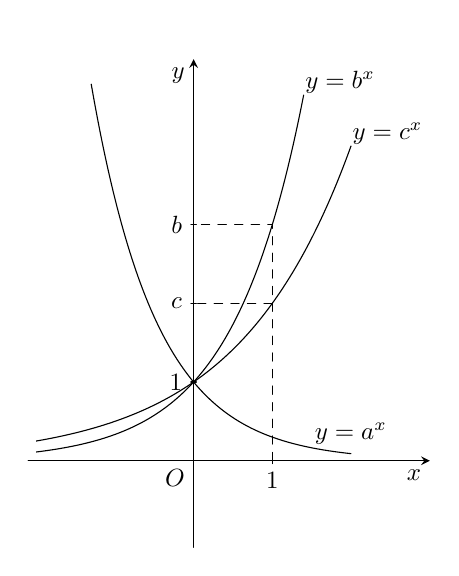
\begin{tikzpicture}[line join=round,line cap=round,>=stealth]
				\tikzset{every node/.style={scale=0.9}} 
				 \draw[->] (-2.1,0)--(3,0) node[below left] {$x$};
				\draw[->]  (0,-1.1)--(0,5.1) node[below left] {$y$};
				\draw (0,0) node [below left]  {$O$};
				\foreach \x/\nx  in {1/1}
				\draw[thin] (\x,1pt)--(\x,-1pt) node  [below] {$\nx$};
				\foreach \y/\ny  in {1/1,2/c,3/b}
				\draw[thin] (1pt,\y)--(-1pt,\y)  node [left] {$\ny$};
				 \draw[dashed,thin](1,2)--(0,2);
				\draw[dashed,thin](1,0)--(1,3)--(0,3); 
				\begin{scope}
					\clip (-2,-1)  rectangle (3,5.5);
					 \draw[samples=200,domain=-1.3:2,smooth,variable=\x] plot (\x,{0.3^(\x)}) node[above]{$y=a^x$};
					\draw[samples=200,domain=-2:1.4,smooth,variable=\x] plot (\x,{3^(\x)})  node[above right=-0.1cm]{$y=b^x$};
					 \draw[samples=200,domain=-2:2,smooth,variable=\x] plot (\x,{2^(\x)}) node[above right=-0.1cm]{$y=c^x$};
				\end{scope}
			\end{tikzpicture}
	\end{center}
	 \choice
		 {$a<b<c$}
		 {$b<c<a$}
		{$c<a<b$} 
		{\True  $a<c<b$}
	 \loigiai{
		Dựa vào đồ thị,  dễ thấy $\heva{&0<a<1\\&b,c>1.}$\\
		Đường thẳng  $x=1$ cắt hai đồ thị $y=b^x$, $y=c^x$ lần lượt tại $b$, $c$ và ta thấy $b>c$.\\
		Vậy $a<c<b$. 
	} 
\end{ex}

% từ: cau-hoi/lop11/1D6_Ham_so_mu_va_ham_so_logarit/1D6-3-3_Su_bien_thien_va_do_thi_cua_ham_so_mu_logarit.tex
\begin{ex}%[1D6V3-3]%[ma:6c39dc52]
	Biết hàm số $f(x)=\dfrac{a}{b^2\cdot 3^x}$ có đồ thị đối xứng với đồ thị hàm số $y=3^x$ qua  đường thẳng $x=-1$. Biết $a$, $b$ là các số nguyên. Chọn khẳng định đúng trong các khẳng định sau:
	\begin{center}
		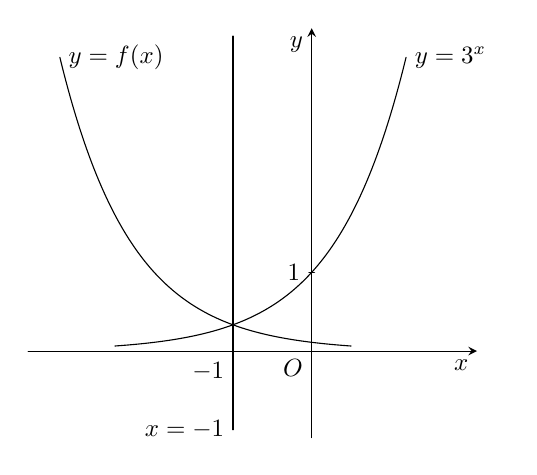
\begin{tikzpicture}[line join=round,line cap=round,>=stealth]
				\tikzset{every  node/.style={scale=0.9}}
				\draw[->] (-3.6,0)--(2.1,0)  node[below left] {$x$};
				\draw[->] (0,-1.1)--(0,4.1) node[below  left] {$y$};
				\draw (0,0)  node [below left] {$O$};
				\foreach \x/\nx in {-1/-1} 
				\draw[thin] (\x,1pt)--(\x,-1pt) node [below left] {$\nx$}; 
				\foreach \y/\ny in {1/1} 
				 \draw[thin] (1pt,\y)--(-1pt,\y) node [left] {$\ny$};
				\begin{scope}
					\clip (-3.5,-1) rectangle  (2.5,4);
					\draw[samples=200,domain=-2.5:1.2,smooth,variable=\x]  plot (\x,{3^(\x)}) node[right]{$y=3^x$};
					 \draw[samples=200,domain=0.5:-3.2,smooth,variable=\x] plot (\x,{1/(3^((\x)+2))}) node[right]{$y=f (x)$};
				\end{scope}
				 \draw (-1,4)--(-1,-1) node[left]{$x=-1$};
			\end{tikzpicture}
	\end{center}
	 \choice
		{\True  $b^2=9a$}
		{$b^2=4a$} 
		{$b^2=6a$} 
		 {$b^2=a$}
	 \loigiai{
		\begin{center}
			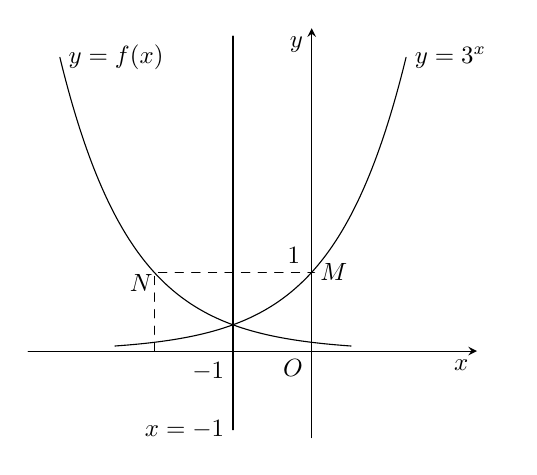
\begin{tikzpicture}[line join=round,line cap=round,>=stealth]
					\tikzset{every node/.style={scale=0.9}} 
					\draw[->] (-3.6,0)--(2.1,0) node[below  left] {$x$};
					\draw[->]  (0,-1.1)--(0,4.1) node[below left] {$y$};
					\draw (0,0) node [below left]  {$O$};
					 \foreach \x/\nx in {-1/-1}
					\draw[thin]  (\x,1pt)--(\x,-1pt) node [below left] {$\nx$};
					\foreach \y/\ny  in {1/1}
					\draw[thin] (1pt,\y)--(-1pt,\y) node [above  left] {$\ny$};
					\begin{scope}
						\clip (-3.5,-1) rectangle (2.5,4); 
						\draw[samples=200,domain=-2.5:1.2,smooth,variable=\x] plot  (\x,{3^(\x)}) node[right]{$y=3^x$};
						\draw[samples=200,domain=0.5:-3.2,smooth,variable=\x] plot  (\x,{1/(3^((\x)+2))}) node[right]{$y=f (x)$};
					\end{scope}
					\draw  (-1,4)--(-1,-1) node[left]{$x=-1$};
					\draw[dashed](-2,0)--(-2,1)--(0,1); 
					\node[right]  at (0,1) {$M$};
					 \node[below left=-0.1cm] at (-2,1) {$N$};
				\end{tikzpicture}
		\end{center}
		Trên đồ thị hàm số $y=3^x$ lấy $M(x_0;y_0)$ và gọi $N\Big(x,f(x)\Big)$ là điểm thuộc đồ thị hàm số $f(x)$ và đối xứng với $M$ qua đường thẳng  $x=-1$.\\
		 Khi đó $\heva{&\dfrac{x+x_0}{2}=-1\\&f(x)=y_0}\Leftrightarrow \heva{&x_0=-x-2\\&y_0=f(x).}$\\
		 Thay vào hàm số $y=3^x$ ta được $f(x)=3^{-x-2}=\dfrac{1}{3^23^x}$.\\
		Vậy $a=1$;  $b=3\Rightarrow b^2=9a$.
	} 
\end{ex}

% từ: cau-hoi/lop11/1D6_Ham_so_mu_va_ham_so_logarit/1D6-3-3_Su_bien_thien_va_do_thi_cua_ham_so_mu_logarit.tex
\begin{ex}%[1D6N3-3]%[ma:eba81fbd]
 Xét tính đúng sai của các mệnh đề  sau
 \choiceTF 
  {Hàm số $y=a^x$ với $a>1$ nghịch biến trên khoảng $\left(-\infty;+\infty  \right)$}
  {\True Hàm số $y=a^x$ với $0<a<0{,}5$ nghịch  biến trên khoảng $(-\infty;+\infty)$}
   {\True Hàm số $y=\log_{a}x$ với $a>1$ đồng biến trên khoảng $(0;+\infty)$}
  {Hàm số $y=\log_{a}x$ với $0<a<1$ nghịch biến trên khoảng  $(-\infty;+\infty)$}
  \loigiai{
 Xét  hàm số $y=a^x$.
 \begin{itemize}
  \item Khi $0<a<1$ thì hàm số $y=a^x$ nghịch biến trên  $\mathbb{R}$.
  \item Khi $a>1$ thì hàm số  $y=a^x$ đồng biến trên $\mathbb{R}$.
 \end{itemize}
 Xét hàm  số $y=\log_{a}x$.
 \begin{itemize}
  \item Khi  $0<a<1$ thì hàm số $y=\log_{a}x$ nghịch biến trên $(0;+\infty)$.
  \item  Khi $a>1$ thì hàm số $y=\log_{a}x$ đồng biến trên $(0;+\infty)$.
 \end{itemize}
  }
\end{ex}

% từ: cau-hoi/lop11/1D6_Ham_so_mu_va_ham_so_logarit/1D6-3-4_So_sanh_cac_luy_thua_va_logarit.tex
\begin{ex}%[1D6N3-4]%[ma:81e78a6c]
 Với $a$, $b$ là các số thực dương bất kì. Xét  tính đúng sai của các mệnh đề sau
 \choiceTF 
  {$\log_{\tfrac{1}{5}}a>\log_{\tfrac{1}{5}}b\Leftrightarrow  a>b$}
  {$\log (3a)<0$} 
  {\True $\log_{5}a>1\Leftrightarrow  a>5$}
  {\True  $\log_{2024}a^3=3\log_{2024}a$}
 \loigiai{ 
 \begin{itemchoice}
  \itemch Vì $\dfrac{1}{5}\in (0;1)$ nên $\log_{\tfrac{1}{5}}a>\log_{\tfrac{1}{5}}b\Leftrightarrow a<b\,\,\,\forall  a,b\in\mathbb{R}^+$.
  \itemch $a>0\Rightarrow 3a>0\Rightarrow \log (3a) >\log 0\Rightarrow\log (3a)>1$. 
  \itemch Vì $5>1$ nên  $\log_{5}a>1\Leftrightarrow a>5$.
  \itemch Áp dụng  công thức $\log_{a}b^M=M\log_{a}b$, ta có $\log_{2024}a^3=3\log_{2024}a$.
 \end{itemchoice}
  }
\end{ex}

% từ: cau-hoi/lop11/1D6_Ham_so_mu_va_ham_so_logarit/1D6-4-1_Dieu_kien_co_nghiem.tex
\begin{ex}%[1D6V4-1]%[ma:42215ce3]
	Tìm $m$ để phương trình $m\cdot2^{x^2-5x+6}+2^{1-x^2}=2\cdot2^{6-5x}+m\; \;  (1)$ có $4$ nghiệm phân biệt.
	\loigiai{ 
		Ta có 
		\begin{eqnarray*}
			m\cdot 2^{x^2-5x+6}+2^{1-x^2}=2^{7-5x}+m &\Leftrightarrow & m\cdot 2^{x^2-5x+6}+2^{1-x^2}=2^{\left(x^2-5x+6\right)+\left(1-x^2\right)}+m\\ 
			 &\Leftrightarrow & m\cdot2^{x^2-5x+6}+2^{1-x^2}=2^{x^2-5x+6}\cdot 2^{1-x^2}+m\\
			&\Leftrightarrow &  \left(2^{x^2-5x+6}-1\right)\left(2^{1-x^2}-m\right)=0\\
			&\Leftrightarrow & \hoac{&2^{x^2-5x+6}=1 \\  &2^{1-x^2}=m}\\
			&\Leftrightarrow  & \hoac{&x=3 \\&x=2 \\&2^{1-x^2}=m. \qquad (*)}
		\end{eqnarray*}
		Phương trình $(*)\Leftrightarrow \heva{&m > 0\\&1-x^2=\log_2m} \Leftrightarrow \heva{&m > 0\\ &x^2=1-\log_2m.}$\\ 
		$(1)$ có $4$ nghiệm phân biệt $\Leftrightarrow (*)$ có $2$ nghiệm phân biệt khác $2$ và  $3$.
		\[\Leftrightarrow  \heva{&{m > 0} \\
		&{1-\log_2m > 0}  \\
		 &{1-\log_2m\ne 4} \\
		 &{1-\log_2m\ne 9}
		} \Leftrightarrow  \heva{&{m > 0} \\
		&{m < 2} \\ 
		 &{m\ne \dfrac{1}{8}} \\
		&{m\ne \dfrac{1}{256}} 
		} \Leftrightarrow m\in \left(0;2\right)\setminus \left\{\dfrac{1}{8};\dfrac{1}{256} \right\}. 
		 \]
	} 
\end{ex}

% từ: cau-hoi/lop11/1D6_Ham_so_mu_va_ham_so_logarit/1D6-4-2_Phuong_trinh_mu_logarit_co_ban.tex
\begin{bt}%[1D6H4-2]%[ma:5809c54e]
% nguon: Archive/2024/TOAN_11_XE/TOAN_11_XE/data4/11C6/KNTT-6.4.tex #1014
%[TeX hóa SGK 11 - CTST - Đoàn Mạnh Hùng]
	Giải các phương trình sau
	\begin{listEX}[3]
		\item $3^{x+2}=\sqrt[3]{9}$.
		\item $2\cdot 10^{2 x}=30$.
		\item $4^{2 x}=8^{2 x-1}$.
	\end{listEX}
	\loigiai{
		\begin{listEX}
			\item $3^{x+2}=\sqrt[3]{9}\Leftrightarrow x+2=\dfrac{2}{3}\Leftrightarrow x=-\dfrac{4}{3}$.
			\item $2\cdot 10^{2 x}=30\Leftrightarrow x=\dfrac{1}{2}\log_{10} 15$.
			\item $4^{2 x}=8^{2 x-1}\Leftrightarrow 2^{4x}=2^{6x-3}\Leftrightarrow x=\dfrac{3}{2}$.
		\end{listEX}
	}
\end{bt}

% từ: cau-hoi/lop11/1D6_Ham_so_mu_va_ham_so_logarit/1D6-4-3_Bat_phuong_trinh_mu_logarit_co_ban.tex
\begin{bt}%[1D6H4-3]%[ma:b04180fc]
	 Giải bất phương trình sau $3^{x^{2}-4x+5} > \dfrac{1}{9}$.
	\loigiai{Ta  có
		\begin{eqnarray*}
			3^{x^2-4x+5} > \dfrac{1}{9} \Leftrightarrow 3^{x^2-4x+5} > 3^{-2} \Leftrightarrow x^2-4x+5 >-2 ~(\text{do}~3 > 1)\Leftrightarrow x^2-4x+7  > 0\Leftrightarrow x\in \mathbb{R}.
		\end{eqnarray*}
	Vậy nghiệm của bất  phương trình là $x\in \mathbb{R}$.}
\end{bt}

% từ: cau-hoi/lop11/1D6_Ham_so_mu_va_ham_so_logarit/1D6-4-4_Phuong_trinh_mu_logarit_dua_ve_cung_co_so.tex
\begin{ex}%[1D6V4-4]%[ma:b3b5045d]
 Cho phương trình $\log_3 \left(3^x-1\right)\cdot\log _{27} \left(3^{x+2}-9\right)=m$ với $m$ là tham số. Xét tính đúng sai của  các mệnh đề sau.
 \choiceTF 
  {Điều kiện xác định của phương trình  là $x\ge 0$}
  {Khi $m=1$  phương trình có một nghiệm là $x=\log_3 2$}
  {\True Đặt $\log_3 \left(3^x-1\right)=t$. Khi đó phương trình đã cho trở thành $t^2+2t-3m=0$} 
  {\True Phương trình đã cho có hai  nghiệm phân biệt khi và chỉ khi $m >-\dfrac{1}{3}$}
 \loigiai{ 
  \begin{itemchoice}
   \itemch Sai. Điều kiện xác định $\heva{&{3^x-1> 0}  \\
   &{3^{x+2}-9> 0} 
    &}$ $\Leftrightarrow$ $x > 0$.
    \itemch Sai. Khi $m=1$ phương trình có dạng
   \begin{eqnarray*}
    \log_3\left(3^x-1\right)\cdot\log _{27} \left(3^{x+2}-9\right)=1&\Leftrightarrow& \log_3\left(3^x-1\right)\cdot\log _{3^3} \left[3^2\left(3^x-1\right)\right]=1\\ 
    &\Leftrightarrow&  \log_3\left(3^x-1\right)\cdot\left[\log_3\left(3^x-1\right)+2\right]=3\\
     &\Leftrightarrow& \left[\log_3\left(3^x-1\right)\right]^2+2\log_3\left(3^x-1\right)-3=0\\
    &\Leftrightarrow& \hoac{&{\log_3\left(3^x-1\right)=1}  \\
     &{\log_3\left(3^x-1\right)=-3}
    &}  \Leftrightarrow \hoac{&{3^x-1=3} \\
    &{3^x-1=\dfrac{1}{27}} 
     &}\\
    &\Leftrightarrow& \hoac{&{3^x=4}  \\
    &{3^x=\dfrac{28}{27}} 
     &}\Leftrightarrow \hoac{&{x=\log_34} \\
    &{x=\log_3\dfrac{28}{27}} 
    &}  \Leftrightarrow \hoac{&{x=2\log_32} \\
     &{x=\log_3\dfrac{28}{27}.}
    &} 
   \end{eqnarray*}
   \itemch Đúng. 
   \begin{eqnarray*}
    \log_3\left(3^x-1\right)\cdot\log _{27}  \left(3^{x+2}-9\right)=m&\Leftrightarrow& \log_3\left(3^x-1\right)\cdot\log _{3^3} \left[3^2\left(3^x-1\right)\right]=m\\
    &\Leftrightarrow& \log_3\left(3^x-1\right)\cdot\left[\log_3\left(3^x-1\right)+2\right]=3m\\ 
    &\Leftrightarrow&  \left[\log_3\left(3^x-1\right)\right]^2+2\log_3\left(3^x-1\right)-3m=0.
   \end{eqnarray*}
   Khi đó đặt  $\log_3\left(3^x-1\right)=t$ thì phương trình đã cho trở thành $t^2+2t-3m=0$.\tagEX{1}
   \itemch Đúng. Phương trình đã cho có hai nghiệm  phân biệt khi và chỉ khi phương trình $(1)$ có hai nghiệm phân biệt $\Leftrightarrow$ $\Delta '=1+3m > 0$ $\Leftrightarrow$ $m >-\dfrac{1}{3}$.
  \end{itemchoice}
  }
\end{ex}

% từ: cau-hoi/lop11/1D6_Ham_so_mu_va_ham_so_logarit/1D6-4-4_Phuong_trinh_mu_logarit_dua_ve_cung_co_so.tex
\begin{ex}%[1D6V4-4]%[ma:cca90bea]
	Cho  phương trình $9^x-2\cdot 3^{x+1}+m=0$ với $m$ là tham số thực.
	\choiceTF 
		{\True Với $m=9$ thì  phương trình đã cho có cùng tập nghiệm với phương trình\\ $4^x-2^x-2=0$}
		{Phương trình có hai nghiệm phân biệt khi $m  < 9$}
		{Phương trình có hai  nghiệm phân biệt trái dấu khi và chỉ khi $m < 0$}
		{\True Gọi $m_0$ là giá trị mà  phương trình có hai nghiệm phân biệt $x_1$, $x_2$ thỏa mãn\\ $x_1+x_2=1$. Khi đó $m_0 \in (2;6)$}
	 \loigiai{
		\begin{itemchoice}
			 \itemch
			Theo đề ta có phương trình $9^x-2\cdot  3^{x+1}+m=0. \quad(1)$\\
			 Ta có
			\begin{eqnarray*}
				&&4^x-2^x-2=0\quad(2) \\ 
				 &\Leftrightarrow & \left(2^x \right)^2-2^x-2=0\\
				&\Leftrightarrow  &\hoac{& 2^x=-1\\& 2^x=2.}
			\end{eqnarray*}
			\begin{itemize}
				\item Với $2^x=-1$ vô nghiệm. 
				 \item Với $2^x=2\Leftrightarrow x=1$.
				\item Vậy nghiệm của phương trình  $(2)$ là $x=1$.
			\end{itemize}
			Với $m=9$, thế vào $(1)$ ta  có
			\begin{eqnarray*}
				 && 9^x-2\cdot 3^{x+1}+9=0\\
				 &\Leftrightarrow &\left(3^x \right)^2-6\cdot 3^x+9=0\\
				&\Leftrightarrow  & \left(3^x-3\right)^2=0\Leftrightarrow 3^x=3\Leftrightarrow x=1.
			\end{eqnarray*}
			Vậy khi $m=9$ thì hai phương trình có chung tập  nghiệm.
			\itemch 
			Theo đề ta có phương trình $9^x-2\cdot 3^{x+1}+m=0$ $\Leftrightarrow \left(3^x \right)^2-6.3^x+m=0.\quad  (1)$\\
			Đặt $t=3^x$, với $t > 0$. 
			Khi đó phương  trình $(1)$ trở thành $t^2-6t+m=0.\quad(3)$\\
			Phương trình $(1)$ có hai nghiệm phân biệt $\Leftrightarrow (3)$ có hai nghiệm phân  biệt dương
			\[\Leftrightarrow \heva{&\Delta '=9-m > 0\\& S=6> 0\\&P=m > 0} \Leftrightarrow  0< m < 9.\]
			 \itemch
			Dựa vào ý trên, ta có  phương trình $(1)$ có $2$ nghiệm phân biệt khi $0< m < 9\quad (*)$.\\
			Phương trình $(1)$ có hai nghiệm  phân biệt $x_1$, $x_2$ thỏa $x_1 < 0< x_2$
			\begin{eqnarray*}
				 &\Leftrightarrow & 0< 3^{x_1} < 3^0< 3^{x_2}\\
				&\Leftrightarrow & 0< t_1 < 1<  t_2\\
				t_1  < 1< t_2 &\Rightarrow & \left(t_1-1\right)\left(t_2-1\right) < 0\\
				&\Leftrightarrow & t_1 t_2-\left(t_1+t_2  \right)+1< 0\\
				m-6+1< 0\Leftrightarrow  m < 5.
			\end{eqnarray*}
			So với điều kiện $(*)$, ta có giá trị cần tìm là $0<  m < 5$.
			\itemch 
			Theo  đề ta có phương trình $9^x-2\cdot 3^{x+1}+m=0$ $\Leftrightarrow \left(3^x \right)^2-6.3^x+m=0.\quad(1)$ \\
			Đặt $t=3^x$, với $t >  0$.\\
			Khi đó phương trình $(1)$ trở thành  $t^2-6t+m=0.\quad(3)$\\
			Theo ý b, phương trình $(1)$ có $2$ nghiệm phân biệt $x_1$, $x_2$ khi  $0< m < 9\quad(*)$\\
			Theo đề  ta có
			\begin{eqnarray*}
				x_1+x_2=1 &\Leftrightarrow  &3^{x_1+x_2}=3^1\\
				&\Leftrightarrow & 3^{x_1}\cdot 3^{x_2}=3\\ 
				&\Leftrightarrow & t_1\cdot t_2=3\Leftrightarrow m=3~ \text{thỏa}~  (*).\\
			\end{eqnarray*}
			Vậy  $m_0=3\Rightarrow m_0 \in (2;6)$.
		\end{itemchoice}
	 }
\end{ex}

% từ: cau-hoi/lop11/1D6_Ham_so_mu_va_ham_so_logarit/1D6-4-4_Phuong_trinh_mu_logarit_dua_ve_cung_co_so.tex
\begin{ex}%[1D6C4-4]%[ma:41bbad6f]
	Cho $x$, $y$ là các số thực dương thỏa mãn $\log_{\sqrt{2(x+2y+2)}}\left(x^2+y^2\right)\leq 2$. Giá trị nhỏ nhất  của biểu thức $P=4x+3y+1$ bằng
	\shortans{-4} 
	\loigiai{ 
		Với $x$, $y$ là các số thực dương,  ta có $\sqrt{2(x+2y+2)}>1$. Do đó.\\
		$\log_{\sqrt{2(x+2y+2)}}\left(x^2+y^2\right)\leq  2\Leftrightarrow x^2+y^2\leq 2(x+2y+2)\Leftrightarrow(x-1)^2+(y-2)^2\leq 9\quad(C)$.\\
		Hình tròn  $(C)$ có tâm $I(1;2)$, bán kính $R=3$.\\
		Theo  giả thiết $P=4x+3y+1\Leftrightarrow 4x+3y+1-P=0\quad (d)$.\\
		Đường thẳng $(d)$  cắt hình tròn $(C)$ khi và chỉ khi $$\mathrm{d}(I,d)\leq R\Leftrightarrow\dfrac{|11-P|}{5}\leq 3\Leftrightarrow-4\leq P\leq 26.$$
	Vậy $\min  P=-4$.}
\end{ex}

% từ: cau-hoi/lop11/1D6_Ham_so_mu_va_ham_so_logarit/1D6-4-4_Phuong_trinh_mu_logarit_dua_ve_cung_co_so.tex
\begin{bt}%[1D6H4-4]%[ma:38d3b369]
	Giải bất phương  trình $3^{x^3-4x+5}>\dfrac{1}{9}$.
	\loigiai{ 
		 Ta có
		\begin{eqnarray*}
			 3^{x^3-4x+5}>\dfrac{1}{9}&\Leftrightarrow&3^{x^3-4x+5}>3^{-2}\\
			&\Leftrightarrow& x^2-4x+5>-2  (\text{ do} 3>1)\\
			&\Leftrightarrow&  x^2-4x+7>0\\
			&\Leftrightarrow&  x\in\mathbb{R}.
		\end{eqnarray*}
		Vậy nghiệm của bất phương  trình là $x\in\mathbb{R}$.
	} 
\end{bt}

% từ: cau-hoi/lop11/1D6_Ham_so_mu_va_ham_so_logarit/1D6-4-5_Bat_phuong_trinh_mu_logarit_dua_ve_cung_co_so.tex
\begin{bt}%[1D6H4-5]%[ma:9bf48828]
	Giải bất phương trình  $3^{4-x^2}\ge 27$.
	 \loigiai{
	$$3^{4-x^2}\ge 27\Leftrightarrow 3^{4-x^2}\ge  3^3\Leftrightarrow 4-x^2\ge 3\Leftrightarrow -1\le x\le 1 .$$
	} 
\end{bt}

% từ: cau-hoi/lop11/1D7_Dao_ham/1D7-1-5_Toan_thuc_te_khac_ap_dung_dinh_nghia_dao_ham.tex
\begin{bt}%[1D7C1-5]%[ma:5aa9eca0]
% nguon: Archive/SP_KhoLatex/SP_Đề Theo Bài-Khối 11/1-B31.tex #3926

	Người ta xây dựng một cây cầu vượt giao thông hình parabol nối hai điểm có khoảng cách là $400$ m. Độ dốc của mặt cầu không vượt quá $10^\circ$ (độ dốc tại một điểm được xác định bởi góc giữa phương tiếp xúc với mặt cầu và phương ngang). Tính chiều cao giới hạn từ đỉnh cầu đến mặt đường (làm tròn kết quả đến chữ số thập phân thứ nhất).\\
\begin{center}\begin{tikzpicture}[scale=1.5, font=\footnotesize, line join=round, line cap=round,>=stealth]
\draw[smooth,samples=100,domain=-2:2] plot(\x,{-0.25*(\x)^2});
\draw[smooth,samples=100,domain=-1.7:-0.3] plot(\x,{-0.5*(-1.2)*(\x+1.2)-0.36});
\draw (-2,-1)--(2,-1)node[below,pos=0.5]{$400$ m};
\path (-1.2,-0.36) coordinate (P) (-0.6,0) coordinate (a) (0,-0.36) coordinate (J);
\draw[dashed] (P)--(-0.5,-0.36) (0,-1)--(0,0)node[right,pos=0.5]{$?$};
\foreach \x/\y/\l/\g  in {-2/-1/A/-90,2/-1/B/-90,-1.2/-0.36/P/150}{\fill[black] (\x,\y) circle(1pt)+(\g:0.2) node{$\l$};}
\draw pic[draw, angle eccentricity=1.2, angle radius=0.5cm]{angle=J--P--a};
\end{tikzpicture}\end{center}
\shortans{$17{,}6$}
\loigiai{
\begin{center}
\begin{tikzpicture}[scale=1.5, font=\footnotesize, line join=round, line cap=round,>=stealth]
\def \xmin{-2.5};
\def \xmax{2.7};
\def \ymin{-1.5};
\def \ymax{1.0};
\draw[->] (\xmin, 0.) -- (\xmax,0.) node[anchor=north] {$x$};
\draw[->] (0.,\ymin) -- (0.,\ymax) node[anchor=west] {$y$};
\clip(\xmin+0.1,\ymin+0.1) rectangle (\xmax-0.1,\ymax-0.1);
\draw[smooth,samples=100,domain=-2:2] plot(\x,{-0.25*(\x)^2});
\draw[smooth,samples=100,domain=-1.7:-0.3] plot(\x,{-0.5*(-1.2)*(\x+1.2)-0.36});
\draw[dashed] (-2,0) node[above]{$-200$} |- (0,-1)node[]{}-|(2,0)node[above]{$200$} (-1.2,-0.36)--(-0.5,-0.36);
\path (-1.2,-0.36) coordinate (P) (-0.6,0) coordinate (a) (0,-0.36) coordinate (J);
\foreach \x/\y/\l/\g  in {0/0/O/45,-2/-1/A/-90,2/-1/B/-90,-1.2/-0.36/P/150,0/-1/I/-45}{\fill[black] (\x,\y) circle(1pt)+(\g:0.2) node{$\l$};}
\draw pic[draw, angle eccentricity=1.2, angle radius=0.5cm]{angle=J--P--a};
\end{tikzpicture}
\end{center}
Chọn hệ trục toạ độ như hình vẽ, sao cho đỉnh cầu là gốc tọa độ và mặt cắt của cây cầu có hình dạng parabol $y=-a x^2$ (với $a$ là hằng số dương).\\
Hệ số góc của tiếp tuyến của parabol bằng $k=y'(x_0)=-2 a x_0,-200 \leq x_0 \leq 200$.\\
Hệ số góc xác định độ dốc của mặt cầu (độ dốc dương) là $|k|=2 a|x| \leq 400 a$.\\
Vì độ dốc của mặt cầu không vượt quá $10^\circ$ nên ta có
$400 a \leq \tan 10^\circ \Leftrightarrow a \leq \dfrac{\tan 10^\circ}{400}$.\\
Chiều cao giới hạn từ đỉnh cầu đến mặt đường là đoạn $O I$, cũng chính là độ lớn của tung độ điểm $B$ khi $a$ đạt giá trị lớn nhất.\\
Do đó, $O I=\left|-a \cdot 200^2\right|\approx 17{,}6$ (m).\\
Vậy chiều cao giới hạn từ đỉnh cầu đến mặt đường là $17{,}6$ m.
}
\end{bt}

% từ: cau-hoi/lop11/1D7_Dao_ham/1D7-2-1_Tinh_dao_ham.tex
\begin{ex}%[1D7V2-1]%[ma:685247e5]
	Có bao nhiêu giá trị nguyên của tham số $m$ để bất phương trình $f'(x)\leq 0$ có tập nghiệm là $\mathbb{R}$, biết $f(x) =  -\dfrac{mx^3}{3}+\dfrac{mx^2}{2}-(3-m)x+2$?
	 \shortans{3}
	\loigiai{ 
	Ta có $f'(x) = -mx^2 + mx + m  - 3$.\\
	Với $f'(x) \leq 0$ ta  được bất phương trình $-mx^2 + mx + m - 3 \leq 0$. \hfill $(*)$
	\begin{itemize}
		\item Khi $m = 0$, bất phương trình $(*)$ nghiệm đúng với mọi $x$ thuộc $\mathbb{R}$. Vậy $m  = 0$ thỏa mãn yêu cầu bài toán.
		\item Khi $m \neq 0$ thì bất phương trình $(*)$ là một bất phương trình trình bậc hai ẩn $x$. Do đó $(*)$ có tập nghiệm là  $\mathbb{R}$ khi và chỉ khi
		\begin{align*}
			\heva{& -m<0 \\& m^2+4m(m-3)\leq 0}\Leftrightarrow \heva{& m>0 \\& 5m^2 - 12m \leq 0} \Leftrightarrow \heva{& m>0  \\& 0 \leq m \leq \dfrac{12}{5}} \Leftrightarrow 0<m \leq \dfrac{12}{5}.
		\end{align*}
	\end{itemize}
	Kết hợp hai trường hợp ta được $m \in \left[0;\dfrac{12}{5}\right]$. Vậy có $3$ giá trị nguyên của $m$ thỏa mãn đề  bài là $
	\{0; 1;  2\}$.
	 }
\end{ex}

% từ: cau-hoi/lop11/1D7_Dao_ham/1D7-2-1_Tinh_dao_ham.tex
\begin{bt}%[1D7V2-1]%[ma:37ca0620]
% nguon: Archive/SP_KhoLatex/ID6_old/16-OT-DaoHam-CongThucTinhDaoHam.tex #3822
%[ĐGNL-7-Nguyễn Thành Nhân]
	Cho hàm số $y=x^3-3mx^2+3\left(m^2-1\right)x$. Tìm tham số $m$ để phương trình $y'=0$ có hai nghiệm $x_1$, $x_2$ phân biệt thỏa mãn $x_1^2+x_2^2-x_1x_2=10$.
	\loigiai
	{Ta có $y'=3x^2-6mx+3\left(m^2-1\right)$ và $$y'=0\Leftrightarrow 3x^2-6mx+3\left(m^2-1\right)=0\Leftrightarrow x^2-2mx+m^2-1=0\quad (*).$$
		Ta biến đổi được $x_1^2+x_2^2-x_1x_2=10\Leftrightarrow \left(x_1+x_2\right)^2-3x_1x_2=10$.\\
		Khi đó, yêu cầu bài toán tương đương với
		\begin{eqnarray*}
			\heva{& \Delta' >0 \\ & S^2-3P=10}\Leftrightarrow\heva{& m^2-\left(m^2-1\right)>0 \\ & (2m)^2-3\left(m^2-1\right)=10}\Leftrightarrow m^2=7\Leftrightarrow m=\pm\sqrt{7}.
		\end{eqnarray*}
		Vậy giá trị $m$ cần tìm là $m=\pm\sqrt{7}$.
	}
\end{bt}

% từ: cau-hoi/lop11/1D7_Dao_ham/1D7-2-1_Tinh_dao_ham.tex
\begin{bt}%[1D7H2-1]%[ma:17bf06c0]
% nguon: Archive/SP_KhoLatex/ID6_old/16-OT-DaoHam-CongThucTinhDaoHam.tex #3829
%[ĐGNL, Nguyễn Thành Nhân]
	Cho hàm số $f(x)=\sin 2x-2\cos x$. Giải phương trình $f'(x)=0$.
	\loigiai
	{
		Ta có $f'(x)=2\cos 2x+2\sin x$. Khi đó
		\allowdisplaybreaks
		\begin{eqnarray*}
			f'(x)=0 
			\Leftrightarrow  2\cos 2x+2\sin x=0
			\Leftrightarrow -2\sin^2 x+\sin x+1=0
			\Leftrightarrow \left[\begin{aligned}&\sin x=1 \\&\sin x=-\dfrac{1}{2}\end{aligned}\right.
			\Leftrightarrow \hoac{&x=\dfrac{\pi}{2}+k2\pi\\&x=-\dfrac{\pi}{6}+k2\pi \\&x=\dfrac{7\pi}{6}+k2\pi},\,\,k\in \mathbb{Z}.
		\end{eqnarray*}
		Vậy phương trình $f'(x)=0$ có các nghiệm $x=\dfrac{\pi}{2}+k2\pi$, $x=-\dfrac{\pi}{6}+k2\pi$, $x=\dfrac{7\pi}{6}+k2\pi$ với $k\in \mathbb{Z}$.
	}
\end{bt}

% từ: cau-hoi/lop11/1D7_Dao_ham/1D7-2-6_Gioi_han_ham_so_luong_giac_ham_so_mu_logarit.tex
\begin{ex}%[1D7V2-6]%[ma:0987a4d4]
	Cho $ a \in \mathbb{N}^* $, $ a \le 9 $. Tìm giới hạn $A=\lim  \dfrac{a+\overline{aa}+\cdots+\underbrace{\overline{aa\ldots a}}_{ n \text{ chữ số } a}}{10^n}$.
	\loigiai{ Ta  có
	\begin{eqnarray*}
		& a+\overline{aa}+\cdots+\underbrace{\overline{aa\ldots a}}_{ n \text{ chữ số } a}&=a\cdot (1+11+111+\cdots+\underbrace{111  \ldots 1}_{n \text { chữ số } 1})\\
		& &=\dfrac{a}{9}\cdot (9+99+999+\ldots+\underbrace{999 \ldots  9}^{n \text { chữ số }9})\\
		 & & =\dfrac{a}{9}\cdot\left(10-1+10^2-1+10^3-1+\cdots+10^n-1\right)\\
		 & &=\dfrac{a}{9}\cdot\left[\dfrac{10\left(10^n-1\right)}{9}-n\right].
	\end{eqnarray*}
	Ta có $\lim \dfrac{a+\overline{aa}+\cdots+\underbrace{\overline{aa\ldots a}}_{ n \text{ chữ số } a}}{10^n}=\lim \dfrac{a}{9\cdot 10^n}\left[\dfrac{10\left(10^n-1\right)}{9}-n\right]=\lim \dfrac{a}{9}\left[\dfrac{10\left(10^n-1\right)}{9\cdot  10^n}-\dfrac{n}{10^n}\right]$.\\
	 Mặt khác $\lim \dfrac{10\left(10^n-1\right)}{9\cdot 10^n}=\dfrac{10}{9}$.\\
	 Và $n \leq \mathrm{C}_n^0+\mathrm{C}_n^1+\cdots+\mathrm{C}_n^n=2^n \Rightarrow 0 \leq \dfrac{n}{10^n} \leq\left(\dfrac{2}{10}\right)^n=\dfrac{1}{5^n}$, mà $\lim \dfrac{1}{5^n}=0 \Rightarrow \lim \dfrac{n}{10^n}=0$.\\
	 Vậy $A=\dfrac{10 a}{81}$.
	 }
\end{ex}

% từ: cau-hoi/lop11/1D7_Dao_ham/1D7-2-8_Toan_thuc_te_ap_dung_quy_tac_dao_ham.tex
\begin{ex}%[1D7V2-8]%[ma:235871af]
	Người ta xây một cây cầu vượt giao thông hình parabol nối hai điểm có khoảng cách là $400$ m (hình bên dưới). Độ dốc của mặt cầu không vượt quá $10^\circ$ (độ dốc tại một điểm được xác định bởi góc giữa phương tiếp xúc với mặt cầu và phương ngang như hình dưới đây). Tính chiều cao  giới hạn từ đỉnh cầu đến mặt đường (làm tròn kết quả đến chữ số thập phân thứ nhất).
	\begin{center}
		\begin{tikzpicture}[line join=round,line cap=round,line width=.6pt,font=\footnotesize,scale=1.2]
				\def\a{-1/8} 
				\def\b{0} 
				 \def\c{2}
				\draw[->] (-5,0) -- (5,0) node[below]  {$x$};
				\draw[->]  (0,-1) -- (0,3) node[left] {$y$};
				\draw (0,0)  node[below left]{$O$};
				\pgfmathsetmacro\xdinh{-(\b)/2*(\a)} 
				\pgfmathsetmacro\ydinh{(4*(\a)*(\c)-(\b)^2)/(4*(\a))} 
				\fill[black]  (\xdinh,\ydinh) node[shift={(120:8pt)}]{$h$} circle (2pt);
				\fill[black] (-4,0) node[shift={(120:8pt)}]{$A$} circle (2pt); 
				\fill[black] (4,0) node[shift={(60:8pt)}]{$B$} circle  (2pt);
				\draw[<->,dashed]  (-4,-0.5)--(0,-0.5) node[below,pos=0.5]{$ 200 $ m};
				\draw[<->,dashed] (0,-0.5)--(4,-0.5) node[below,pos=0.5]{$ 200  $ m};
				 \clip (-5,-1) rectangle (5,3);
				\draw[thick,samples=150,smooth,domain=-4:4]  plot (\x,{\a*(\x)^2+(\b)*\x+(\c)});
			\end{tikzpicture}
	\end{center}
	\shortans{17,6} 
	 \loigiai{
		Chọn hệ trục tọa độ $Oxy$ sao  cho $O$ là trung điểm $AB$. Tia $Ox$ trùng với tia $OB$, tia $Oy$ vuông góc với tia $Ox$ tại $O$.\\
		Khi đó ta  có $A\left(-200;0\right)$, $B\left(200;0\right)$.\\
		Gọi chiều  cao giới hạn của cầu là $h$ $\left(h > 0\right)$, suy ra đỉnh cầu có tọa độ $\left(0;h\right)$.\\
		Ta tìm được phương trình parabol của cầu là $y=-\dfrac{h}{200^2}{x^2}+h$.\\ 
		Ta có $y'=-\dfrac{2h}{200^2}x$.\\ 
		Suy ra  hệ số góc xác định độ dốc của mặt cầu là $k=y'=-\dfrac{2h}{200^2}x$ với $-200\le x\le 200$.\\
		Do đó, $\left| k\right|=\left|-\dfrac{2h}{200^2}x\right|=\dfrac{2h}{200^2}\cdot \left| x\right|\le\dfrac{2h}{200^2}\cdot 200=\dfrac{h}{100}$.\\ 
		Vì độ dốc của mặt cầu không quá  $10^\circ $ nên ta có $\dfrac{h}{100}\le\tan 10^\circ \Leftrightarrow h\le 17{,}6$.\\
	Vậy chiều cao giới hạn từ đỉnh  cầu tới mặt đường là $17{,}6$ m.}
\end{ex}

% từ: cau-hoi/lop11/1D7_Dao_ham/1D7-2-8_Toan_thuc_te_ap_dung_quy_tac_dao_ham.tex
\begin{bt}%[1D7H2-8]%[ma:9b0b2457]
% nguon: Archive/SP_DA_SauLuoi/1-TL-TN-THPT-Chuyen-LeQuyDon-NinhThuan-HKII-NH23-24.tex #2535
%[Dự án đề kiểm tra Toán 11 CKII NH23-24-Đợt 16-Lê Hữu Kiệt]%[THPT Chuyên Lê Quý Đôn- Ninh Thuận]
	\immini[thm]
	{Một vật chuyển động trong $4$ giờ với vận tốc $v$ phụ thuộc vào thời gian $t$ và có đồ thị vận tốc như hình bên. Trong khoảng thời gian $4$ giờ kể từ khi bắt đầu chuyển động, đồ thị đó là một phần của đường parabol có đỉnh $I\left( \dfrac{5}{2};\,-\dfrac{9}{4} \right)$ và có trục đối xứng song song trục tung. Tính gia tốc của vật lúc $t=3$ giờ.}
	{\begin{tikzpicture}[font=\footnotesize, >=stealth, x=0.6cm, y=0.6cm]
	\draw[->] (-0.5,0)--(6,0)node[above]{$t$ (giờ)};
	\draw[->] (0,-3)--(0,5)node[left]{$v$ (km/giờ)};
	\draw (0,0) node[below left]{$O$};
	\draw[dashed] (5/2,0) |- (0,-9/4);
	\begin{scope}
		\clip (-0.5,-3) rectangle (5.5,4.8);
		\draw[smooth] plot[domain=0:4] (\x,{(\x)^2-5*(\x)+4});
	\end{scope}
	\foreach \x in {(5/2,0), (0,4), (0,-9/4), (5/2,-9/4)}{\fill[black] \x circle (1pt);}
	\draw (0,4)node[left]{$4$} (0,-9/4)node[left]{$-\dfrac{9}{4}$} (5/2,0)node[above]{$\dfrac{5}{2}$} (5/2,-9/4)node[below]{$I$};
	\end{tikzpicture}}
	\loigiai{
	Gọi $v(t)=at^2+bt+c$ ($a> 0$) là hàm số vận tốc cần tìm (đơn vị: km/giờ). Ta có
	\begin{itemize}
		\item Đồ thị hàm số đi qua điểm $(0;\,4)$, suy ra $c=4$;
		\item Hoành độ đỉnh $I$ là $-\dfrac{b}{2a}=\dfrac{5}{2} \Leftrightarrow b=-5a$; \quad$(1)$
		\item Tung độ đỉnh $I$ là $-\dfrac{b^2-4ac}{4a}=-\dfrac{9}{4} \Leftrightarrow b^2-16a=9a \Leftrightarrow b^2-25a=0$. \quad$(2)$
	\end{itemize}
	Thay $(1)$ vào $(2)$ ta được
	\allowdisplaybreaks
	\begin{eqnarray*}
		&& (-5a)^2-25a=0 \\
		&& 25a^2-25a=0 \\
		&& a=1 \quad\text{hoặc} \quad a=0.
	\end{eqnarray*}
	Vì $a>0$ nên ta nhận $a=1$. Khi đó $b=-5\cdot1=-5$.\\
	Suy ra $v(t)=t^2-5t+4$.\\
	Gọi $a(t)$ là gia tốc của vật (đơn vị: km/giờ$^2$), ta có $a(t)=v'(t)=2t-5$.\\
	Khi đó, gia tốc của vật lúc $t=3$ giờ là $a(3)=1$ (km/giờ$^2$).
	}
\end{bt}

% từ: cau-hoi/lop11/1D7_Dao_ham/1D7-2-8_Toan_thuc_te_ap_dung_quy_tac_dao_ham.tex
\begin{bt}%[1D7V2-8]%[ma:febd937f]
% nguon: Archive/SP_KhoLatex/SP_Đề Theo Bài-Khối 11/1-B32.tex #3966

Một vật chuyển động có phương trình $s(t)=4\cos \left(2\pi t-\dfrac{\pi}{8} \right)$ (m) với $t$ là thời gian tính bằng giây. Tính vận tốc của vật khi $t=5$ giây (làm tròn kết quả đến chữ số thập phân thứ nhất).
\shortans{$9{,}6$}
\loigiai{
Ta có $v(t)=s'(t)=-4\left(2\pi t-\dfrac{\pi}{8} \right)' \sin \left(2\pi t-\dfrac{\pi}{8} \right)=-8\pi \sin \left(2\pi t-\dfrac{\pi}{8} \right)$.\\
Vận tốc của vật khi $t=5$ giây là $v(5)=-8\pi \sin \left(2\pi\cdot 5-\dfrac{\pi}{8} \right)=8\pi \sin \dfrac{\pi}{8}\approx 9{,}6$ (m).
}
\end{bt}

% từ: cau-hoi/lop11/1D7_Dao_ham/1D7-3-1_Tinh_dao_ham_cap_hai.tex
\begin{bt}%[1D7H3-1]%[ma:bb6a3554]
% nguon: Archive/SP_DA_SauLuoi/1-TL-TN-DS-THPT-ChuyenTranPhu-HaiPhong-HKII-NH23-24.tex #2564
%[Dự án đề kiểm tra Toán 11 HK2 NH23-24 - Phan Anh]%[THPT Chuyên Trần Phú - Hải Phòng]
Cho hàm số $f(x)=\dfrac{x^2+x+1}{x+1}$. Tập nghiệm của bất phương trình $f''(x)>0$ có bao nhiêu giá trị nguyên dương $x\le2024$?
\loigiai{Ta có $f(x)=\dfrac{x^2+x+1}{x+1}=\dfrac{x(x+1)+1}{x+1}=x+\dfrac{1}{x+1}$, suy ra 
\[f'(x)=1-\dfrac{1}{(x+1)^2},\,f''(x)=\dfrac{2}{(x+1)^3}.\]
Do đó nên $f''(x)>0\Leftrightarrow\dfrac{2}{(x+1)^3}>0\Leftrightarrow x+1>0\Leftrightarrow x>-1$.\\
Do $x$ là số nguyên dương và $x\le2024$ nên $x\in\{1;2;\ldots;2024\}$.\\
Vậy có $2024$ giá trị $x$ thỏa mãn yêu cầu bài toán.}
\end{bt}

% từ: cau-hoi/lop11/1H8_Quan_he_vuong_goc_trong_khong_gian/1H8-1-3_Tim_goc_giua_hai_duong_thang.tex
\begin{ex}%[1H8V1-3]%[ma:1b2f549f]
	Cho hình chóp $S. A B C D$ có đáy là hình bình hành tâm $O$. Biết $\widehat{S A D}=\widehat{S C D}=90^{\circ}$. Tìm số đo  của góc $(S B, A C)$
	 \loigiai{
	\immini{ 
		Gọi $M$  là trung điểm cạnh $S D$.\\
		Khi đó $O M$ là đường trung bình của tam giác $S B D$ nên  $O M \parallel S B$.\\
		 Do vậy $(S B, A C)=(O M, A C)$.\\
		Tam giác $S A D$ vuông tại $A$  có trung tuyến $A M=\dfrac{S D}{2}$;\\
		Tam giác $S C D$ vuông tại  $C$ có trung tuyến $C M=\dfrac{S D}{2}$.\\
		Suy ra tam  giác $M A C$ cân tại $M$, mà $O$ là trung điểm $A C$ nên $O M \perp A C$ hay $(O M, A C)=90^{\circ}$. Do đó $(S B, A C)=90^{\circ}$ hay $S B \perp A C$.
		} 
		 {
		\begin{tikzpicture}[scale=0.9]
				 \tkzDefPoints{0/0/D,-2/-2/C,2.5/-2/B}
				\coordinate (A) at ($(B)+(D)-(C)$); 
				 \draw (C)--(B)--(A);
				 \draw[dashed] (C)--(D)--(A);
				\coordinate  (O) at ($(A)!0.5!(C)$);
				 \coordinate (S) at ($(O)+(-0.5,5)$);
				\coordinate  (M) at ($(S)!0.5!(A)$);
				 \draw[dashed] (O)--(S)--(D)--(B)
					 (A)--(C)
					(D)--(M)--(O); 
				\draw (S)--(A) 
					 (S)--(B)--(M)
					(S)--(C); 
				 \tkzMarkRightAngle (A,O,D)
				\tkzMarkRightAngle (S,D,A) 
				\tkzMarkRightAngle  (S,B,A)
				\begin{footnotesize}
					\draw (S)  node[above]{$S$};
					\draw (C)  node[left]{$B$};
					 \draw (D) node[left]{$A$};
					\draw (A)  node[right]{$D$};
					\draw  (B) node[right]{$C$};
					 \draw (M) node[right]{$M$};
					\draw (O) node[below]{$O$}; 
				\end{footnotesize}
			\end{tikzpicture}
		 }
	 }
\end{ex}

% từ: cau-hoi/lop12/2D1_Ung_dung_dao_ham_de_khao_sat_ham_so/2D1-2-2_Tim_cuc_tri_dua_vao_BBT_do_thi.tex
\begin{bt}%[2D1H2-2]%[ma:7664e335]
% nguon: Archive/2024/TaiLieuGiangDay/1.HamSo/1. K12 - 4in1 - Hamso/ThubaiGoc/Bai2-Dang2.tex #2622
%[BG12, Tran Tony]
	\immini{
		Cho hàm số $y=\dfrac{ax^2+bx+c}{dx+e}$ có đồ thị $(C)$ như hình vẽ bên. Viết phương trình đường thẳng đi qua hai điểm cực trị của đồ thị $(C)$.
	}{
		\begin{tikzpicture}[scale=0.6, font=\footnotesize, line join=round, line cap=round, >=stealth,yscale=0.7]
			\tikzset{every node/.style={scale=0.9}}
			\draw[->] (-3.6,0)--(5.6,0) node[below] {$x$};
			\draw[->] (0,-6.1)--(0,6.1) node[left] {$y$};
			\draw (0,0) node [below left] {$O$};
			\draw[thin] (-1,1pt)--(-1,-1pt) node [above] {$-1$};
			\draw[thin] (3,1pt)--(3,-1pt) node [below] {$3$};
			\draw[thin] (1pt,-4)--(-1pt,-4) node [right] {$-4$};
			\draw[thin] (1pt,4)--(-1pt,4) node [left] {$4$};
			\draw[dashed,thin](-1,0)--(-1,-4)--(0,-4);
			\draw[dashed,thin](3,0)--(3,4)--(0,4);
			\draw[dashed,thin] (1.01,-6)--(1.01,6);
			\begin{scope}
				\clip (-3.5,-6) rectangle (5.5,6);
				\draw[samples=200,domain=-3:0.99,smooth,variable=\x] plot (\x,{(1*((\x)^2)+-2*(\x)+5)/(1*(\x)+-1)});
				\draw[samples=200,domain=1.01:5,smooth,variable=\x] plot (\x,{(1*((\x)^2)+-2*(\x)+5)/(1*(\x)+-1)});
				\draw[dashed,thin] (-3.1,-4.1)--(5.1,4.1);
			\end{scope}
		\end{tikzpicture}
	}
	\loigiai{
		Quan sát đồ thị $(C)$ ta thấy, đồ thị có hai điểm cực trị là $A(-1;-4)$, $B(3;4)$.\\
		Đường thẳng đi qua hai điểm cực trị $A$, $B$ có phương trình là
		$\dfrac{x+1}{3+1}=\dfrac{y+4}{4+4}\Leftrightarrow y=2x-2$.
	}
\end{bt}

% từ: cau-hoi/lop12/2D1_Ung_dung_dao_ham_de_khao_sat_ham_so/2D1-3-1_GTLN_GTNN_tren_doan.tex
\begin{ex}%[2D1N3-1]%[ma:958be4d6]
	\immini{Một trong bốn đường thắng dưới đây là đường tiệm cận dứng của đồ thị hàm số ơ hinh bên. Hói đường tiệm cận đứng của đổ thị hàm số  đó là đường nào?
	\choice 
		{\True  $x=-1$}
		 {$x=-2$}
		{$y=1$} 
		 {$y=2$}}
		{\resizebox{!}{5cm}{\begin{tikzpicture}[line join=round,line cap=round,>=stealth,scale=0.6]
		 \tikzset{ethicknode/.style={scale=0.9}}
		\draw[gray!20](-5,-5) grid (5,5); 
		\draw[->] (-5.1,0)--(5.1,0) node[below  left] {$x$};
		\draw[->] (0,-5)--(0,5) node[below left]  {$y$};
		\draw (0,0) node [below left] {\footnotesize $O$}; 
		\foreach \x in {-3,-2,-1,1,2,3} 
		\draw[thin] (\x,1pt)--(\x,-1pt) node [below] {\footnotesize  $\x$};
		\foreach \y in {-3,-2,-1,1,2,3} 
		 \draw[thin] (1pt,\y)--(-1pt,\y) node [left] {\footnotesize $\y$};
		\begin{scope}
			\clip (-5,-5) rectangle  (5,5);
			 \draw[samples=100,domain=-5:-1.1,smooth,variable=\x]
				 plot (\x,{((\x)+2)/((\x)+1)});
			 \draw[samples=100,domain=-0.9:5,smooth,variable=\x]
				 plot (\x,{((\x)+2)/((\x)+1)});
			\draw[samples=100,domain=-5:5,smooth,dashed,variable=\x] 
				 plot (\x,{1/1});
			 \draw[dashed] (-1/1,-5)--(-1/1,5);
		\end{scope}
	\end{tikzpicture}
		 }}
	 \loigiai{
		Vì $\lim\limits_{x \to (-1)^-} f(x)=-\infty$; $\lim\limits_{x \to (-1)^+} f(x)=+\infty$ Nên đồ thị hàm số có tiệm cận đứng là  $x=-1$.
	 }
\end{ex}

% từ: cau-hoi/lop12/2D1_Ung_dung_dao_ham_de_khao_sat_ham_so/2D1-3-1_GTLN_GTNN_tren_doan.tex
\begin{ex}%[2D1H3-1]%[ma:4e09f5b9]
	\immini{Một trong bốn đường thẳng dưới đây là đường tiệm cận xiên của đồ thị hàm số ở hình bên. Hỏi đường tiểm  cận xiên của đồ thị hàm số đó là đường nào?
	 \choice
		 {$y=x$}
		{\True  $y=x+1$}
		{$y=-x+1$} 
		 {$y=2x+1$}}
		{\resizebox{!}{5cm}{\begin{tikzpicture}[line join=round,line cap=round,>=stealth,scale=0.6]
		 \tikzset{ethicknode/.style={scale=0.9}}
		\draw[gray!20](-4,-4)  grid (4,5);
		\draw[->] (-4,0)--(4,0)  node[below left] {$x$};
		\draw[->] (0,-4)--(0,5) node[below left] {$y$}; 
		\draw (0,0) node [below left]  {\footnotesize $O$};
		\foreach \x  in {-4,-3,-2,-1,0,1,2,3,4}
		\draw[thin] (\x,1pt)--(\x,-1pt) node  [below] {\footnotesize $\x$};
		\foreach \y  in {-4,-3,-2,-1,0,1,2,3,4,5}
		 \draw[thin] (1pt,\y)--(-1pt,\y) node [left] {\footnotesize $\y$};
		\begin{scope}
			\clip  (-4,-4) rectangle (4,5);
			\draw[samples=100,domain=-8:-0.1,smooth,variable=\x] 
				 plot (\x,{((\x)^2+(\x)+-1)/((\x)+0)});
			\draw[samples=100,domain=0.1:8,smooth,variable=\x] 
				 plot (\x,{((\x)^2+(\x)+-1)/((\x)+0)});
			\draw[samples=100,domain=-8:8,smooth,dashed,variable=\x] 
				plot (\x,{1.0*(\x) +  1.0});
			\draw[dashed] (0.0,-4)--(0.0,5); 
		\end{scope}
	\end{tikzpicture}
		 }}
	\loigiai{ 
		Gọi tiệm cận xiên của đồ thị hàm là $y=ax+b$.\\ 
		 Vì tiệm cận xiên đi qua $2$ điểm $(-1;0)$ và $(0;1)$ nên
		\begin{eqnarray*}
			\heva{&-a + b = 0\\&b = 1}\Leftrightarrow  \heva{&a = 1\\&b = 1.}
		\end{eqnarray*}
		Vậy tiệm cận xiên là  $y=x+1$.
	} 
\end{ex}

% từ: cau-hoi/lop12/2D1_Ung_dung_dao_ham_de_khao_sat_ham_so/2D1-3-1_GTLN_GTNN_tren_doan.tex
\begin{bt}%[2D1H3-1]%[ma:73cb8a31]
% nguon: Archive/2024/TaiLieuGiangDay/1.HamSo/1. K12 - 4in1 - Hamso/ThubaiGoc/Bai3-Dang2.tex #2291
%[Dự án BG 4in1, Nguyễn Văn Nay]
	Cho hàm số $f(x)=x+\sqrt{2x^2+1}$. Tìm tham số $m$ thỏa mãn
	\begin{enumerate}[a)]
		\item Phương trình $x+\sqrt{2x^2+1} = m$ có nghiệm.
		\item Bất phương trình $x + \sqrt{2x^2+1}>m$ có nghiệm với mọi $\forall x \in \mathbb{R}$.
	\end{enumerate}
	\loigiai{
		Đặt $f(x) = x+\sqrt{2x^2+1} \Rightarrow f'(x) = 1+\dfrac{2x}{\sqrt{2x^2+1}}$.\\
		Ta có $f'(x) = 0 
		\Leftrightarrow \sqrt{2x^2+1} = -2x \Leftrightarrow x = -\dfrac{1}{\sqrt{2}}$.\\
		Bảng biến thiên:
		\begin{center}
			\begin{tikzpicture}[>=stealth,scale=1]
				\tkzTabInit[deltacl=.5,lgt=1.2,espcl=3]
				{$x$/1,$f’(x)$/1,$f(x)$/2.5}
				{$-\infty$,$-\dfrac{1}{\sqrt{2}}$,$+\infty$}
				\tkzTabLine{ ,-,z,+, }
				\tkzTabVar{+/$+\infty$,-/$\dfrac{1}{\sqrt{2}}$,+/$+\infty$}
			\end{tikzpicture}
		\end{center}
		\begin{enumerate}[a)]
			\item Nhìn bảng biến thiên suy ra phương trình $f(x) = m$ có nghiệm $\Leftrightarrow m \ge f\left(-\dfrac{1}{\sqrt{2}}\right) = \dfrac{1}{\sqrt{2}}$.
			\item $f(x) = x+\sqrt{2x^2+1} > m, \forall x \in \mathbb{R} \Leftrightarrow m < \min{f(x)} \Leftrightarrow m < f\left(-\dfrac{1}{\sqrt{2}}\right) = \dfrac{1}{\sqrt{2}}$.
		\end{enumerate}
	}
\end{bt}

% từ: cau-hoi/lop12/2D1_Ung_dung_dao_ham_de_khao_sat_ham_so/2D1-3-4_Ung_dung_GTNN_GTLN_trong_bai_toan_phuong_trin.tex
\begin{bt}%[2D1V3-4]%[ma:9487129c]
	Cho bất phương trình $x^2-(m+1)x-m+2 \geq 0$, với $m$ là tham số thực.  Tìm giá trị lớn nhất của $m$ sao cho bất phương trình đã cho nghiệm đúng với mọi $x \in[0; 4]$.
	\shortans{1} 
	\loigiai{ 
		Với $x \in[0; 4]$, ta  có
		\begin{align*}
			 x^2-(m+1)x-m+2 \geq 0 & \Leftrightarrow x^2-x+2 \geq m(x+1) \\
			& \Leftrightarrow \dfrac{x^2-x+2}{x+1} \geq m \, (\text {do } x+1>0 \forall x \in[0; 4]).\quad  (1)
		\end{align*}
		Xét hàm số $f(x)=\dfrac{x^2-x+2}{x+1}$, $x \neq-1$. Hàm số này  liên tục trên $[0; 4]$.\\
		Ta có  $f'(x)=\dfrac{x^2+2 x-3}{(x+1)^2}$ suy ra $f'(x)=0 \Leftrightarrow x=1$ hoặc $x=-3$ (loại vì $-3 \notin[0; 4]$).\\
		Ta có $f(0)=2$; $f(1)=1$; $f(4)=\dfrac{14}{5}$.\\ 
		Suy ra $\min  \limits_{[0; 4]} f(x)=f(1)=1$.\\
		Do đó bất phương trình (1) nghiệm đúng với mọi $\begin{aligned}
		 x \in[0; 4] &\Leftrightarrow m \leq \min \limits_{[0; 4]} f(x) \leq 1\\
		&\Leftrightarrow m \leq 1. 
	\end{aligned}$\\
	Vậy $m=1$ là giá  trị cần tìm.
 }
\end{bt}

% từ: cau-hoi/lop12/2D1_Ung_dung_dao_ham_de_khao_sat_ham_so/2D1-3-4_Ung_dung_GTNN_GTLN_trong_bai_toan_phuong_trin.tex
\begin{bt}%[2D1H3-4]%[ma:664e60aa]
% nguon: Archive/2024/TaiLieuGiangDay/1.HamSo/1. K12 - 4in1 - Hamso/ThubaiGoc/Bai3-Dang6.tex #2023
[Mức độ 2]%[BG12-4IN1, Nguyễn Khánh Trọng]
	Tìm tất cả giá trị của tham số $m$ để bất phương trình $x^3+3x+1\le m$ có nghiệm $x\in[-1;1]$.
	\loigiai{
		Xét hàm số $f(x)=x^3+3x+1$ trên đoạn $[-1;1]$.\\
		Ta có $f'(x)=3x^2+3>0$, $\forall x\in[-1;1]$ nên hàm số $f(x)$ luôn đồng biến trên $(-1;1)$.\\
		Suy ra $\min\limits_{[-1;1]}f(x)=f(-1)=-3$.\\
		Khi đó, bất phương trình $x^3+3x+1\le m$ có nghiệm $x\in[-1;1]$ khi và chỉ khi
		$$\min\limits_{[-1;1]}f(x)\le m\Leftrightarrow m\ge -3.$$
		Vậy $m\in[-3;+\infty)$.
	}	
\end{bt}

% từ: cau-hoi/lop12/2D1_Ung_dung_dao_ham_de_khao_sat_ham_so/2D1-3-4_Ung_dung_GTNN_GTLN_trong_bai_toan_phuong_trin.tex
\begin{bt}%[2D1H3-4]%[ma:2d987902]
% nguon: Archive/2024/TaiLieuGiangDay/1.HamSo/1. K12 - 4in1 - Hamso/ThubaiGoc/Bai3-Dang6.tex #2025
[Mức độ 2]%[BG12-4IN1, Nguyễn Khánh Trọng]
	Tìm tất cả giá trị của tham số $m$ để bất phương trình $\dfrac{(x-2)^2}{x-1}>m$ có nghiệm $x\in[2;3]$.
	\loigiai{
		Xét hàm số $f(x)=\dfrac{(x-2)^2}{x-1}=\dfrac{x^2-4x+4}{x-1}$ trên đoạn $[2;3]$.\\
		Khi đó ta có $f'(x)=\dfrac{x^2-2x}{(x-1)^2}$; $f'(x)=0\Rightarrow \hoac{&x=0\notin[2;3]\\&x=2\in[2;3].}$\\
		Ta có $f(2)=0$; $f(3)=1$.\\
		Suy ra $\max\limits_{[2;3]}f(x)=f(3)=1$.\\
		Do đó, bất phương trình $\dfrac{(x-2)^2}{x-1}>m$ có nghiệm $x\in[2;3]$ khi và chỉ khi
		$$\max\limits_{[2;3]}f(x)>m\Leftrightarrow m<1.$$
		Vậy $m\in\left(-\infty;1\right)$.
	}	
\end{bt}

% từ: cau-hoi/lop12/2D1_Ung_dung_dao_ham_de_khao_sat_ham_so/2D1-4-1_Bai_toan_xac_dinh_cac_duong_tiem_can_cua_ham.tex
\begin{bt}%[2D1H4-1]%[ma:ec32abb5]
% nguon: Archive/2024/TaiLieuGiangDay/1.HamSo/1. K12 - 4in1 - Hamso/ThubaiGoc/Bai4-Dang3.tex #2466
%[Dự án TL12New-4in1-NCT]
	Tìm các tiệm cận của đồ thị hàm số sau:
	\begin{multicols}{3}
		\begin{tikzpicture}[scale=.8,>=stealth, font=\footnotesize, line join=round, line cap=round]
			\def\xmin{-2} \def\xmax{4}
			\def\ymin{-3} \def\ymax{3}
			%\draw[color=gray!50,dashed] (\xmin,\ymin) grid (\xmax,\ymax);
			\draw[->] (\xmin,0)--(\xmax,0) node [below]{$x$};
			\draw[->] (0,\ymin)--(0,\ymax) node [left]{$y$};
			\fill (0,0) circle (1pt) node[shift={(135:2.5mm)}]{$O$};
			%\node at (current bounding box.south) [below=-2pt] {a) $y=\dfrac{2x-3}{5x^{2}-15x+10}$};
			\clip (\xmin+0.1,\ymin+0.1) rectangle (\xmax-0.1,\ymax-0.1);
			\draw[red,smooth,samples=300,domain=\xmin:0.99] plot(\x,{(2*(\x)-3)/(5*(\x)^2-15*(\x)+10)});
			\draw[red,smooth,samples=300,domain=1.01:1.99] plot(\x,{(2*(\x)-3)/(5*(\x)^2-15*(\x)+10)});
			\draw[red,smooth,samples=300,domain=2.01:\xmax] plot(\x,{(2*(\x)-3)/(5*(\x)^2-15*(\x)+10)});
			\draw[dashed] (1,\ymin)--(1,\ymax);
			\draw[dashed] (2,\ymin)--(2,\ymax);
			\foreach \s/\t in {2/-45,1/-45}
			\fill (\s,0) circle (1pt) node[shift={(\t:3mm)}]{$\s$};
		\end{tikzpicture}
		\begin{tikzpicture}[scale=.6,>=stealth, font=\footnotesize, line join=round, line cap=round]
			\def\xmin{-4} \def\xmax{4}
			\def\ymin{-3} \def\ymax{5}
			%\draw[color=gray!50,dashed] (\xmin,\ymin) grid (\xmax,\ymax);
			\draw[->] (\xmin,0)--(\xmax,0) node [below]{$x$};
			\draw[->] (0,\ymin)--(0,\ymax) node [right]{$y$};
			\fill (0,0) circle (1pt) node[shift={(-135:2.5mm)}]{$O$};
			%\node at (current bounding box.south) [below=-2pt] {b) $y=\dfrac{x^{2}+x-1}{x}$};
			\clip (\xmin+0.1,\ymin+0.1) rectangle (\xmax-0.1,\ymax-0.1);
			\draw[red,smooth,samples=300,domain=\xmin:-0.01] plot(\x,{((\x)^2+(\x)-1)/(\x)});
			\draw[red,smooth,samples=300,domain=0.01:\xmax] plot(\x,{((\x)^2+(\x)-1)/(\x)});
			\draw[dashed,smooth,samples=300,domain=\xmin:\xmax] plot(\x,{(\x)+1});
			\foreach \s/\t in {-1/-90}
			\fill (\s,0) circle (1pt) node[shift={(\t:3mm)}]{$\s$};
			\foreach \p/\r in {1/-20}
			\fill (0,\p) circle (1pt) node[shift={(\r:3mm)}]{$\p$};
		\end{tikzpicture}
		\begin{tikzpicture}[scale=.6,>=stealth, font=\footnotesize, line join=round, line cap=round]
			\def\xmin{-4} \def\xmax{4}
			\def\ymin{-3} \def\ymax{5}
			%\draw[color=gray!50,dashed] (\xmin,\ymin) grid (\xmax,\ymax);
			\draw[->] (\xmin,0)--(\xmax,0) node [below]{$x$};
			\draw[->] (0,\ymin)--(0,\ymax) node [right]{$y$};
			\fill (0,0) circle (1pt) node[shift={(-135:2.5mm)}]{$O$};
			%\node at (current bounding box.south) [below=-2pt] {c) $y=\dfrac{16x^{2}-8x}{16x^{2}+1}$};
			\clip (\xmin+0.1,\ymin+0.1) rectangle (\xmax-0.1,\ymax-0.1);
			\draw[red,smooth,samples=300,domain=\xmin:\xmax] plot(\x,{(16*(\x)^2-8*(\x))/(16*(\x)^2+1)});
			\draw[dashed](\xmin,1)--(\xmax,1);
			\foreach \p/\r in {1/45}
			\fill (0,\p) circle (1pt) node[shift={(\r:3mm)}]{$\p$};
		\end{tikzpicture}
	\end{multicols}
	\begin{multicols}{3}
		\begin{enumerate}
			\item $y=\dfrac{2x-3}{5x^{2}-15x+10}$;
			\item $y=\dfrac{x^{2}+x-1}{x}$;
			\item $y=\dfrac{16x^{2}-8x}{16x^{2}+1}$.
		\end{enumerate}
	\end{multicols}
	\begin{center}
		{\footnotesize Hình 12}
	\end{center}
	\loigiai{
		\begin{enumerate}
			\item Hàm số $y=\dfrac{2x-3}{5x^{2}-15x+10}$ có tập xác định $\mathscr{D}=\mathbb{R} \setminus \left\lbrace 1;2\right\rbrace$.
			\begin{itemize}
				\item 
				Ta có $\lim\limits_{x \rightarrow 1^{-}} \dfrac{2x-3}{5x^{2}-15x+10}=-\infty$; $\lim\limits_{x \rightarrow 1^{+}} \dfrac{2x-3}{5x^{2}-15x+10}=+\infty$.\\
				Ta cũng có $\lim\limits_{x \rightarrow 2^{-}} \dfrac{2x-3}{5x^{2}-15x+10}=-\infty$; $\lim\limits_{x \rightarrow 2^{+}} \dfrac{2x-3}{5x^{2}-15x+10}=+\infty$.\\
				Suy ra đường thẳng $x=1$, $x=2$ là hai tiệm cận đứng của đồ thị hàm số.
				\item Ta có $\lim\limits_{x \rightarrow -\infty} \dfrac{2x-3}{5x^{2}-15x+10}=0$; $\lim\limits_{x \rightarrow+\infty} \dfrac{2x-3}{5x^{2}-15x+10}=0$.\\
				Suy ra đồ thị hàm số có tiệm cận ngang là đường thẳng $y=0$.
			\end{itemize}
			Vậy hàm số $y=\dfrac{2x-3}{5x^{2}-15x+10}$ có hai tiệm cận đứng là $x=1$, $x=2$ và tiệm cận ngang là $y=0$.
			\item Hàm số $y=f(x)=\dfrac{x^{2}+x-1}{x}$ có tập xác định $\mathscr{D}=\mathbb{R} \setminus \left\lbrace 0\right\rbrace$.
			\begin{itemize}
				\item Ta có $\lim\limits_{x \rightarrow 0^{-}} \dfrac{x^{2}+x-1}{x}=+\infty$; $\lim\limits_{x \rightarrow 0^{+}} \dfrac{x^{2}+x-1}{x}=-\infty$.\\
				Suy ra đường thẳng $x=0$ là một tiệm cận đứng của đồ thị hàm số.
				\item Ta có $\begin{aligned}[t]
					a&=\lim\limits_{x \rightarrow+\infty} \dfrac{f(x)}{x}=\lim\limits_{x \rightarrow+\infty} \dfrac{x+1-\dfrac{1}{x}}{x}=1;\\
					b&=\lim\limits_{x \rightarrow+\infty}[f(x)-ax]=\lim\limits_{x \rightarrow+\infty}\left(\dfrac{x^{2}+x-1}{x}-x\right)=\lim\limits_{x \rightarrow+\infty} \dfrac{x-1}{x}=1.
				\end{aligned}$\\
				Ta cũng có $\lim\limits_{x \rightarrow-\infty} \dfrac{f(x)}{x}=1$; $\lim\limits_{x \rightarrow-\infty}[f(x)-x]=1$.\\
				Do đó, đồ thị hàm số có tiệm cận xiên là đường thẳng $y=x+1$.
			\end{itemize}
			Vậy hàm số $y=\dfrac{x^{2}+x-1}{x}$ có tiệm cận đứng là $x=0$ và tiệm cận xiên là $y=x+1$.
			\item Hàm số $y=f(x)=\dfrac{16x^{2}-8x}{16x^{2}+1}$ có tập xác định $\mathscr{D}=\mathbb{R}$.\\
			Ta có $\lim\limits_{x \rightarrow -\infty} \dfrac{16x^{2}-8x}{16x^{2}+1}=1$; $\lim\limits_{x \rightarrow+\infty} \dfrac{16x^{2}-8x}{16x^{2}+1}=1$.\\
			Vậy đồ thị hàm số có tiệm cận ngang là đường thẳng $y=1$.
		\end{enumerate}
	}
\end{bt}

% từ: cau-hoi/lop12/2D1_Ung_dung_dao_ham_de_khao_sat_ham_so/2D1-5-7_Diem_dac_biet_cua_do_thi_ham_so.tex
\begin{ex}%[2D1H5-7]%[ma:e1b057ca]
	Cho hàm số  $y=\dfrac{x^2+4x+5}{x+2}$ có đồ thị $(C)$. Khi đó
	\choiceTF 
		 {Hàm số có tập xác định là $\mathscr{D}=\mathbb{R}$}
		 {\True Đồ thị hàm số $(C)$ có tiệm cận xiên là đường thẳng $y=x+2$}
		{\True Đồ  thị hàm số $(C)$ có tiệm cận đứng là đường thẳng $x=-2$}
		{\True Đồ thị hàm số $(C)$ nhận điểm $I(-2; 0)$  làm tâm đối xứng}
	\loigiai{ 
		\begin{itemchoice}
			 \itemch Hàm số có tập xác định là $D=\mathrm{R}\setminus\{-2\}$.
			 \itemch Ta có $y=\dfrac{x^2+4x+5}{x+2}=x+2+\dfrac{1}{x+2}$.
			\begin{itemize}
				\item  $\lim\limits_{x\to+\infty}f(x)=\lim\limits_{x\to+\infty}\left(x+2+\dfrac{1}{x+2}\right)=+\infty$;
				 \item$\lim\limits_{x\to-\infty}f(x)=\lim\limits_{x\to-\infty}\left(x+2+\dfrac{1}{x+2}\right)=-\infty$.
				\item $\lim\limits_{x\to+\infty}\left[f(x)-(x+2)\right]=\lim\limits_{x\to+\infty}\left(\dfrac{1}{x+2}\right)=0$; 
				\item $\lim\limits_{x\to-\infty}\left[f(x)-(x+2)\right]=\lim\limits_{x\to-\infty}\left(\dfrac{1}{x+2}\right)=0$. 
			\end{itemize}
			Do đó  đồ thị hàm số có tiệm cận xiên là đường thẳng $y=x+2$.
			\itemch Ta có 
			\begin{itemize}
				\item $\lim\limits_{x\to-2^+}f(x)=\lim\limits_{x\to-2^+}\left(\dfrac{x^2+4x+5}{x+2}\right)=-\infty$; 
				\item  $\lim\limits_{x\to-2^-}f(x)=\lim\limits_{x\to-2^-}\left(\dfrac{x^2+4x+5}{x+2}\right)=+\infty$.
			\end{itemize}
			Do  đó đồ thị hàm số có tiệm cận đứng là đường thẳng $x=-2$.
			\itemch Đồ  thị hàm số nhận điểm $I(-2; 0)$ làm tâm đối xứng.
		\end{itemchoice}
	} 
\end{ex}

% từ: cau-hoi/lop12/2D1_Ung_dung_dao_ham_de_khao_sat_ham_so/2D1-5-7_Diem_dac_biet_cua_do_thi_ham_so.tex
\begin{bt}%[2D1V5-7]%[ma:7de15400]
% nguon: Archive/2024/TaiLieuGiangDay/1.HamSo/1. K12 - 4in1 - Hamso/ThubaiGoc/Bai5-Dang10.tex #2056
%[Dự Án Bài Giảng 12 4 in 1, Lê Văn Toàn]
	Đồ thị của hàm số $y=\dfrac{x-m}{x+m}$ với $m$ là tham số $(m \neq 0)$ luôn đi qua một điểm $M$ cố định. Tính khoảng cách từ $M$ đến đường tiệm cận ngang của đồ thị hàm số.
	\loigiai{
	Đồ thị hàm số có đường tiệm cận ngang $\Delta \colon y-1=0$.\\
	Ta có $y=\dfrac{x-m}{x+m} \Leftrightarrow(y+1) m+x y-x=0$.\\
	Phương trình nghiệm đúng với mọi $m$ khi $$\heva{&y+1=0\\&xy-x=0}\Leftrightarrow\heva{&x=0\\&x=-1.}$$
	Suy ra $M(0;-1)$ là điểm cố định của đồ thị hàm số.
	Khi đó $\mathrm{d}(M; \Delta)=|-1-1|=2$.
	}
\end{bt}

% từ: cau-hoi/lop12/2D4_Nguyen_ham_tich_phan/2D4-1-2_Nguyen_ham_co_ban_da_thuc_phan_thuc.tex
\begin{ex}%[2D4N1-2]%[ma:92a0d05f]
	$\displaystyle\int x^4  \mathrm{\,d} x$ bằng
	 \choice
		 {\True $\dfrac{1}{5} x^5+C$}
		{$4x^3+C$} 
		{$x^5+C$} 
		{$5x^5+C$} 
	\loigiai{ 
		$\displaystyle\int x^4  \mathrm{\,d} x=\dfrac{1}{5} x^5+C$.
	} 
\end{ex}

% từ: cau-hoi/lop12/2D4_Nguyen_ham_tich_phan/2D4-1-2_Nguyen_ham_co_ban_da_thuc_phan_thuc.tex
\begin{bt}%[2D4H1-2]%[ma:976ae74d]
	Tìm hàm số $y=f(x)$  biết $f'(x)=3x^2+2x-m+1$, $f(2)=1$ và đồ thị của hàm số $y=f(x)$ cắt trục tung tại điểm có tung độ bằng $-5$.
	\loigiai{ 
		 Ta có $f(x)=\displaystyle\int\left(3x^2+2x-m+1\right)\mathrm{\,d}x=x^3+x^2+(1-m) x+C$.\\
		Theo đề bài, ta  có $\heva{&f(2)=1\\
		&f(0)=-5}  \Rightarrow\heva{&2(1-m)+C+12=1\\
		&C=-5}  \Rightarrow\heva{&m=4\\
		 &C=-5.}$\\
	Vây  $f(x)=x^3+x^2-3x-5$.}
\end{bt}

% từ: cau-hoi/lop12/2D4_Nguyen_ham_tich_phan/2D4-1-6_Toan_thuc_te_ap_dung_nguyen_ham.tex
\begin{bt}%[2D4V1-6]%[ma:49f38b36]
	Một xe ô tô sau khi chờ hết đèn đỏ đã bắt đầu chuyển động với  vận tốc được biểu thị bằng đồ thị là đường cong parabol như hình bên dưới. Biết rằng sau $5$~(phút) thì xe đạt đến vận tốc cao nhất $1000$~(m/ phút) và bắt đầu giảm vận tốc, đi được $6$~(phút) thì xe chuyển động đều.
	\begin{center}
		\begin{tikzpicture}[scale=.5,font=\footnotesize,line join=round,line cap=round,>=stealth]
				 \draw[->] (0,0) -- (11,0) node[below right] {$t$};
				\draw[->] (0,0) --  (0,12) node[left] {$v$};
				 \node[below left] at (0,0) {$O$};
				\foreach \x in {5,6,10}{ 
					 \draw (\x,0.1) -- (\x,-0.1);
					 \node[below] at (\x,-0.1) {$\x$};
				 }
				\foreach \y  in {0,10}{
					 \draw (0.1,\y) -- (-0.1,\y);
				} 
				\node[left] at  (0,10) {$1\,000$};
				\draw[domain=0:6,samples=100,smooth,variable=\t] 
					plot  ({\t},{(-40)*(\t)^2/100 + (400)*\t/100});
				\draw (6,9.6)  -- (10,9.6);
				\draw[dashed] (5,0)  -- (5,10);
				\draw[dashed] (6,0) --  (6,10);
				 \draw[dashed] (10,0) -- (10,10);
				 \draw[dashed] (0,10) -- (10,10);
			\end{tikzpicture}
	\end{center}
	Hỏi  quãng đường xe đã đi được trong khoảng $10$ phút đầu tiên là bao nhiêu?
	\shortans{8160} 
	\loigiai{ 
		Dựa vào đồ thị, phương trình vận tốc là $v(t)=-40t^2+400t$ với $t\in [0;6]$ và $v=960$ với  $t>6$.\\
		Trong khoảng $6$ phút đầu phương trình  quãng đường là
		\[S(t)=\displaystyle\int{\left(-40t^2+400t\right)}\mathrm{\,d}t=-\dfrac{40}{3}t^3+200t^2+C.\] 
		Tại thời  điểm xe ô tô xuất phát ta có $t_0=0$ và $S(t_0)=0$.\\
		Suy ra $C=0$ nên phương  trình quãng đường là $S(t)=-\dfrac{40}{3}t^3+200t^2$.\\
		Trong khoảng $6$  phút đầu ô tô đi được quãng đường là $S(6)=4\,320~\mathrm{m}$ và $4$ phút tiếp theo ô tô đi được quãng đường là $960\cdot4=3\,840~\mathrm{m}$.\\
		Vậy quãng đường ô tô  đi được trong $10$ phút đầu là $4\,320+3\,840=8\,160~\mathrm{m}$.
	 }
\end{bt}

% từ: cau-hoi/lop12/2D4_Nguyen_ham_tich_phan/2D4-1-6_Toan_thuc_te_ap_dung_nguyen_ham.tex
\begin{ex}%[2D4H1-6]%[ma:3a90b247]
% nguon: Archive/2024/San pham - To Latex Strong - Tex hoa Lop 12 moi - Dot 3 (Chuong 1 + 2 +3 + 4)/Data/Chuong 4/Canh dieu/To 19 - Dot 17 - Chuong 4 - Bai 1 - CD - De 2.tex #3358
%[Tổ 19 - Đợt 17 - Chương 4 - Bài 1 - CD - Đề 2]%[Bình]
Một vật chuyển động với gia tốc $ a(t)=4\cos t$~(m/s$^2$). Tại thời điểm bắt đầu chuyển động, vật có vận tốc bằng $0$.
\choiceTF
{Vận tốc của vật được biểu diễn bởi hàm số $v(t)=4\cos t$~(m/s)}
{\True Vận tốc của vật tại thời điểm $ t=\dfrac{\pi}{6}$ là $2$~m/s}
{Tại thời điểm $ t=\dfrac{\pi}{4}$~(s) sau khi xuất phát thì vận tốc của vật là $\sqrt{2}$~m/s}
{\True Gia tốc của vật tại thời điểm $ t=\dfrac{\pi}{4}$~(s) là $2\sqrt{2}$~(m/s$^2$)}
\loigiai
{
	\begin{itemchoice}
	\itemch Sai. Ta có $ v(t)=\displaystyle\int a(t)\mathrm{\,d}t=\displaystyle\int 4\cos t\mathrm{\,d}t=4\sin t+C$.\\
	Mà tại thời điểm bắt đầu chuyển động, vật có vận tốc bằng $0$ nên ta có $v(0)=0$ hay $C=0$.\\
	Vậy $v(t)=4\sin t$.
	\itemch Đúng. Vận tốc của vật tại thời điểm $t=\dfrac{\pi}{6}$ là $ v\left(\dfrac{\pi}{6}\right)=4\sin \dfrac{\pi}{6}=2$~(m/s).
	\itemch Sai. Vận tốc của vật tại thời điểm $ t=\dfrac{\pi}{4}$ là $ v\left(\dfrac{\pi}{4}\right)=4\sin \dfrac{\pi}{4}=2\sqrt{2}$~(m/s).
	\itemch Đúng. Gia tốc của vật tại thời điểm $t=\dfrac{\pi}{4}$ $(s)$ là $ a\left(\dfrac{\pi}{4}\right)=4\cos \dfrac{\pi}{4}=2\sqrt{2}$~(m/s$^2$).
	\end{itemchoice}
}
\end{ex}

% từ: cau-hoi/lop12/2D4_Nguyen_ham_tich_phan/2D4-2-4_Tich_phan_co_ban_ham_mu_luy_thua.tex
\begin{bt}%[2D4H2-4]%[ma:2c781ff9]
	Thực hiện các yêu cầu sau  đây:
	\begin{enumerate}
		\item Cho $F(x)$ là một nguyên hàm của hàm số $  f(x)={3^x}$ trên $\mathbb{R}$ thỏa mãn $F(0)=0$. Tính $F(1)$.
		\item Cho $F(x)$  là một nguyên hàm của hàm $ f(x)={2^x}$ và $F(0)=0$. Tính $F(1)$.
	\end{enumerate}
	 \loigiai{
		\begin{enumerate}
			\item  Ta có \[F(1)-F(0)=\displaystyle\int_0^1{f(x)\mathrm{\,d}x}=\displaystyle\int_0^1{3^x\mathrm{\,d}x=\dfrac{3^x}\ln 3}\Bigg|_0^1=\dfrac3{\ln 3}-\dfrac1{\ln 3}=\dfrac2{\ln 3}.\]
			 Suy ra \[F(1)=\dfrac2{\ln 3}+F(0)=\dfrac2{\ln 3}+0=\dfrac2{\ln 3}.\]
			 \item Ta có \[F(1)-F(0)=\displaystyle\int_0^1{f(x)\mathrm{\,d}x}=\displaystyle\int_0^1{{2^x} \, \mathrm{\,d}x}=\dfrac{2^x}{\ln2} \Bigg|_0^1=\dfrac{{2^1}-{2^0}}{\ln2}=\dfrac1{\ln2}= \log_2\mathrm e.\]
			Vậy  $F(1)= \log_2\mathrm e$.
		\end{enumerate}
	} 
\end{bt}

% từ: cau-hoi/lop12/2D4_Nguyen_ham_tich_phan/2D4-2-6_Toan_thuc_te_ap_dung_nguyen_ham.tex
\begin{bt}%[2D4V2-6]%[ma:c50b0a79]
	Từ hình chữ nhật $ABCD$ có chiều dài $AB=8$ cm và chiều  rộng $BC=4$ cm, người ta cắt bỏ miền $(R)$ được giới hạn bởi cạnh $CD$ của hình chữ nhật và hai nửa đường parabol có chung đỉnh là trung điểm cạnh $AB$, chúng lần lượt đi qua hai đầu mút $C$, $D$ của hình chữ nhất đó (phần tô đậm như hình vẽ). Phần còn lại cho quay quanh trục $AB$ để tạo nên một đồ vật làm trang trí, thể tích của vật trang trí đó bằng bao nhiêu cm$^3$. Viết kết quả làm tròn đến hàng đơn vị.
	\begin{center}
		\begin{tikzpicture}[scale=0.8,line join=round,line cap=round,>=stealth]
				\coordinate  (A) at (-4,0);
				\coordinate  (B) at (4,0);
				\coordinate (C) at  (4,4);
				 \coordinate (D) at (-4,4);
				\coordinate  (O) at (0,0);
				 \fill[cyan!30]
					(O) 
					 plot[domain=0:4,samples=200] (\x,{sqrt (4*\x)})
					-- (C) --  (D)
					plot[domain=-4:0,samples=200] (\x,{sqrt  (-4*\x)})
					-- (O); 
				\draw  (A)--(B)--(C)--(D)--cycle;
				\draw plot[domain=0:4,samples=200] (\x,{sqrt  (4*\x)});
				\draw plot[domain=-4:0,samples=200] (\x,{sqrt (-4*\x)}); 
				\node[below left] at (A) {$A$}; 
				\node[below  right] at (B) {$B$};
				\node[above right] at (C)  {$C$};
				\node[above left] at (D)  {$D$};
				\node[below] at (O)  {$O$};
			\end{tikzpicture}
	\end{center}
	\shortans{201} 
	\loigiai{ 
		\begin{center}
			\begin{tikzpicture}[scale=0.8,line join=round,line cap=round,>=stealth]
					\coordinate (A) at  (-4,0);
					\coordinate (B) at  (4,0);
					\coordinate (C)  at (4,4);
					\coordinate (D)  at (-4,4);
					\coordinate (O) at  (0,0);
					\fill[cyan!30] 
						 (O)
						plot[domain=0:4,samples=200] (\x,{sqrt  (4*\x)})
						-- (C) --  (D)
						plot[domain=-4:0,samples=200]  (\x,{sqrt (-4*\x)})
						--  (O);
					\draw  (A)--(B)--(C)--(D)--cycle;
					 \draw[->] (O)--($(O)!1.3!(B)$) node[below]{$x$};
					\draw[->]  (-90:1)--(90:5) node[right]{$y$};
					\draw  plot[domain=0:4,samples=200] (\x,{sqrt (4*\x)});
					\draw plot[domain=-4:0,samples=200]  (\x,{sqrt (-4*\x)});
					\node[below  left] at (A) {$A$};
					\node[below right] at (B) {$B$}; 
					 \node[above right] at (C) {$C$};
					\node[above left] at (D)  {$D$};
					\node[below right] at  (O) {$O$};
				\end{tikzpicture}
		\end{center}
		Dựng hệ trục tọa độ $Oxy$ như hình vẽ. Phương trình  Parabol $OC$ có dạng $y^2=ax.$\\
		Mặt khác, Parabol đi qua  điểm $C(4;4) \Rightarrow 4^2=4a \Rightarrow a=4$\\
		Khi đó phương trình đường cong OC là  $y=\sqrt{4x}.$\\
	Thể tích của vật  thể thu được là \[V=2\left(\pi \displaystyle\int_0^4 (\sqrt{4x})^2 \mathrm{\,d}x\right)=64\pi \approx 201(\text{cm}^3).\]}
\end{bt}

% từ: cau-hoi/lop12/2D4_Nguyen_ham_tich_phan/2D4-2-6_Toan_thuc_te_ap_dung_nguyen_ham.tex
\begin{bt}%[2D4V2-6]%[ma:b1cacfba]
	 Một chất điểm chuyển động theo quy luật vận tốc $v(t)$\,(m/s) có dạng đường parabol khi $0\leq t\leq 5$\,(s) và $v(t)$ có dạng đường thẳng khi $5\leq t\leq 10$ (s) (xem hình vẽ bên dưới). Biết đỉnh parabol là $I(2,3)$. Hỏi quãng đường đi được chất điểm trong thời gian $0\leq t\leq 10$\,(s) là bao nhiêu mét?
	\begin{center}
		\begin{tikzpicture}[scale=1,font=\footnotesize,line join=round,line cap=round,>=stealth,x=0.3cm,y=0.3cm,declare function = {f (\x) =2*(\x)^2-8*(\x)+11; g (\x)=-21*(\x)/5+42;}]
				 \def \xmin{-2.0};
				\def  \xmax{12.7};
				\def \ymin{-1.5}; 
				 \def \ymax{24.5};
				\draw[->] (\xmin,0.) -- (\xmax,0.) node[anchor=north] {$x$}; 
				\draw[->] (0.,\ymin)  -- (0.,\ymax) node[anchor=west] {$y$};
				 \clip (\xmin+0.1,\ymin+0.1) rectangle (\xmax-0.1,\ymax-0.1);
				\draw[smooth,samples=100,domain=0:5]  plot (\x,{f (\x)});
				 \draw[smooth,samples=100,domain=5:10] plot (\x,{g (\x)});
				\draw[dashed] (2,0) node[below]{$2$} |-  (0,3) node[left]{$3$}
					(5,0) node[below]{$5$} |- (0,21)  node[left]{$21$};
				\foreach \x/\y/\l/\g in {0/0/O/225,2/0//0,5/0//0,10/0/10/-90,2/3//0,5/21//0,0/11/11/180,0/21//0}{\fill (\x,\y)  circle (1pt)+(\g:1) node{$\l$};}
			\end{tikzpicture}
	\end{center}
	\loigiai{ 
		Gọi parabol $(P)\colon y=at^2+bt+c$ là phương trình thể hiện vận tốc của chất  điểm khi $0\leq t\leq 5$\,(s).\\
		Do $(P)$  có đỉnh $I(2;3)$ và đi qua $A(0;11)$ nên
		 $$\heva{&\dfrac{-b}{2a}=2\\&y(0)=11\\&y(2)=3}\Leftrightarrow \heva{&4a+b=0\\&c=11\\&4a+2b+c=3}\Leftrightarrow\heva{&a=2\\&b=-8\\&c=11.}$$
		Suy ra $(P)\colon y=2t^2-8t+11$.\\ 
		Gọi $d\colon y=at+b$ là phương trình đường thẳng thể hiện  vận tốc của chất điểm khi $5\leq t\leq 10$ (s).\\
		Vì $d$ đi qua điểm $B(5;11)$ và $C(10;0)$  nên
		$$\heva{&5a+b=11\\ 
		 &10a+b=0}\Rightarrow \heva{&a=-\dfrac{21}{5}\\
		&b=42}\Rightarrow  y=\dfrac{-21}{5}t+42.$$
		Như vậy phương  trình biểu thị vận tốc của chất điểm là $$v(t)=\heva{&2t^2-8t+11&&0\leq t\leq 5\\&\dfrac{-21}{5}t+42,&&5< t\leq 10.}$$\\
		Khi đó  quãng đường vật di chuyển trong khoảng thời gian từ $0\leq t\leq 10$ (s) là
		\allowdisplaybreaks\begin{eqnarray*}
		S&=&\int_0^{10}v(t)\mathrm{\,d}t\\ 
		 &=&\int_0^5\left(2t^2-8t+11\right)\mathrm{\,d}t+\int_5^{10}\left(\dfrac{-21}{5}t+42\right)\mathrm{\,d}t\\
		 &=&\left(\dfrac{2t^3}{3}-4t^2+11t\right)\bigg|_0^5+\left(\dfrac{-21t^2}{10}+42t\right)\bigg|_5^{10}\\
		&=&\dfrac{115}{3}+\dfrac{105}{2}\\ 
		&=&\dfrac{545}{6}\  (\mathrm{m}).
	\end{eqnarray*}
} 
\end{bt}

% từ: cau-hoi/lop12/2D4_Nguyen_ham_tich_phan/2D4-2-6_Toan_thuc_te_ap_dung_nguyen_ham.tex
\begin{bt}%[2D4V2-6]%[ma:92bfdcf7]
% nguon: Archive/SP_SauLuoi_2024-2025/SP_HKI/2-TN-DS-TLN-SGD-BacGiang-HKI-NH24-25.tex #132
%[Dự Án Đợt 4 - De Thi HK1-2024-2025]%[Thầy Hải Toán]
\immini
{
Một vật chuyển động trong $4$ giờ với vận tốc $v$ (km/h) phụ thuộc thời gian $t$ (h) có đồ thị của vận tốc như hình bên. Trong khoảng thời gian $2$ giờ kể từ khi bắt đầu chuyển động, đồ thị đó là một phần của đường Parabol có đỉnh $I(2;7)$ và trục đối xứng của Parabol song song với trục tung, khoảng thời gian còn lại đồ thị là đoạn thẳng $IA$. Tìm độ dài quãng đường mà vật di chuyển được trong $4$ giờ đó (làm tròn kết quả đến hàng phần mười)	
}
{
\begin{tikzpicture}[line join = round, line cap = round,>=stealth,font=\footnotesize,scale=0.7]
	\def\xmin{-1} \def\xmax{5}
	\def\ymin{-1} \def\ymax{8} 
	\foreach \x in {2,4} \draw (\x,2pt)--(\x,-2pt) node [below] {$\x$};
	\draw[-stealth] (\xmin,0)--(\xmax,0)node[below]{$t$}; 
	\foreach \y in {3,7} \draw (2pt,\y)--(-2pt,\y) node [left] {$\y$}; 
	\draw[-stealth] (0,\ymin)--(0,\ymax)node[right]{$v$};
	\foreach \x/\y in {0/3,0/7,2/7,4/3} \fill (\x,\y) circle (1.5pt);
	\filldraw (0,0)node[below left]{$O$} circle (1.5pt); 
	\clip (\xmin,\ymin) rectangle (\xmax,\ymax);  
	\draw[samples=100,domain=0:2,smooth,red] plot (\x,{-(\x)^2+4*(\x)+3});
	\draw[samples=100,domain=2:4,smooth,red,dashed] plot (\x,{-(\x)^2+4*(\x)+3});
	\draw (2,7)node[above]{$I$}--(4,3)node[right]{$A$};
	\draw[dashed] (0,3)-|(4,0) (0,7)-|(2,0);
\end{tikzpicture}	
}	
\shortans[oly]{$21{,}3$}
\loigiai{
Gọi $y=ax^2+bx+c$ là phương trình của đường Parabol đi qua điểm $(0;3)$ và có đỉnh là $I(2;7)$.\\
Parabol đi qua $(0;3)\Rightarrow c=3$.\\
Đỉnh $I(2;7)\Rightarrow 4a+2b+3=7\Rightarrow 2a+b=2$.\\
Trục đối xứng $x=-\dfrac{b}{2a}=2\Rightarrow 4a+b=0$.\\
Vậy ta có hệ phương trình $\heva{& 2a+b=2 \\ & 4a+b=0}\Rightarrow\heva{& a=-1 \\ & b=4.}$\\
Vậy phương trình đường Parabol là $y=-x^2+4x+3$.\\
Đường thẳng $IA$ có phương trình $y=ax+b$ đi qua $(2;7)$ và $(4;3)$ nên ta có hệ phương trình $\heva{& 2a+b=7 \\ & 4a+b=3}\Leftrightarrow\heva{& a=-2 \\ & b=11}\Rightarrow IA\colon y=-2x+11$.\\
Quãng đường vật chuyển động được là \[S=\displaystyle\int\limits_{0}^{2} \left(-x^2+4x+3\right) \mathrm{\,d}x +\displaystyle\int\limits_{2}^{4} \left(-2x+11\right) \mathrm{\,d}x=\dfrac{64}{3}\approx 21{,}3.\]
}
\end{bt}

% từ: cau-hoi/lop12/2D4_Nguyen_ham_tich_phan/2D4-3-4_The_tich_tinh_theo_mat_cat.tex
\begin{bt}%[2D4H3-4]%[ma:f40861ca]
% nguon: Archive/2024/0. [LVH] BG - 12 New - 4in1-20240625T224301Z-001/0. [LVH] BG - 12 New - 4in1/2. [LVH] TEX SGK 12 NEW-20240418T074833Z-001/2. [LVH] TEX SGK 12 NEW/[LVH] SGK-12-KNTT/data/C4/12-c4-bai13-ungdunghinhhoccuatichphan.tex #1164
%[TeX hóa SGK KNTT 12]%[Anh Hoàng Lê]
	Tính thể tích của khối chóp đều có đáy là hình vuông cạnh $L$ và chiều cao là $h$.
	\loigiai{
		\begin{center}
			\begin{tikzpicture}[scale=.5, font=\footnotesize, line join=round, line cap=round, >=stealth]
				\begin{scope}[shift={(0,0)}]
					\fill[brown!30] (8,1)--(10,3)--(10,-1)--(8,-3)--cycle;
					\fill[violet!30] (5.41,1.62)--(5.38,-0.54)--(4.29,-1.61)--(4.32,0.54)--cycle;
					\draw[->,line width = 1pt] (9,0)--(11,0) node[below]{$x$};
					\draw[->,line width = 1pt] (0,-3)--(0,4) node[left]{$y$};
					\draw[->,line width = 1pt] (0,0)--(-3,-2) node[above left]{$z$};
					\draw (8,1)--(10,3)--(10,-1)--(8,-3)--cycle	(4.29,-1.61)--(4.32,0.54)--(5.41,1.62)	(0,0)--(8,-3)	(0,0)--(8,1)	(0,0)--(10,3)	(-1,0)--(0,0);	
					\draw[dashed] (5.41,1.62)--(5.38,-0.54)--(4.29,-1.61)	(0,0)--(10,-1)	(0,0)--(9,0);
					\fill (0,0) circle (1pt) node[above left]{$O$};
					\fill (4.82,0) circle (2pt) node[above]{$x$};
					\fill (9,0) circle (2pt) node[above]{$h$};
				\end{scope}
				\begin{scope}[shift={(15,0)}]
					\draw[->,line width = 1pt] (-1,0)--(11,0) node[below]{$x$};
					\draw[->,line width = 1pt] (0,-3)--(0,4) node[left]{$y$};
					\draw (0,0)--(9,2)--(9,-2)--cycle	(4.86,1.08)--(4.86,-1.08);
					\fill (4.82,0) circle (2pt) node[above right]{$a$};
					\fill (9,0) circle (2pt) node[above right]{$L$};
					\draw[<->,line width = 1pt] (0,-0.5)--(4.82,-0.5) node[pos=0.5,sloped,below]{$x$};
					\draw[<->,line width = 1pt] (0,-2)--(9,-2) node[pos=0.5,sloped,below]{$h$};
					\fill (0,0) circle (1pt) node[above left]{$O$};
					\fill (9,2) circle (1pt) node[above right]{$P$};
				\end{scope}
			\end{tikzpicture}
		\end{center}
		\begin{center}
			Hình $4.23$
		\end{center}
		Chọn trục $Ox$ sao cho gốc $O$ trùng với đỉnh của khối chóp và trục đi qua tâm của đáy. Khi đó, đáy của khối chóp nằm trên mặt phẳng vuông góc với $Ox$ tại $x=h$.\\
		Mỗi mặt phẳng vuông góc với trục $Ox$ tại điểm có hoành độ bằng $x(0 \leq x \leq h)$, cắt khối chóp theo mặt cắt là hình vuông có cạnh là $a$.\\
		Theo định lí Tha-les, ta có $\dfrac{x}{h}=\dfrac{\frac{a}{2}}{\frac{L}{2}}$, suy ra $a=\dfrac{L}{h} x$.\\
		Do đó, diện tích của mặt cắt này là $S(x)=\dfrac{L^2}{h^2} x^2$.\\
		Vậy thể tích của khối chóp này là $V=\displaystyle\int_0^h S(x) \mathrm{\,d} x=\displaystyle\int_0^h \dfrac{L^2}{h^2} x^2 \mathrm{~d}x=\left.\dfrac{L^2}{h^2} \dfrac{x^3}{3}\Bigg|_0^h \right. =\dfrac{1}{3} L^2h$.
	}
\end{bt}

% từ: cau-hoi/lop12/2H2_Toa_do_cua_vec_to_trong_khong_gian/2H2-1-3_Tich_vo_huong_va_ung_dung.tex
\begin{bt}%[2H2H1-3]%[ma:9e5b6afb]
	Trong không gian với hệ tọa độ $Oxyz$ cho ba điểm $M\left(2; 3; -1\right)$, $N\left(-1;1;1\right)$ và $P\left(1;m-1; 2\right)$. Tìm $m$ để tam giác $MNP$ vuông tại  $N$.
	 \loigiai{
	 $\overrightarrow{MN}\left(-3;-2;2\right);\overrightarrow{NP}\left(2; m-2;1\right)$.\\
	Tam giác $MNP$ vuông tại $N\Leftrightarrow \overrightarrow{MN}\cdot \overrightarrow{NP}=0\Leftrightarrow  -6-2\left(m-2\right)+2=0\Leftrightarrow m-2=-2\Leftrightarrow m=0$.
	} 
\end{bt}

% từ: cau-hoi/lop12/2H5_Phuong_trinh_mat_phang_duong_thang_mat_c/2H5-1-6_Goc_giua_hai_mat_phang.tex
\begin{bt}%[2H5H1-6]%[ma:b27a7b39]
	 Trong không gian $Oxyz$ cho hai đường thẳng $d_1\colon \dfrac{x}{-1}=\dfrac{y+1}{2}=\dfrac{z}{2}$, $d_2\colon \heva{&x=2t\\&y=1\\&z=1-t}$. Gọi $\phi$ là góc giữa hai đường thẳng $d_1$, $d_2$. Giá trị $\cos\phi$ có dạng $\dfrac{a\sqrt{c}}{b}$. Tính giá trị biểu thức $P=b-3a+c$?
	 \loigiai{
		Véc-tơ chỉ phương của hai  đường thẳng $d_1$, $d_2$ lần lượt là $\overrightarrow{u}_{d_1}=(-1;2;2)$, $\overrightarrow{u}_{d_2}=(2;0;-1)$.\\
		Khi đó  $\cos\phi=\dfrac{\left|\overrightarrow{u}_{d_1}\cdot \overrightarrow{u}_{d_2}\right|}{\left|\overrightarrow{u}_{d_1}\right|\left|\overrightarrow{u}_{d_2}\right|}=\dfrac{\left|-1\cdot 2+2\cdot 0+2\cdot (-1)\right|}{\sqrt{(-1)^2+2^2+2^2}\cdot\sqrt{2^2+0^2+(-1)^2}}=\dfrac{4}{3\sqrt{5}}=\dfrac{4\sqrt{5}}{15}$.\\
		Vậy $a=4$, $b=15$, $c=5\Rightarrow b-3a+c=15-3\cdot  4+5=8$.
	} 
\end{bt}

% từ: cau-hoi/lop12/2H5_Phuong_trinh_mat_phang_duong_thang_mat_c/2H5-2-4_Vi_tri_tuong_doi_giua_hai_duong_thang.tex
\begin{ex}%[2H5V2-4]%[ma:a47a2551]
	Cho lăng trụ đứng $ABCD.A'B'C'D'$ có đáy $ABCD$ là hình thoi tâm $O$ cạnh $a$, $AA'=a$ và góc $\widehat{ABC}=60^\circ$. Gọi $M$  là trung điểm của cạnh $AA'$. Khoảng cách giữa hai đường thẳng $MO$ và $C'D$ bằng
	 \choice
		{\True $\dfrac{3\sqrt{5}}{10}a$} 
		{$\dfrac{3\sqrt{5}}{5}a$} 
		 {$\dfrac{2\sqrt{5}}{12}a$}
		 {$\dfrac{2\sqrt{5}}{5}a$}
	\loigiai{ 
		Dựng  hệ trục tọa độ như hình vẽ.
		\begin{center}
			\begin{tikzpicture}[line join = round,line cap=round,>=stealth,font=\footnotesize,scale=1]
					\path 
						 (2,2) coordinate (A)
						(4.5,1)  coordinate (C)
						(1,1) coordinate  (B)
						(5.5,2) coordinate (D) 
						(2,4.5) coordinate  (A')
						 ($(A)! 1/2 !(A')$) coordinate (M)
						(intersection of  A--C and B--D) coordinate (O);
					\draw[dashed] (B)--(A)--(D) 
						(A)--++(0,2.5)  coordinate (A')
						(A)--(C) 
						 (B)--(D)
						 (O)--(M)
						(O)--++(0,2.5)  coordinate (O');
					\draw  (B)--(C)--(D)
						(B)--++(0,2.5) coordinate  (B')
						 (C)--++(0,2.5) coordinate (C')
						 (D)--++(0,2.5) coordinate (D')
						(A')--(B')--(C')--(D')--cycle; \draw[->] (D)--++(0.75,0.25) node[above]{$y$};  \draw[->] (C)--++(0.5,-0.25) node[below]{$x$}; \draw[->] (O')--++(0,1.5) node[right]{$z$};
					\foreach \p/\r in  {A/180,B/180,C/-90,D/-40,A'/140,B'/-180,C'/0,D'/0,M/180,O/-90}
				\fill (\p) circle (1.2pt) node[shift={(\r:3mm)}]{$\p$}; \end{tikzpicture}
		\end{center}
		Gọi $O$ là giao điểm của $AC$  và $BD$. Chọn $a=1$.\\
		Dễ dàng  tính được $O(0;0;0)$, $M\left(-\dfrac{1}{2};0;\dfrac{1}{2}\right)$, $D\left(0;\dfrac{\sqrt{3}}{2};0\right)$ và $C'\left(\dfrac{1}{2};0;1\right)$.\\
		Suy ra $\overrightarrow{OM} = \left(-\dfrac{1}{2};0;\dfrac{1}{2}\right)$, $\overrightarrow{C'D} = \left(-\dfrac{1}{2};\dfrac{\sqrt{3}}{2};-1\right)$ và $\overrightarrow{OC'} =  \left(\dfrac{1}{2};0;1\right)$.\\
		Khi đó  $\left[\overrightarrow{OM}, \overrightarrow{C'D}\right] = \left(-\dfrac{\sqrt{3}}{4};-\dfrac{3}{4};-\dfrac{\sqrt{3}}{4}\right)$.\\
		Khi  đó khoảng cách: $\mathrm{d}(OM, C'D) = \dfrac{\left|\left[\overrightarrow{OM}, \overrightarrow{C'D}\right]\cdot\overrightarrow{OC'}\right|}{\left|\left[\overrightarrow{OM}, \overrightarrow{C'D}\right]\right|}= \dfrac{\left|-\dfrac{\sqrt{3}}{8} - \dfrac{\sqrt{3}}{4}\right|}{\sqrt{\dfrac{3}{16}+\dfrac{9}{16}+\dfrac{3}{16}}} = \dfrac{3\sqrt{5}}{10} = \dfrac{3a\sqrt{5}}{10}$.
	} 
\end{ex}

% từ: cau-hoi/lop12/2H5_Phuong_trinh_mat_phang_duong_thang_mat_c/2H5-2-4_Vi_tri_tuong_doi_giua_hai_duong_thang.tex
\begin{bt}%[2H5V2-4]%[ma:9e27f5ce]
% nguon: Archive/SP_SauLuoi_2024-2025/Sp_GHKII/data/GHKII/1-TN-DS-TLN-THPT-NgocLac-ThanhHoa-GHKII-NH24-25.tex #344
%[KNTT - Lớp 11 - Ôn tập giữa học kì 2 -THPT Ngọc Lạc - Thanh Hoá]%[TheHung Nguyễn]
	Cho tứ diện $S.ABC$ trong đó $SA \perp (ABC)$, tam giác $ABC$ vuông tại $A$ và $SA = 1$, $AB = 2$, $AC = 3$. Gọi $K$ là trực tâm của tam giác $SBC$. Tính độ dài $AK$.	
	\loigiai{\immini{	Chọn hệ tọa độ vuông góc $Oxyz$ sao cho $A$ là gốc tọa độ $A(0; 0; 0)$. Vì tam giác $ABC$ vuông tại $A$, ta có thể đặt các cạnh $AB$ và $AC$ nằm trên các trục $Ox$ và $Oy$ tương ứng. Vì $SA \perp (ABC)$, cạnh $SA$ nằm trên trục $Oz$.\\
			Khi đó 	$A(0; 0; 0)$,  $B(2; 0; 0)$, $C(0; 3; 0)$, $S(0; 0; 1)$, $\overrightarrow{BC}(-2; 3; 0)$, $\overrightarrow{SC}(0; 3; -1)$.
		}{\begin{tikzpicture}[scale=.75, font=\footnotesize, line join=round, line cap=round, >=stealth]
				\def\h{3}
				\path
				(0,0) coordinate (A)
				(0:4) coordinate (B)
				--++(-160:3) coordinate (C)
				(90:3)coordinate (S);			
				\coordinate (H) at ($(C)!1/3!(B)$);
				\coordinate (L) at ($(C)!1/3!(S)$);
				\coordinate (x) at ($(A)!1.45!(C)$);
				\coordinate (y) at ($(A)!1.45!(B)$);
				\coordinate (z) at ($(A)!1.45!(S)$);
				\path(intersection of S--H and B--L) coordinate (K);
				 	\draw [->] (B)--(y) node[below]{$y$} ;
				 	\draw [->] (C)--(x) node[below]{$x$} ;
					\draw [->] (S)--(z) node[left]{$z$} ;
				\draw (C)--(A)--(S)--(B) (S)--(C)--(B) (S)--(H) (B)--(L) ;
				\draw[dashed] (A)--(B);			
				\foreach \x/\g in {B/-90,S/45,A/180,C/200,H/-90,L/180,K/45}  \fill (\x) circle (1pt)+(\g:.35)node {$\x$};	
				\draw pic[angle radius=3mm,draw=blue,fill=green!50,opacity=.5,angle eccentricity=2] {right angle = S--A--C};
				\draw pic[angle radius=3mm,draw=blue,fill=green!50,opacity=.5,angle eccentricity=2] {right angle = S--H--B};			
		\end{tikzpicture}}
		Phương trình đường thẳng $BC\colon\heva{&x=2-2t\\&y=3t\\&z=0}$ và $SC\colon\heva{&x=0\\&y=3u\\&z=1-u.}$\\
		Gọi $H(2-2t;3t;0)$ là chân đường cao kẻ từ $S$ tới $BC$. Suy ra $\overrightarrow{SH} = (2 - 2t; 3t; -1)$.\\
		Ta có 
		$\overrightarrow{SH} \cdot \overrightarrow{BC} = 0\Leftrightarrow
		(2 - 2t)(-2) + (3t)(3) + (-1)(0) = 0 \Rightarrow t = \dfrac{4}{13}$.
		Do đó $H\left(\dfrac{18}{13}; \dfrac{12}{13}; 0\right)$.
		Tương tự $L$ là chân đường cao kẻ từ $B$ tới $SC$. Suy ra $L\left(0, \dfrac{3}{10}, \dfrac{9}{10}\right)$.\\
		Ta có $\overrightarrow{SH}=\left(\dfrac{18}{13};\dfrac{12}{13}; -1\right)$ và $\overrightarrow{BL}=\left(-2;\dfrac{3}{10};\dfrac{9}{10}\right) $.\\
		Phương trình đường thẳng $SH\colon\heva{&x=\dfrac{18}{13}t\\&y=\dfrac{12}{13}t\\&z=1-t}$ và $BL\colon \heva{&x=2-2u\\&y=\dfrac{3}{10}u\\&z=\dfrac{9}{10}u.}$\\
		Gọi $K$ là trực tâm $\triangle SBC$ nên $K$ là giao điểm của $SH$ và $BL$.\\
		Khi đó tọa độ điểm $K$ là nghiệm của hệ phương trình $\heva{&x=\dfrac{18}{13}t\\&y=\dfrac{12}{13}t\\&z=1-t\\&x=2-2u\\&y=\dfrac{3}{10}u\\&z=\dfrac{9}{10}u}\Leftrightarrow \heva{&t=\dfrac{13}{49}\\&u=\dfrac{40}{49}}.$\\
		Vậy tọa độ điểm $K\left(\dfrac{18}{49};\dfrac{12}{49};\dfrac{36}{49}.\right)$\\
		Suy ra $\overrightarrow{AK}=\left(\dfrac{18}{49};\dfrac{12}{49};\dfrac{36}{49}\right)\Rightarrow AK=\sqrt{\left(\dfrac{18}{49}\right)^2 + \left(\dfrac{12}{49}\right)^2 + \left(\dfrac{36}{49}\right)^2}=\dfrac{6}{7}$.\\
		Vậy độ dài $AK = \dfrac{6}{7}$.
	}
	
\end{bt}

% từ: cau-hoi/lop12/2H5_Phuong_trinh_mat_phang_duong_thang_mat_c/2H5-2-6_Khoang_cach_diem_toi_duong_thang.tex
\begin{ex}%[2H5V2-6]%[ma:52ef1638]
	Cho  lăng trụ $ABCD.A'B'C'D'$ có đáy $ABCD$ là hình chữ nhật và $AB=a$, $AD=a\sqrt{3}$. Hình chiếu vuông góc của điểm $A$ lên mặt phẳng $(A'B'C'D')$ trùng với giao điểm của $A'C'$ và $B'D'$. Khoảng cách từ điểm $B$ đến $(AB'D')$ bằng
	 \choice
		 {\True $\dfrac{a\sqrt{3}}{2}$}
		 {$\dfrac{a\sqrt{3}}{4}$}
		{$\dfrac{a\sqrt{3}}{3}$} 
		 {$\dfrac{a\sqrt{3}}{6}$}
	\loigiai{ 
		\begin{center}
			\begin{tikzpicture}[line join = round,line cap=round,>=stealth,font=\footnotesize,scale=1]
					 \path
						(0,0) coordinate (B') 
						(2,1.5) coordinate  (A')
						 (4,0) coordinate (C')
						(6,1.5) coordinate (D') 
						(1,4)  coordinate (B)
						(3,5.5)  coordinate (A)
						 (5,4) coordinate (C)
						 (7,5.5) coordinate (D)
						(intersection of A--C and B--D) coordinate (K) 
						(intersection of A'--C' and B'--D')  coordinate (H);
					\draw (B')--(C')--(D') 
						(A)--(B)--(C)--(D)--cycle  (B')--(B)
						 (C)--(C')
						 (D)--(D')
						 (A)--(C)
						 (B)--(D);
					\draw [dashed] (B')--(A')--(D') 
						(A)--(A') 
						 (A')--(C')
						 (B')--(D')
						 (A)--(H)
						(C')--(K); 
					\draw[->](B')--++(-1,0) node[above]{$x$}; \draw[->](D')--++(0.5,0.5) node[above]{$y$}; \draw[->](K)--++(-0.03,2) node[above]{$z$}; 
					\foreach  \p/\r in {A'/180,B'/-90,C'/-50,D'/0,A/90,B/-180,C/0,D/0,K/60,H/-90}
					\fill (\p)  circle (1.2pt) node[shift={(\r:3mm)}]{$\p$};
				\end{tikzpicture}
		\end{center}
		Gọi $H = A'C' \cap B'D'$ và $K = AC \cap BD$.\\ 
		Chọn hệ tọa độ $Oxyz$ như hình vẽ với $C'\equiv O$, $B' \in Ox$, $D' \in Oy$, $K \in Oz$.\\ 
		Đặt $AH = m >  0$.\\
		Khi đó $B'\left(a\sqrt{3};0;0\right)$, $D'(0;a;0)$, $A'(a\sqrt{3};a;0)$, $H\left(\dfrac{a\sqrt{3}}{2}; \dfrac{a}{2}; 0\right)$, $A\left(\dfrac{a\sqrt{3}}{2}; \dfrac{a}{2}; m\right)$.\\ 
		Ta có $\overrightarrow{B'B} = \overrightarrow{A'A} \Rightarrow B\left(\dfrac{a\sqrt{3}}{2};  -\dfrac{a}{2}; m\right)$.\\
		Mặt  khác $\overrightarrow{B'D'} = \left(-a\sqrt{3}; a; 0\right)$, $\overrightarrow{B'A} = \left(-\dfrac{a\sqrt{3}}{2}; \dfrac{a}{2}; m\right)$ nên $(AB'D')$ có véctơ pháp tuyến là
		$\left[\overrightarrow{B'D'}, \overrightarrow{B'A}\right] = \left( am; \sqrt{3}am; 0\right) $ nên $(AB'D')$  có phương trình $x+\sqrt{3}y-a\sqrt{3}=0$.\\
		Vậy $\mathrm{d}\left(B, (AB'D')\right)  = \dfrac{a\sqrt{3}}{2}$.
	} 
\end{ex}

% từ: cau-hoi/lop12/2H5_Phuong_trinh_mat_phang_duong_thang_mat_c/2H5-2-7_Goc_giua_hai_duong_thang_duong_thang_va_mat_p.tex
\begin{bt}%[2H5H2-7]%[ma:11e9e0fe]
	Cho hình chóp $S.ABCD$ có đáy $ABCD$ là hình chữ nhật, biết rằng $AB = a$, $BC = a\sqrt{3}$, $SA = a$ và $SA$ vuông góc với đáy $ABCD$. Hãy tính $\sin\alpha$, với $\alpha$ là góc tạo bởi giữa đường  thẳng $BD$ và mặt phẳng $(SBC)$.
	\loigiai{ 
		 Đặt hệ tọa độ $Oxyz$ như hình vẽ.\\
		 Khi đó
		 $
		A(0;0;0)$, $B(a;0;0)$,  $ C\left(0;a\sqrt{3};0\right)$, $ D\left(0;a\sqrt{3};0\right)$, $ S(0;0;a).
		 $
		\begin{center}
			 \tdplotsetmaincoords{70}{120}
			\begin{tikzpicture}[tdplot_main_coords,scale=3.5]
					\pgfmathsetmacro{\ax}{1} 
					\pgfmathsetmacro{\ay}{sqrt  (3)}
					 \pgfmathsetmacro{\az}{1}
					\coordinate (A) at  (0,0,0);
					\coordinate (B) at (\ax,0,0); 
					\coordinate (D) at  (0,\ay,0);
					\coordinate (S) at  (0,0,\az);
					\coordinate (C)  at (\ax,\ay,0);
					\draw[->]  (B) -- (2*\ax,0,0) node[below] {$x$};
					\draw[->] (D)  -- (0,1.3*\ay,0) node[above left] {$y$};
					\draw[->] (S) --  (0,0,1.5*\az) node[above] {$z$};
					\draw[dashed] (A) -- (B); 
					 \draw[dashed] (A) -- (D);
					\draw (B) -- (C); 
					\draw (D)  -- (C);
					\draw[dashed] (S) -- (A); 
					\draw (S) --  (B);
					\draw  (S) -- (C);
					\draw (S) --  (D);
					\node[below] at  (A) {$A$};
					\node[below right] at (B) {$B$}; 
					\node[below right] at (C)  {$C$};
					\node[above right] at (D) {$D$}; 
					\node[above left] at (S) {$S$}; 
					\fill  (A) circle (0.5pt);
					\fill (B) circle  (0.5pt);
					\fill (C) circle (0.5pt); 
					\fill (D)  circle (0.5pt);
					\fill (S)  circle (0.5pt);
				\end{tikzpicture}
		\end{center}
		 Ta có
		$ 
		\overrightarrow{BD} = \left(-a;  a\sqrt{3}; 0\right)
		\Rightarrow \overrightarrow{u} = \left(-1; \sqrt{3}; 0\right). 
		 $\\
		 Các véc-tơ
		$$ 
		\overrightarrow{SB} = (a;0;-a),\quad \overrightarrow{BC} = \left(-a; a\sqrt{3};  0\right)
		\Rightarrow \overrightarrow{n} =\left[\overrightarrow{SB}, \overrightarrow{BC}\right] 
		=  a^2\sqrt{3}(1; 0; 1).
		 $$
		Do  đó mặt phẳng $(SBC)$ có véc-tơ pháp tuyến là $\overrightarrow{n} = (1; 0; 1)$.\\
		 Góc giữa đường thẳng $BD$ và mặt phẳng $(SBC)$ là $\alpha$ với
		$$ 
		\sin\alpha = \dfrac{\left|\overrightarrow{u} \cdot \overrightarrow{n}\right|}{\left|\overrightarrow{u}\right|  \cdot \left|\overrightarrow{n}\right|} =
		\dfrac{\left|(-1)\cdot 1 + \sqrt{3}\cdot 0 + 0\cdot 1\right|}{\sqrt{(-1)^2 +  (\sqrt{3})^2 + 0^2} \cdot \sqrt{1^2 + 0^2 + 1^2}}
		= \dfrac{1}{\sqrt{4}  \cdot \sqrt{2}} = \dfrac{\sqrt{2}}{4}.
		 $$
	} 
\end{bt}

% từ: cau-hoi/lop12/2H5_Phuong_trinh_mat_phang_duong_thang_mat_c/2H5-2-7_Goc_giua_hai_duong_thang_duong_thang_va_mat_p.tex
\begin{bt}%[2H5V2-7]%[ma:de66e11a]
	Cho hình chóp $S.ABCD$ có đáy $ABCD$ là hình thang cân, $AD = 2AB = 2BC = 2CD =  2a$. Hai mặt phẳng $(SAB)$ và $(SAD)$ cùng vuông góc với mặt phẳng $(ABCD)$. Gọi $M$, $N$ lần lượt là trung điểm của $SB$ và $CD$. Tính cosin góc giữa $MN$ và $(SAC)$, biết thể tích khối chóp $S.ABCD$ bằng $\dfrac{a^3\sqrt{3}}{4}$.
	 \loigiai{
		Vì $ABCD$ là hình thang cân có $AD = 2AB = 2BC = 2CD = 2a$.\\ 
		Suy ra $AD = 2a$, $AB = BC =  CD = a \Rightarrow CH = \dfrac{a\sqrt{3}}{2}$.\\
		$S_{ABCD}  = \dfrac{a + 2a}{2} \cdot \dfrac{a\sqrt{3}}{2} = \dfrac{3\sqrt{3}a^2}{4}$.\\
		Nên $V_{ABCD} =  \dfrac{1}{3} \cdot \dfrac{3\sqrt{3}a^2}{4} \cdot SA = \dfrac{a^2\sqrt{3}}{4} \Rightarrow SA = a$.\\
		Gọi $F$ là trung điểm của $AD$, khi đó $CF=AF=AB=BC=a\Rightarrow $  Tứ giác $ABCF$ là hình thoi.\\
		Do đó $AC\perp  BF$.\\
		Gắn hình chóp vào hệ trục  tọa độ như hình vẽ dưới đây
		\begin{center}
			\begin{tikzpicture}[scale=2.7,font=\footnotesize,line join=round,line cap=round,>=stealth]
					\coordinate (K)  at (0,0,0);
					\coordinate  (B) at (0,0,1);
					\coordinate  (C) at (0.866,0,0);
					\coordinate (D) at (0.866,0,-2); 
					 \coordinate (A) at (-0.866,0,0);
					\coordinate (S)  at (-0.866,2,0);
					\coordinate (M)  at (-0.433,1,0.5);
					 \coordinate (N) at (0.866,0,-1);
					\coordinate  (H) at (0.433,0,-1.5);
					\coordinate (Q) at (0,1,0); 
					\coordinate (F) at  (0,0,-1);
					\draw (A) -- (B) --  (C) -- (D);
					\draw[dashed] (A) --  (C);
					\draw  (S) -- (A);
					\draw  (S) -- (B);
					\draw (S) -- (C); 
					 \draw (S) -- (D);
					\draw[dashed] (M) -- (N); 
					\draw[dashed] (B) -- (K); 
					\draw[dashed] (A)  -- (K);
					\draw[dashed] (C) -- (K) 
						(A)  -- (D);
					\draw[dashed] (C) --  (H);
					\draw[dashed] (F)  -- (K);
					\draw[dashed] (Q)  -- (K);
					\foreach \pt in {A,B,C,D,S,K,M,N,Q,F,H} 
					\filldraw (\pt) circle  (0.4pt);
					\node[below left] at  (A) {$A$};
					\node[below right] at (B)  {$B$};
					\node[below  right] at (C) {$C$};
					 \node[below right] at (D) {$D$};
					\node[above]  at (S) {$S$};
					\node[below] at (K) {$K$}; 
					\node[above left] at  (M) {$M$};
					\node[below right] at  (N) {$N$};
					\node[above left] at (H)  {$H$};
					\node[above  right] at (Q) {$Q$};
					\node[above left] at (F) {$F$}; 
					\draw[->] (0.866,0,0)  -- (1.2,0,0) node[below] {$y$};
					\draw[->] (0,1,0) --  (0,2,0) node[left] {$z$};
					\draw[->]  (0,0,1) -- (0,0,1.5) node[above] {$x$};
				\end{tikzpicture}
		\end{center}
		Ta có 
		$K(0;0;0)$, $B\left(\dfrac{a}{2};0;0\right)$,  $C\left(0;\dfrac{a\sqrt{3}}{2};0\right)$, $A\left(0;-\dfrac{a\sqrt{3}}{2};0\right)$,
		 $S\left(0;-\dfrac{a\sqrt{3}}{2};a\right)$, $N\left(-\dfrac{a}{2};\dfrac{a\sqrt{3}}{2};0\right)$,\\ $M\left(\dfrac{a}{4};-\dfrac{a\sqrt{3}}{2};\dfrac{a}{2}\right)$.\\
		Véc-tơ $\overrightarrow{MN} = \left(-\dfrac{3a}{4}; \dfrac{3a\sqrt{3}}{4}; -\dfrac{a}{2}\right)$.\\ 
		Chọn $\overrightarrow{u}_1 = (-3; 3\sqrt{3}; -2)$ cùng  phương với $\overrightarrow{MN}$.\\
		 \textit{Nhận xét}
		$$\heva{&BK \perp SA\\&BK \perp AC}\Rightarrow BK \perp  (SAC).$$
		Vectơ $\overrightarrow{BK} = \left(-\dfrac{a}{2}; 0; 0\right)$ là véc-tơ pháp tuyến của mặt phẳng  $(SAC)$ nên ta chọn $\overrightarrow{n}_1 = (1;0;0)$ cùng phương với $\overrightarrow{BK}$.\\
		Gọi $\alpha$ là góc giữa $MN$ và $(SAC)$, khi  đó
		$$ 
		\sin\alpha = \dfrac{\left|\overrightarrow{u}_1 \cdot \overrightarrow{n}_1\right|}{\left|\overrightarrow{u}_1\right| \cdot \left|\overrightarrow{n}_1\right|} = \dfrac{3\sqrt{10}}{20} \Rightarrow \cos\alpha =  \dfrac{\sqrt{310}}{20}.
		 $$
	} 
\end{bt}

% từ: cau-hoi/lop8/8D1_Chuong_I_Da_thuc/8D1-4-2_Nhan_da_thuc_voi_da_thuc.tex
\begin{bt}%[8D1H4-2]%[ma:789bb18d]
	Tìm đa thức $M$ biết $M + (x - 2)(x + 3) = 2x^2 - 5x + 1$.
	\loigiai{
		Ta có $(x - 2)(x + 3) = x^2 + x - 6$. \\
Suy ra $M = (2x^2 - 5x + 1) - (x^2 + x - 6) = 2x^2 - 5x + 1 - x^2 - x + 6 = x^2 - 6x + 7$.
	}
\end{bt}

% từ: cau-hoi/lop8/8D1_Chuong_I_Da_thuc/8D1-4-2_Nhan_da_thuc_voi_da_thuc.tex
\begin{bt}%[8D1H4-2]%[ma:e8b7ace8]
	Cho $x + y = 3$ và $xy = -2$. Tính giá trị của biểu thức $M = (x + 2)(y + 2)$.
	\loigiai{
		Ta có $M = (x + 2)(y + 2) = xy + 2x + 2y + 4 = xy + 2(x + y) + 4$. \\
Thay $x + y = 3$ và $xy = -2$ vào $M$, ta được $M = -2 + 2 \cdot 3 + 4 = 8$.
	}
\end{bt}

% từ: cau-hoi/lop8/8D1_Chuong_I_Da_thuc/8D1-4-2_Nhan_da_thuc_voi_da_thuc.tex
\begin{bt}%[8D1H4-2]%[ma:77122d0a]
	Cho $x - y = 5$ và $xy = 6$. Tính giá trị của biểu thức $N = (x - 3)(y + 3)$.
	\loigiai{
		Ta có $N = (x - 3)(y + 3) = xy + 3x - 3y - 9 = xy + 3(x - y) - 9$. \\
Thay $x - y = 5$ và $xy = 6$ vào $N$, ta được $N = 6 + 3 \cdot 5 - 9 = 12$.
	}
\end{bt}

% từ: cau-hoi/lop9/9D1_Chuong_I_Phuong_trinh_va_he_hai_phuong_t/9D1-3-4_Toan_thuc_te_hoa_hoc_vat_li_kinh_te.tex
\begin{bt}%[9D1H3-4]%[ma:3b0d6e6e]
% nguon: Tuyển tập đề tham khảo môn Toán Tuyển sinh 10 năm học 2025-2026 TP.HCM – Đề tham khảo Quận Bình Thạnh (Đề 2) – Bài 4
Bác Nam có một mảnh vườn hình chữ nhật có chiều rộng là $2x\text{ (m)}$ và chiều dài tổng thể là $2y+12\text{ (m)}$. Bác chia mảnh vườn này ra làm hai khu đất hình chữ nhật cùng chiều rộng $2x\text{ (m)}$: khu thứ nhất có chiều dài $y+1\text{ (m)}$ dùng để trồng cỏ, khu thứ hai dùng để trồng hoa.
\begin{enumerate}[a)]
	\item Tính diện tích khu đất dùng để trồng hoa và diện tích khu đất dùng để trồng cỏ theo $x, y$.
	\item Tính diện tích của cả mảnh vườn hình chữ nhật của bác Nam khi biết $x=4$ và $y=4$.
\end{enumerate}
\loigiai{
\begin{enumerate}[a)]
	\item Chiều rộng của cả mảnh vườn và của hai khu đất đều bằng $2x\text{ (m)}$.\\
	Diện tích khu đất dùng để trồng cỏ là:
	$$
	S_{\text{cỏ}} = 2x(y+1) = 2xy + 2x\text{ (m}^2\text{)}.
	$$
	Chiều dài của khu đất dùng để trồng hoa là:
	$$
	(2y+12) - (y+1) = y + 11\text{ (m)}.
	$$
	Diện tích khu đất dùng để trồng hoa là:
	$$
	S_{\text{hoa}} = 2x(y+11) = 2xy + 22x\text{ (m}^2\text{)}.
	$$
	\item Diện tích của cả mảnh vườn hình chữ nhật ban đầu là:
	$$
	S = 2x(2y+12) = 4xy + 24x\text{ (m}^2\text{)}.
	$$
	Thay $x=4$ và $y=4$ vào biểu thức diện tích, ta được:
	$$
	S = 4 \cdot 4 \cdot 4 + 24 \cdot 4 = 64 + 96 = 160\text{ (m}^2\text{)}.
	$$
	(Hoặc chiều rộng mảnh vườn là $2 \cdot 4 = 8\text{ m}$, chiều dài là $2 \cdot 4 + 12 = 20\text{ m} \implies S = 8 \cdot 20 = 160\text{ m}^2$).
\end{enumerate}
}
\end{bt}
